% Created 2025-05-05 Mon 00:25
% Intended LaTeX compiler: pdflatex
\documentclass[11pt]{article}
\usepackage[utf8]{inputenc}
\usepackage[T1]{fontenc}
\usepackage{graphicx}
\usepackage{longtable}
\usepackage{wrapfig}
\usepackage{rotating}
\usepackage[normalem]{ulem}
\usepackage{amsmath}
\usepackage{amssymb}
\usepackage{capt-of}
\usepackage{hyperref}
\usepackage{minted}
\usepackage{siunitx}
\usepackage{tabularx}
\setlength{\parindent}{0em}
\author{Hankertrix}
\date{\today}
\title{MA2002 Theory of Mechanism Notes}
\hypersetup{
 pdfauthor={Hankertrix},
 pdftitle={MA2002 Theory of Mechanism Notes},
 pdfkeywords={},
 pdfsubject={},
 pdfcreator={Emacs 30.1 (Org mode 9.7.11)}, 
 pdflang={English}}
\begin{document}

\maketitle
\setcounter{tocdepth}{2}
\tableofcontents \clearpage\section{Definitions}
\label{sec:orge3600fb}

\subsection{Machine}
\label{sec:orgd21ab29}
A machine is a combination of interrelated parts having \textbf{definite motions} and capable of performing useful work.

Machines may range from:
\begin{itemize}
\item Transportation machine
\begin{itemize}
\item Automotives
\item Motorbikes
\item Aeroplanes
\item Space shuttle
\end{itemize}
\item Construction machinery
\item Industry machinery
\item Daily life devices
\begin{itemize}
\item Umbrella
\item Exercise machines
\item Toys
\item Micro or nano world devices
\end{itemize}
\end{itemize}

\begin{center}
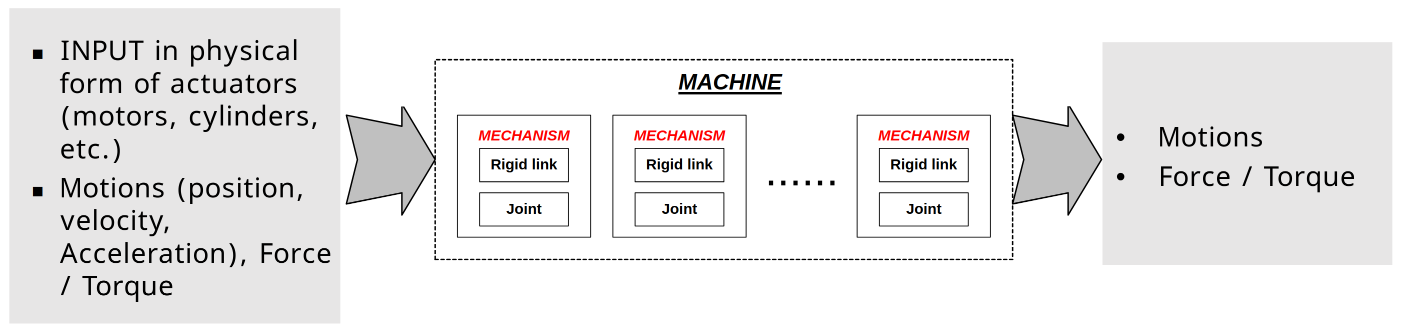
\includegraphics[width=.9\linewidth]{./images/machine-flow-chart.png}
\end{center}
\subsection{Mechanism}
\label{sec:orgaaaaabe}
A mechanism is a component of a machine consisting of two or more solid members (moving elements) connected together by joints.

\begin{center}
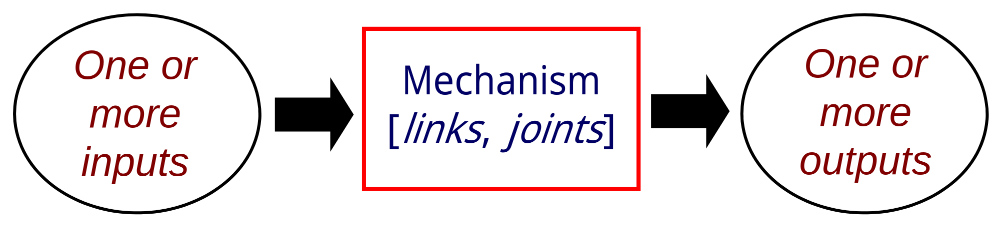
\includegraphics[width=.9\linewidth]{./images/mechanism-flow-chart.png}
\end{center}
\subsection{Kinematics}
\label{sec:org605a1b3}
Study of motions, (position, velocity and acceleration of points and angular position, velocity, and acceleration of rigid bodies) in mechanism without references to forces.
\subsection{Dynamics}
\label{sec:org788f399}
Study of motions in mechanisms with exerted forces and torques.
\subsection{Kinematic analysis}
\label{sec:org1295ef2}
Kinematic analysis is determining position, velocity, and acceleration of points in members of specific mechanisms.

You can use kinematic analysis to evaluate performance.
\subsection{Kinematic synthesis}
\label{sec:org20d47a5}
Kinematic synthesis is determining geometry or dimensions of a mechanism to produce a desired set of position, velocity and acceleration.

You use kinematic synthesis to design something to meet requirements.
\subsection{Link}
\label{sec:orgc968c8f}
Link refers to one of the \textbf{rigid bodies} or members joined together to form a kinematic chain (linkage).

 \newpage
\subsubsection{Degrees of freedom}
\label{sec:org7e594a2}
The number of independent parameters specifies the \textbf{location and configuration} of a rigid link (body).

3 degrees of freedom for a plane:
\begin{center}
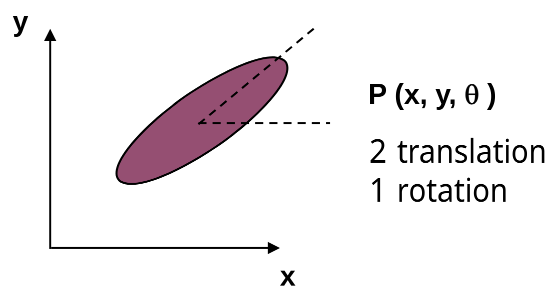
\includegraphics[width=.9\linewidth]{./images/links-plane-degrees-of-freedom-image.png}
\end{center}

6 degrees of freedom for a space:
\begin{center}
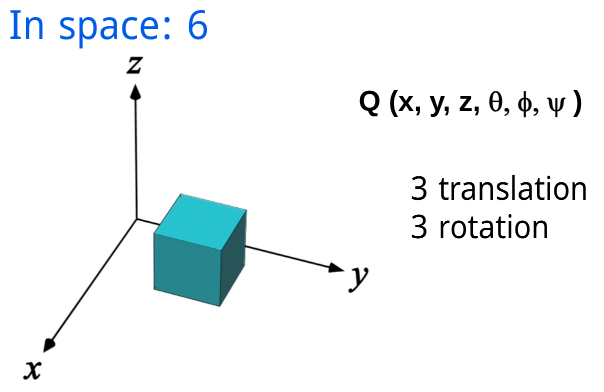
\includegraphics[width=.9\linewidth]{./images/links-space-degrees-of-freedom-image.png}
\end{center}
\subsection{Joint}
\label{sec:orgebd33de}
Joint refers to the connections between links that permit relative movement.
\subsubsection{Classification of joints}
\label{sec:org051fa8a}
\begin{enumerate}
\item Motion (degree of freedom) between connected links:
\begin{itemize}
\item Revolute joints: Revolution, measured by angles, 1 degree of freedom.
\begin{center}
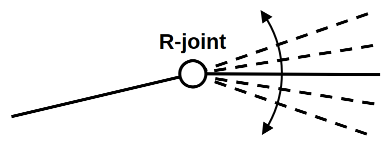
\includegraphics[width=.9\linewidth]{./images/revolute-joint-image.png}
\end{center}

\item Prismatic joints: Linear, measured by distance, 1 degree of freedom.
\begin{center}
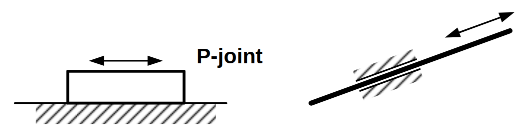
\includegraphics[width=.9\linewidth]{./images/prismatic-joint-image.png}
\end{center}
\end{itemize}

Table:
\begin{center}
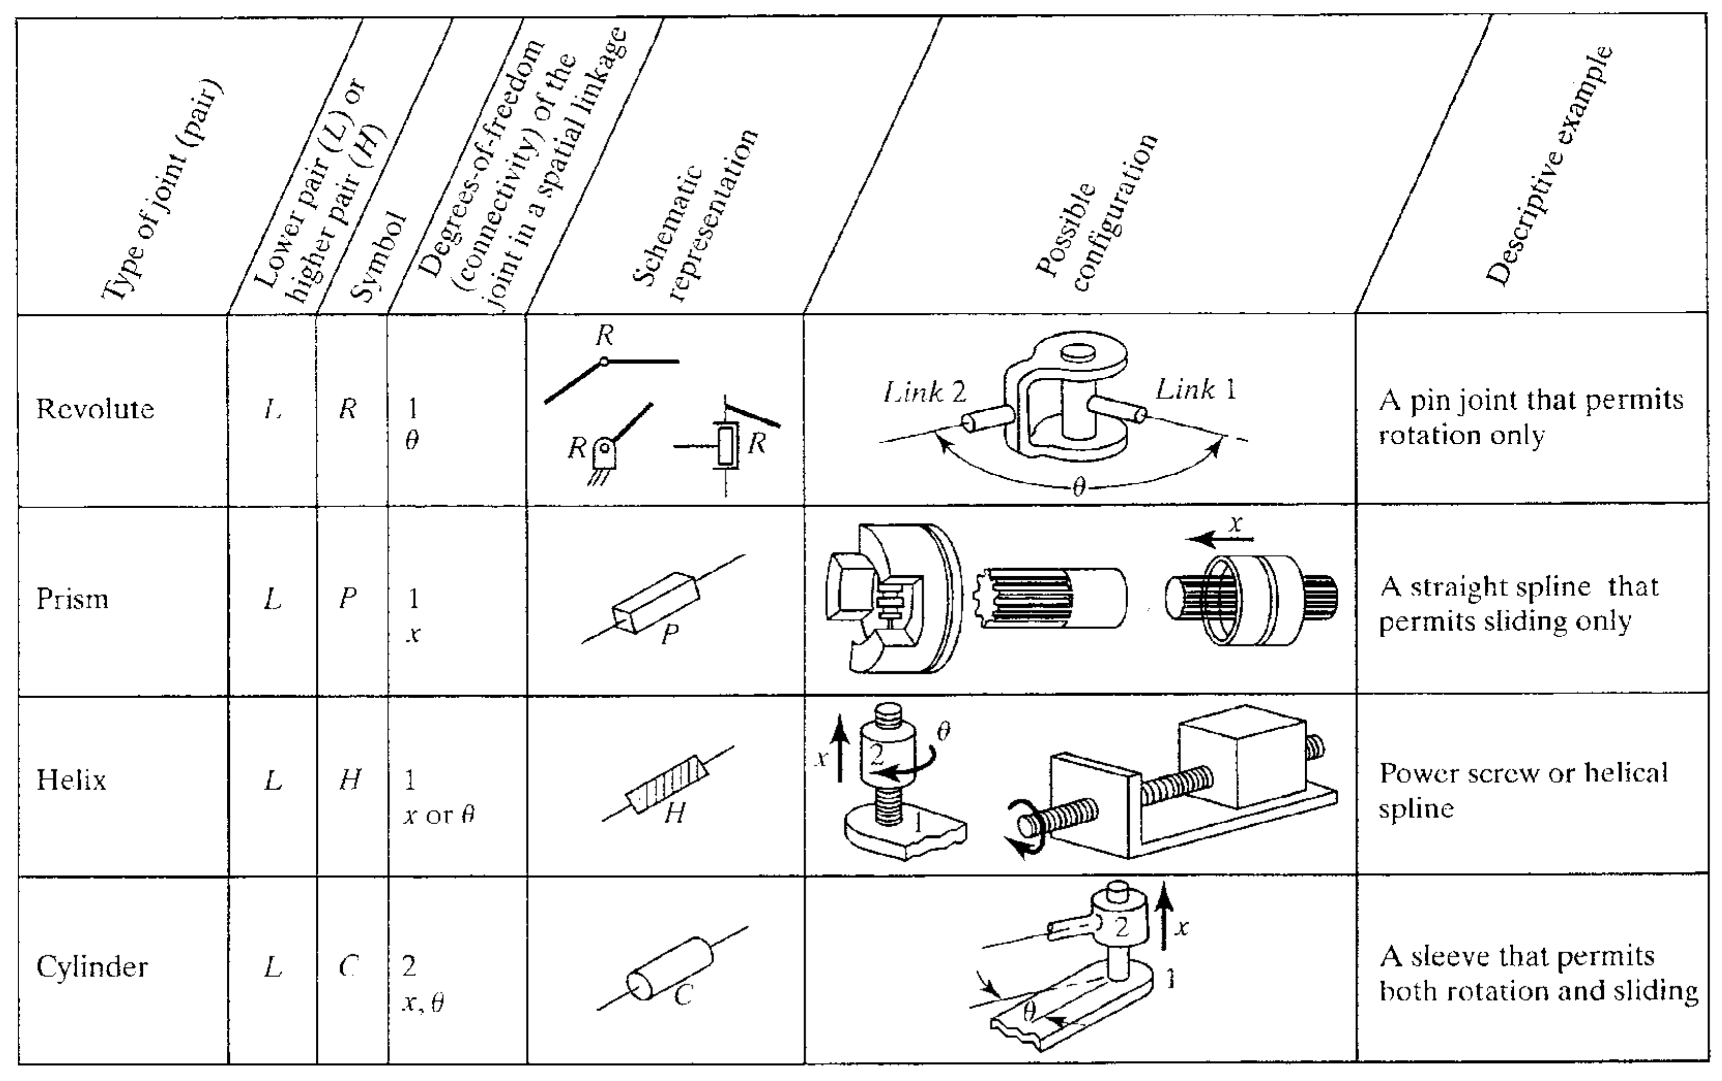
\includegraphics[width=.9\linewidth]{./images/types-of-joints-table.png}
\end{center}
\end{enumerate}

 \newpage

\begin{enumerate}
\item Nature of contact
\begin{itemize}
\item Lower pairs: Surface contact between two links.
\begin{center}
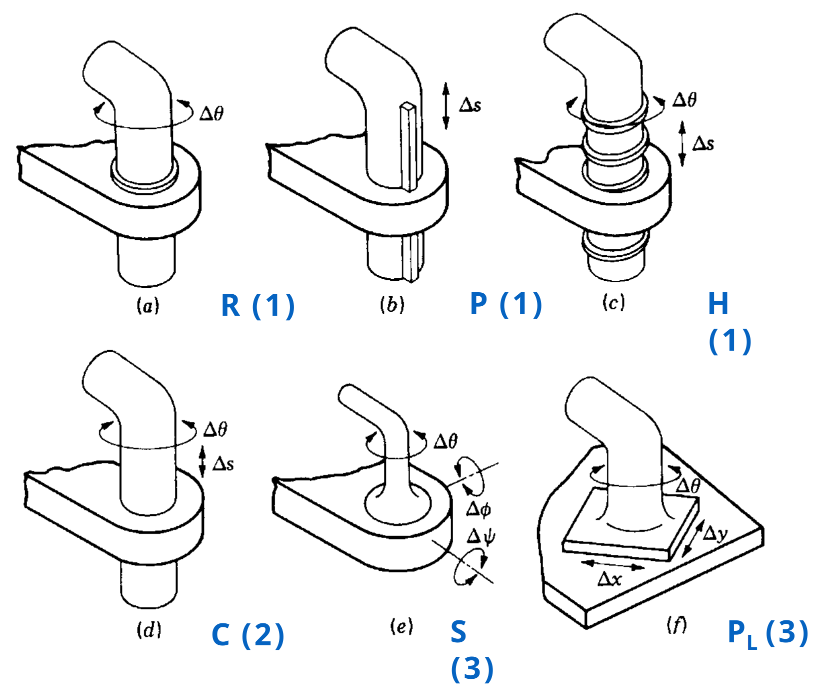
\includegraphics[height=15em]{./images/lower-pair-joints-image.png}
\end{center}

\item Higher pairs: Point or line contact between two links.
\begin{center}
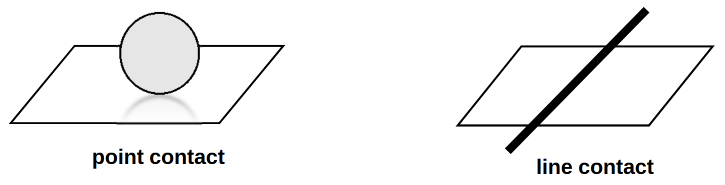
\includegraphics[width=.9\linewidth]{./images/point-and-line-contact-image.png}
\end{center}
\begin{center}
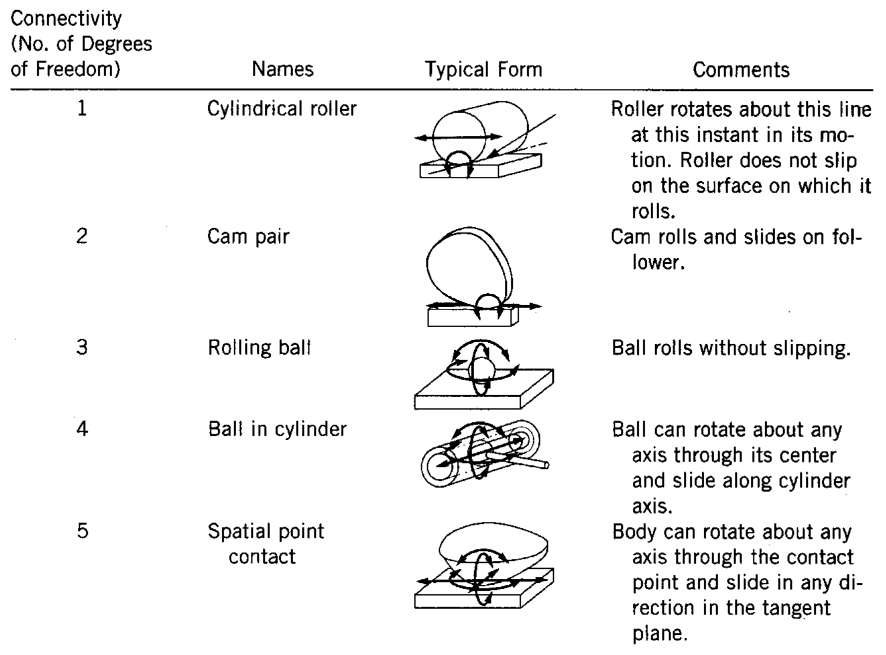
\includegraphics[width=.9\linewidth]{./images/higher-pair-joints-image.png}
\end{center}
\end{itemize}
\end{enumerate}
\subsection{Fixed link / Stationing link}
\label{sec:org498cfe9}
\begin{itemize}
\item A fixed link or stationing link are links between two joints connected to a fixed point.
\item All joints connected to a fixed point are connected to each other through a fixed link.
\end{itemize}
\subsection{Frame}
\label{sec:org184ed0f}
A frame is a fixed or stationing link in a mechanism.
\subsection{Kinematic chains / linkages}
\label{sec:org1bcfbcc}
An assembly of links and joints. It is also known as linkages.
\subsubsection{Open loop linkages}
\label{sec:orga64eb82}
For open loop linkages, the motion of the tip has no constraint. An example is a robot arm.

\begin{center}
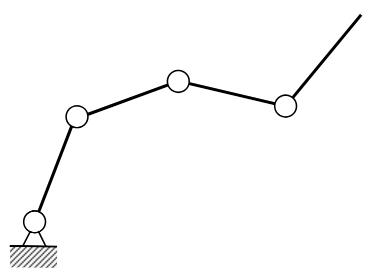
\includegraphics[height=15em]{./images/open-loop-linkage-image.png}
\end{center}

 \newpage
\subsubsection{Closed loop linkages}
\label{sec:orge60d95c}
For closed loop linkages, the motion of the links are constrained by the loop.

\begin{center}
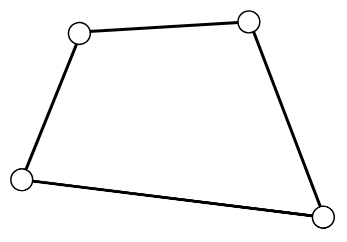
\includegraphics[height=15em]{./images/closed-loop-linkage-image.png}
\end{center}
\subsection{Planar linkages}
\label{sec:org40271aa}
Planar linkages are linkages where the motion of all members are along parallel planes (different layers of planes).

\begin{center}
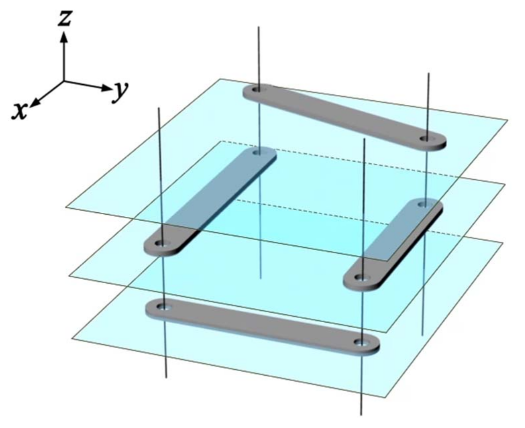
\includegraphics[height=20em]{./images/planar-linkages-image.png}
\end{center}
\subsubsection{Revolute joints}
\label{sec:org609c6dd}
The axes of rotation of revolute joints are normal to the plan.
\subsubsection{Prismatic joint}
\label{sec:org3bff2d6}
The direction of sliding is parallel to the plane.
\subsection{Kinematic diagrams}
\label{sec:org33e45db}
A kinematic diagram is a simplified drawing or sketch of a mechanism showing:
\begin{itemize}
\item Types of links
\item Types of joints
\item Arrangement of links and joints
\item Dimensions of links
\end{itemize}

It is the "skeleton" of the mechanism.
\subsubsection{Types of links}
\label{sec:org8efa73f}
\begin{center}
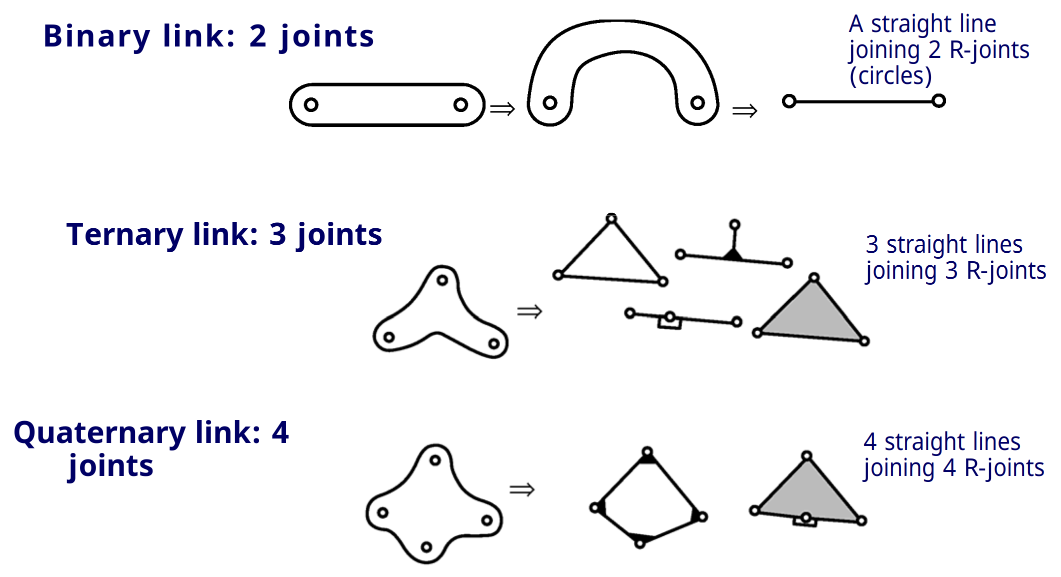
\includegraphics[width=.9\linewidth]{./images/kinematic-diagram-types-of-links.png}
\end{center}
\subsubsection{Types of joints}
\label{sec:org8ccd04b}
\begin{center}
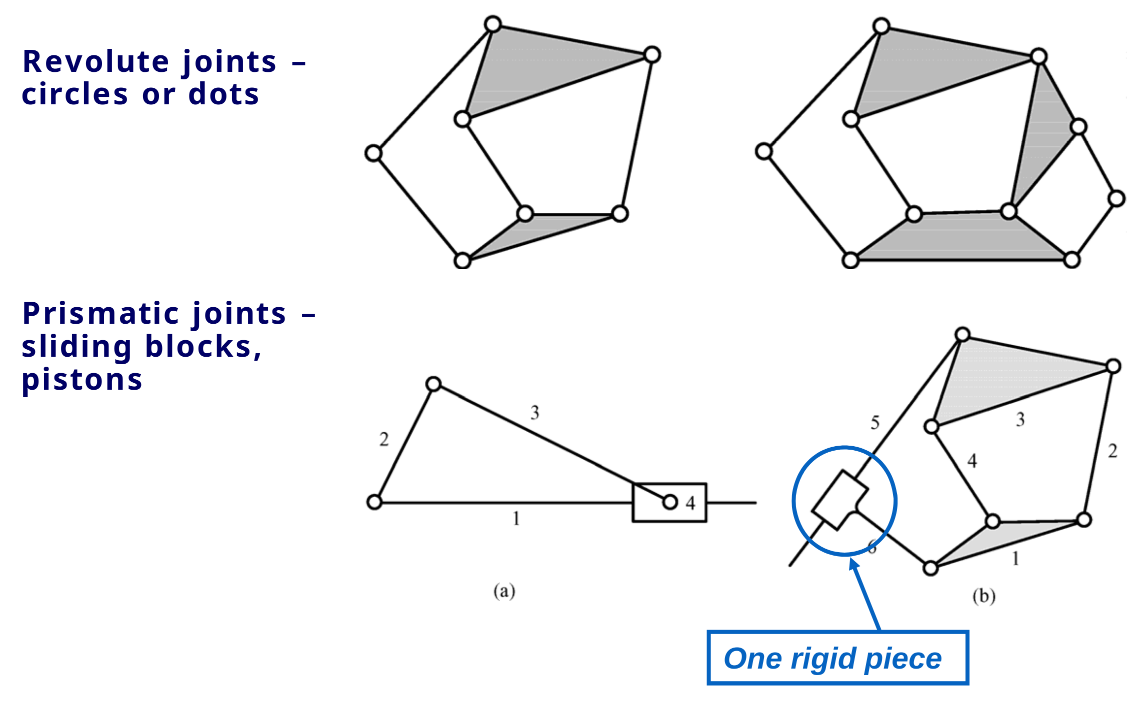
\includegraphics[width=.9\linewidth]{./images/kinematic-diagram-types-of-joints.png}
\end{center}

 \newpage
\subsubsection{Examples}
\label{sec:org7eb8ddc}
\begin{itemize}
\item Vice-grip pliers
\begin{center}
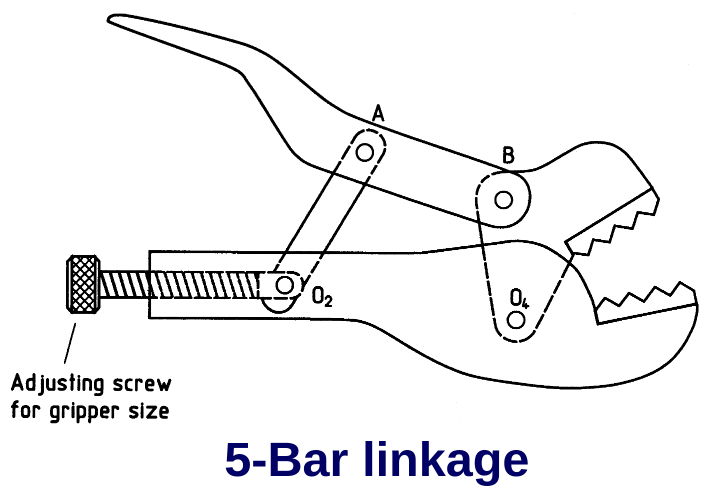
\includegraphics[height=14em]{./images/vice-grip-pliers-kinematic-diagram.png}
\end{center}
\item V-engine
\begin{center}
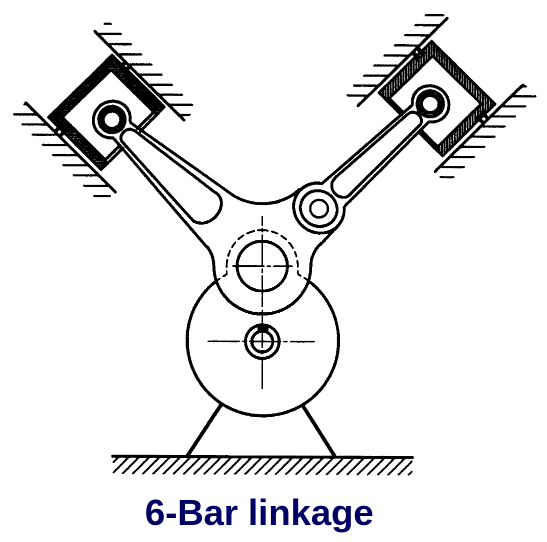
\includegraphics[height=14em]{./images/v-engine-kinematic-diagram.png}
\end{center}
\item Door hinge mechanism
\begin{center}
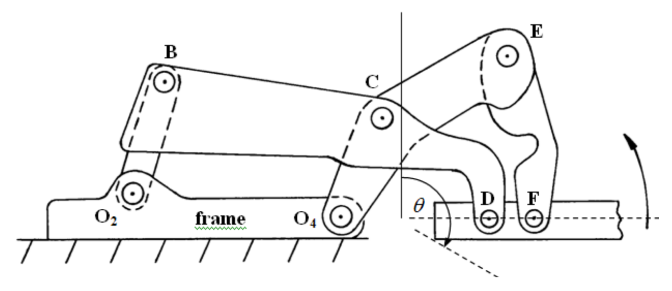
\includegraphics[width=.9\linewidth]{./images/door-hinge-kinematic-diagram.png}
\end{center}
\end{itemize}
\subsection{Multiple joints}
\label{sec:orge5d1d49}
Multiple joints refer to joints that join 3 or more links. These joints need to be counted once more for every link after the second link.
\subsubsection{Actual number of joints}
\label{sec:org380a71a}
The actual number of joints is given by the equation below:
\[\text{Actual number of joints} = \text{Number of links connected to joints } - 1\]
\subsection{Degrees of freedom (DoF) of linkages}
\label{sec:org31ffd56}
\begin{itemize}
\item The degrees of freedom of linkages refers to the number of \textbf{independent} coordinates or parameters needed to specify the position of every link relative to the frame.
\item Motion of connected links are constrained by the number and types of joints in the overall system.
\item The degrees of freedom are always less than the number of joints.
\item The degrees of freedom are \textbf{equal to the number of inputs} (motors, drivers, actuators) to control the mechanism.
\end{itemize}

\begin{center}
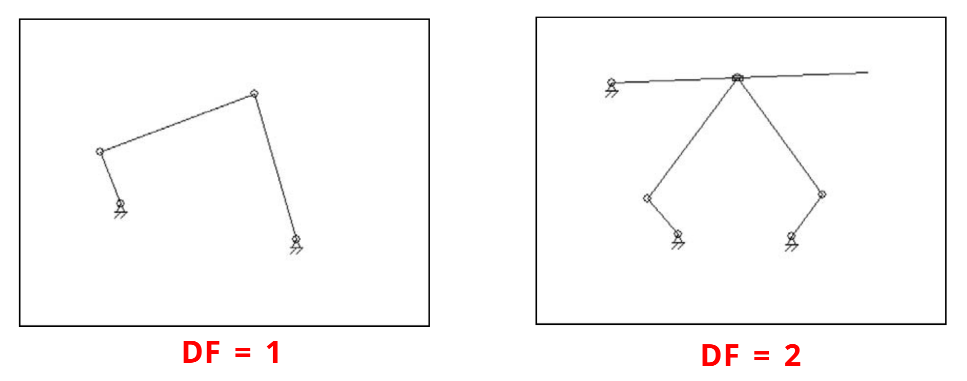
\includegraphics[width=.9\linewidth]{./images/degrees-of-freedom-diagram.png}
\end{center}

 \newpage
\subsubsection{2 DoF example}
\label{sec:org8ad6f51}
Pin-in-slot joints and fork joints have 2 degrees of freedom, 1 for rotation and 1 for rotation.

\begin{center}
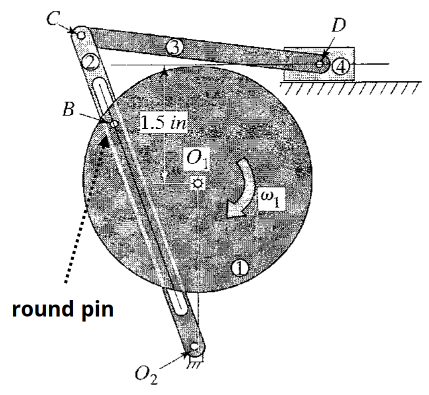
\includegraphics[height=20em]{./images/pin-in-slot-joint.png}
\end{center}

\begin{center}
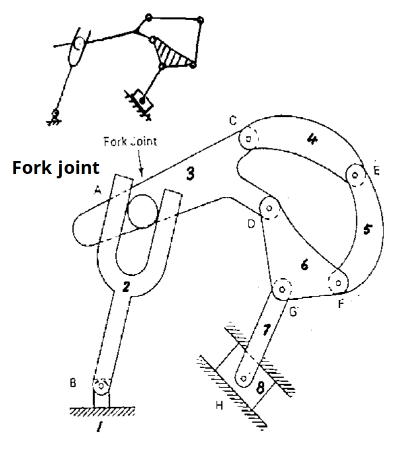
\includegraphics[height=20em]{./images/fork-joint.png}
\end{center}

 \newpage
\subsubsection{Equation}
\label{sec:orgef1dfeb}
\[DF = 3(n_L - 1) - 2n'_J - n''_J\]

Where:
\begin{itemize}
\item \(n_L\) is the number of links
\item \(n'_J\) is the number of 1-DoF joints (revolute and prismatic)
\item \(n''_J\) is the number of 2-DoF joints (round pin in a slot)
\end{itemize}

\begin{center}
\begin{tabular}{l|l}
\(DF > 0\) & Mechanism (movable)\\
\(DF = 0\) & Structure (no moving parts)\\
\(DF < 0\) & Over-constrained structure\\
\end{tabular}
\end{center}
\subsubsection{4-bar linkage}
\label{sec:orgff1aacd}
Four-bar linkage mechanisms are the most frequently used (with either R-joint or P-joint).

\begin{center}
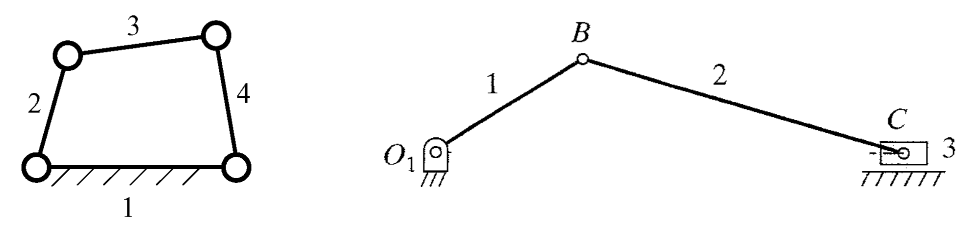
\includegraphics[width=.9\linewidth]{./images/4-bar-linkage-example.png}
\end{center}

\[n_L = 4 \quad n'_J = 4 \quad n''_J = 0\]

\begin{align*}
DF &= 3 (n_L - 1) - 2n'_J - n''_J \\
&= 3 (4 - 1) - 2 \times 4 \\
&= 1
\end{align*}

 \newpage
\subsubsection{Multiple joints}
\label{sec:orgcc42cd2}
\[DF = 3(n_L - 1) - 2n'_J - n''_J\]

\begin{center}
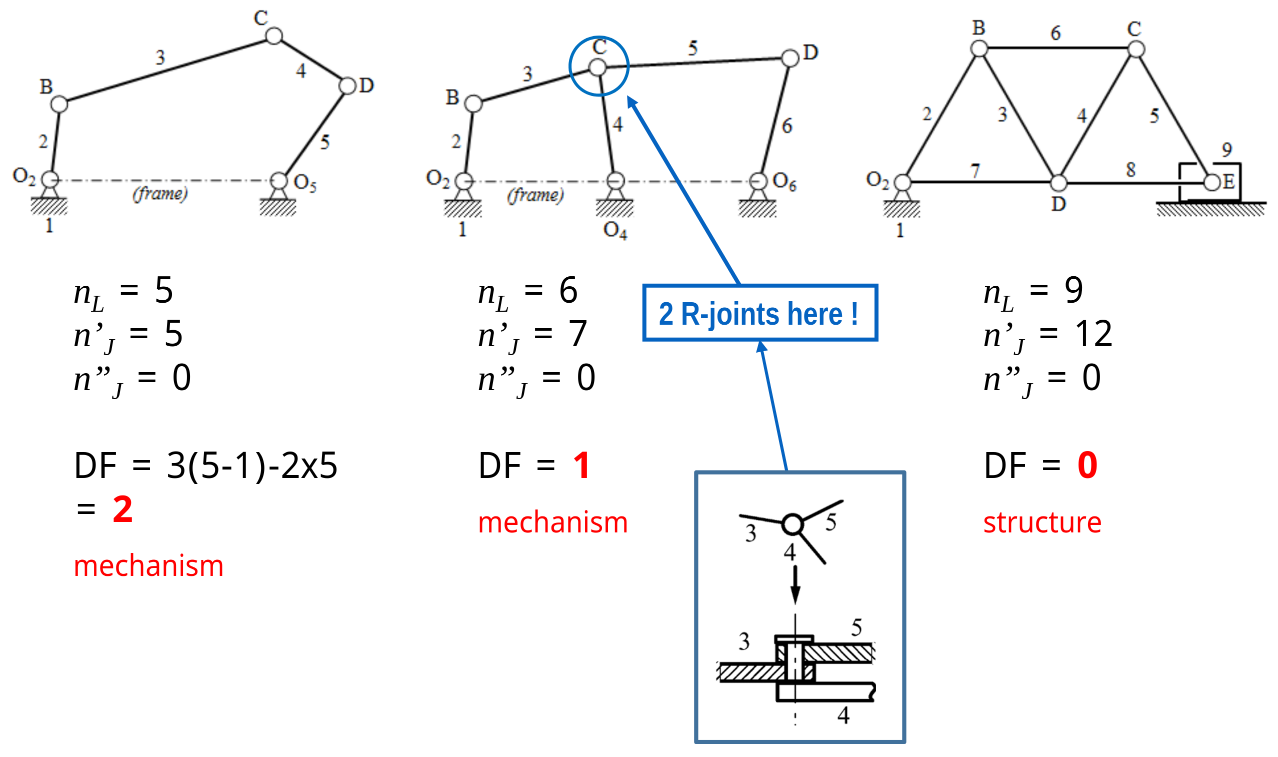
\includegraphics[width=.9\linewidth]{./images/multiple-joints-image.png}
\end{center}
\subsection{Naming convention}
\label{sec:orgef62c06}
Naming conventions are based on input and output relations. A 4-bar linkage has 1 degree of freedom, thus there is one input and one output.

\begin{center}
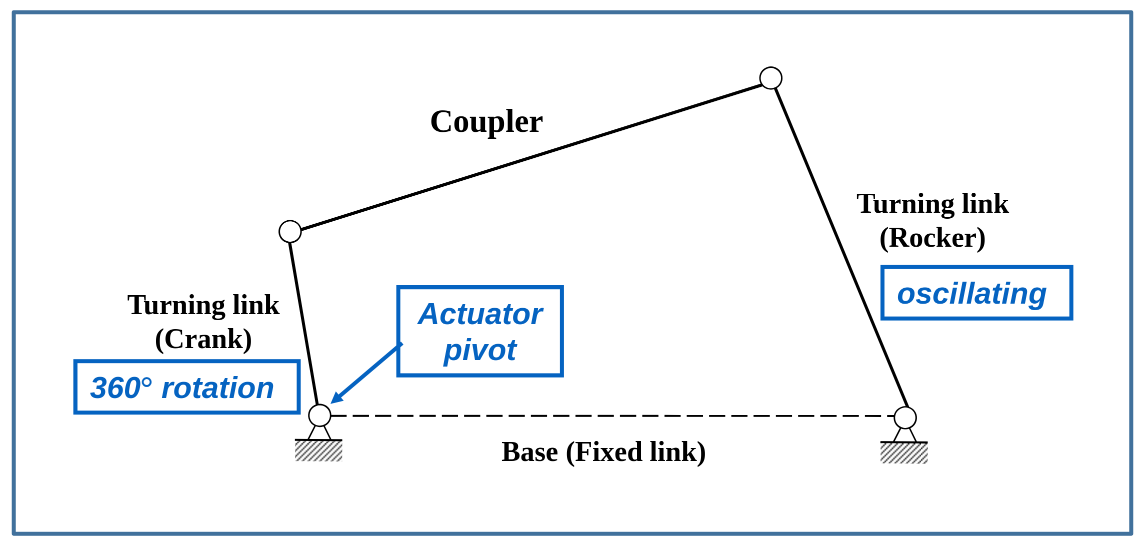
\includegraphics[width=.9\linewidth]{./images/naming-convention.png}
\end{center}

 \newpage
\subsection{Kinematic inversion}
\label{sec:orgd425955}
Choosing different links in a mechanism to be the fixed link or reference frame will result in different motion characteristics.

\begin{center}
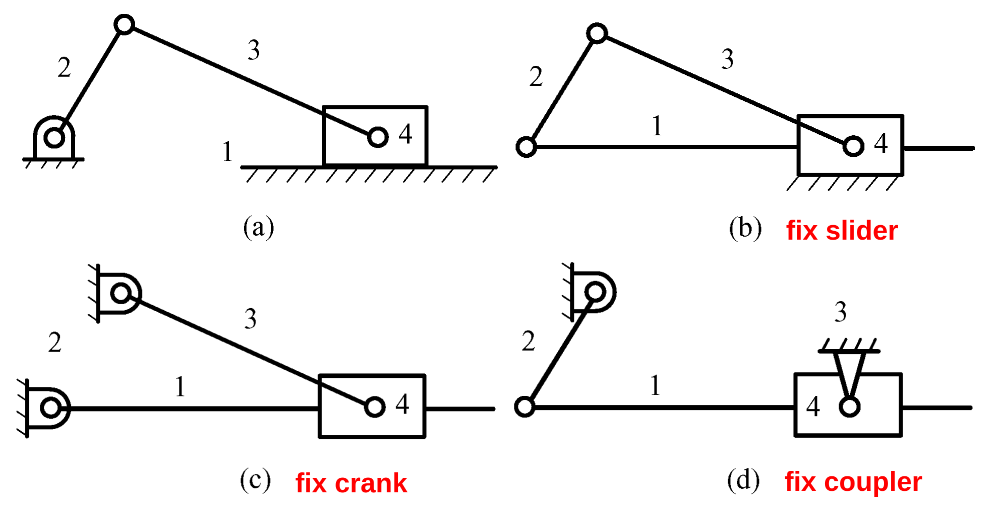
\includegraphics[width=.9\linewidth]{./images/kinematic-inversion-diagram.png}
\end{center}
\subsection{Crank}
\label{sec:orgd7ba758}
A crank is a link that rotates continuously.
\subsection{Condition to form a 4-bar linkage}
\label{sec:org86810f2}
\[L_{max} \le L_{min} + L_a + L_b\]

Where:
\begin{itemize}
\item \(L_{max}\) is the length of the longest link
\item \(L_{min}\) is the length of the shortest link
\item \(L_a, L_b\) are the lengths of the other two links
\end{itemize}

 \newpage
\subsection{Grashof condition}
\label{sec:orgdbc5794}
\begin{center}
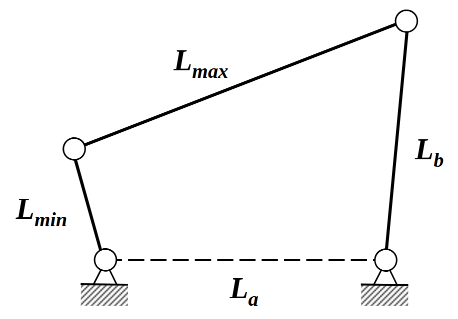
\includegraphics[width=.9\linewidth]{./images/grashof-condition-linkage-image.png}
\end{center}

For a planar 4-bar linkage, if the dimensions of links satisfy the below condition, it is called a \textbf{Grashof} linkage.
\[L_{max} + L_{min} \le L_a + L_b\]

Where:
\begin{itemize}
\item \(L_{max}\) is the length of the longest link
\item \(L_{min}\) is the length of the shortest link
\item \(L_a, L_b\) are the lengths of the other two links  \\
\end{itemize}

Grashof linkages also have at least one link can rotate \(\qty{360}{\degree}\).  \\

If the linkage doesn't satisfy the condition above, the linkage is called a \textbf{non-Grashof} linkage.

 \newpage
\subsubsection{Types of linkages}
\label{sec:orgfe8054d}
\begin{enumerate}
\item Crank-rocker linkage.
\begin{itemize}
\item The shortest link is \textbf{next to the fixed link}.
\item The shortest link rotates \(\qty{360}{\degree}\).
\end{itemize}

\begin{center}
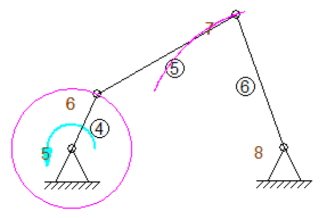
\includegraphics[scale=1]{./images/crank-rocker-linkage-image.png}
\end{center}

\item Drag-link linkage, also known double-crank linkage.
\begin{itemize}
\item The shortest link is the \textbf{fixed link}.
\item Both input and output links rotate \(\qty{360}{\degree}\).
\end{itemize}

\begin{center}
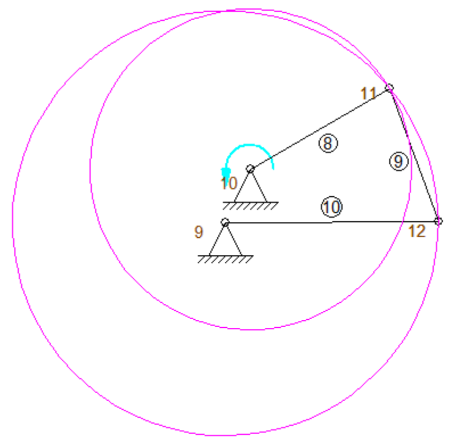
\includegraphics[scale=1]{./images/drag-link-linkage-image.png}
\end{center}

 \newpage

\item Double rocker linkage.
\begin{itemize}
\item Shortest link is opposite the fixed link.
\item The coupler rotates \(\qty{360}{\degree}\).
\end{itemize}

\begin{center}
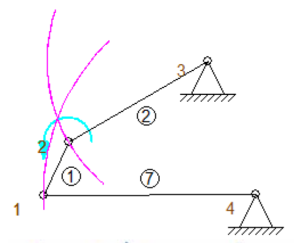
\includegraphics[scale=1]{./images/double-rocker-linkage-image.png}
\end{center}

\item Change-point linkage, also known as crossover-position linkage.
\begin{itemize}
\item All links can be collinear.
\end{itemize}

\begin{center}
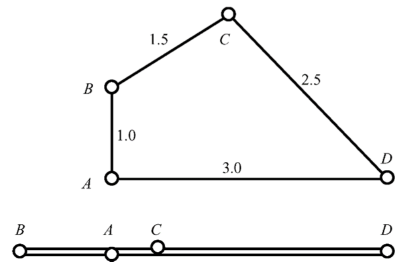
\includegraphics[scale=1]{./images/change-point-linkage-image.png}
\end{center}

\item Triple rocker, which is a non-Grashof linkage.
\begin{itemize}
\item None of the links makes a \(\qty{360}{\degree}\) rotation.
\end{itemize}
\end{enumerate}

 \newpage
\subsection{Transmission angle (\(\phi\))}
\label{sec:orgf1e0886}
\begin{itemize}
\item The transmission angle is the angle between the coupler centreline and the output rocker centreline.

\begin{center}
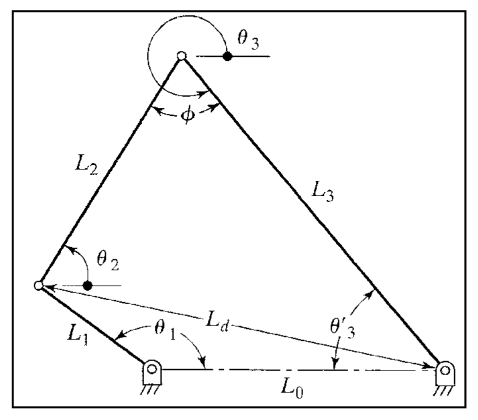
\includegraphics[height=15em]{./images/transmission-angle-image.png}
\end{center}
\item A small transmission angle results in very small output torque on rocker but high bearing force at \(O_3\).
\begin{center}
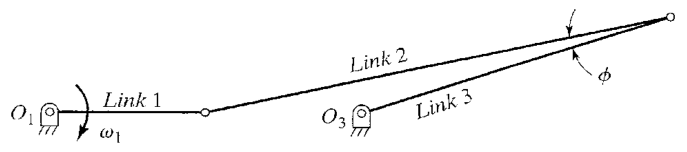
\includegraphics[width=.9\linewidth]{./images/small-transmission-angle-image.png}
\end{center}
\item The usual range of transmission angles is \(\qty{40}{\degree} \le \phi \le \qty{140}{\degree}\).
\item The optimal transmission angle is \(\qty{90}{\degree}\).
\item The minimum and maximum transmission angle occur when the crank aligns with the fixed link.
\begin{center}
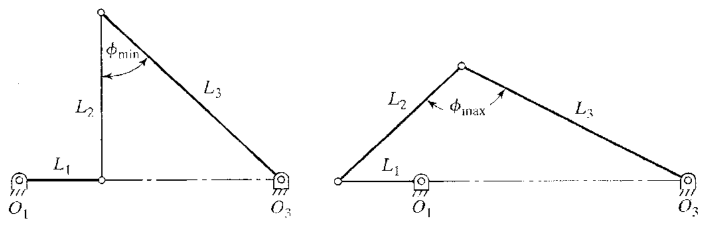
\includegraphics[width=.9\linewidth]{./images/minimum-and-maximum-transmission-angle.png}
\end{center}
\end{itemize}
\subsection{Limiting position}
\label{sec:orgf1a2193}
\begin{itemize}
\item The limiting position occurs when the input link aligns with the coupler.
\item It defines the range of motion of the output link geometrically.
\end{itemize}

\begin{center}
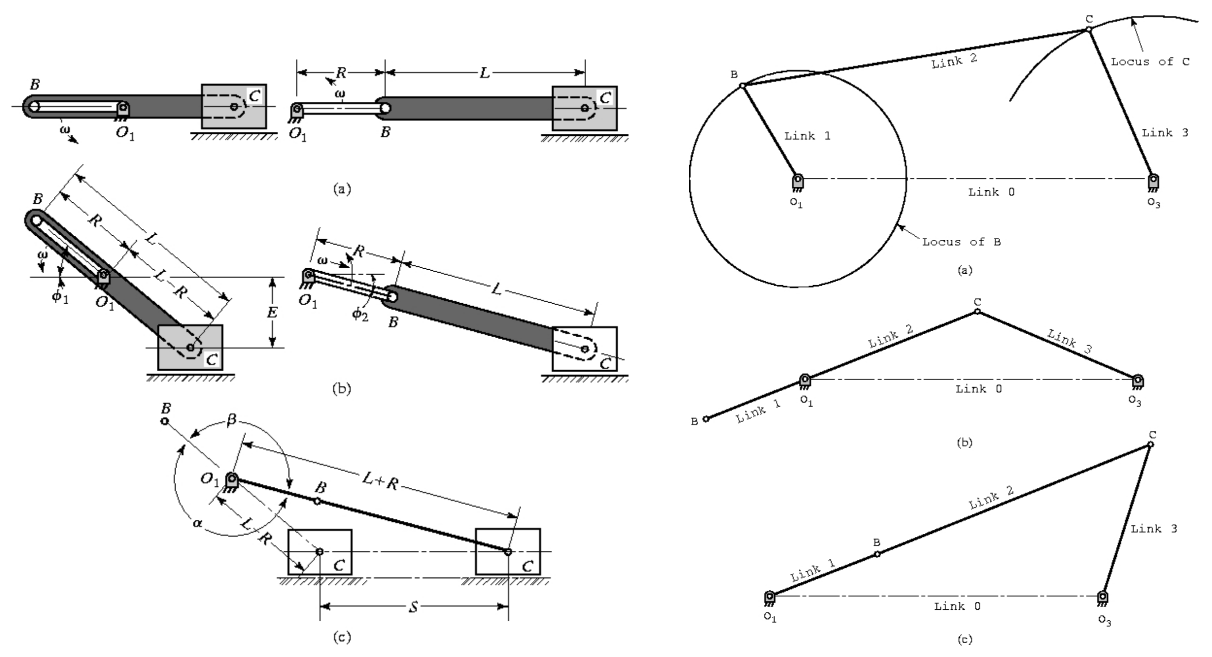
\includegraphics[width=.9\linewidth]{./images/limiting-position-image.png}
\end{center}

 \newpage
\subsection{Two external friction wheels}
\label{sec:orga5f76f1}
\begin{center}
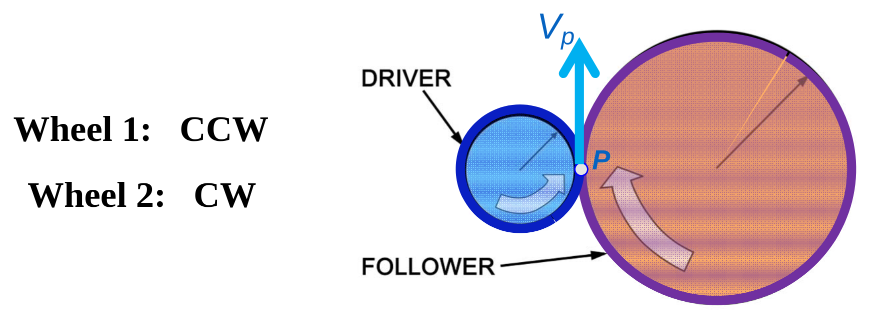
\includegraphics[width=.9\linewidth]{./images/two-external-friction-wheels.png}
\end{center}
\begin{itemize}
\item Wheels are in perfect contact (no slip), instantaneous velocities at contact point, \(P\), should be the same for both wheels.
\item We have:
\[V_p = r_1 \omega_1 = r_2 \omega_2\]
\item Hence:
\[V_r = \frac{\omega_2}{\omega_1} = \frac{r_1}{r_2} \tag{1}\]
\end{itemize}

Where:
\begin{itemize}
\item \(V_p\) is the velocity of the point of contact of both gears
\item \(r_1\) is the radius of one circle
\item \(\omega_1\) is the angular velocity of the circle
\item \(r_2\) is the radius of the other circle
\item \(\omega_2\) is the angular velocity of the other circle
\end{itemize}
\subsection{Two internal friction wheels}
\label{sec:org6c72889}
\begin{center}
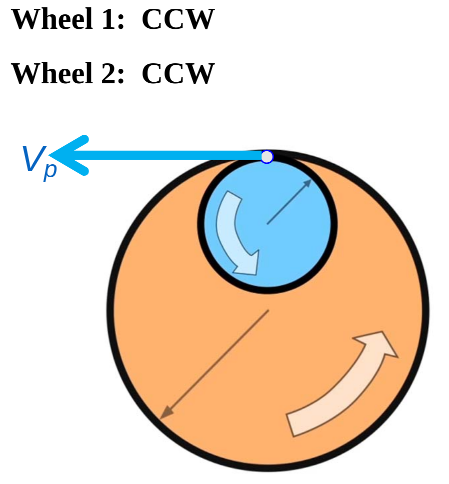
\includegraphics[height=20em]{./images/two-internal-friction-wheels.png}
\end{center}
\begin{itemize}
\item For two internal wheels, equation (\(1\)) above still holds except that two wheels rotate in the same direction.
\end{itemize}

\[V_r = \frac{\omega_2}{\omega_1} = \frac{r_1}{r_2} \tag{1}\]

Where:
\begin{itemize}
\item \(V_p\) is the velocity of the point of contact of both gears
\item \(r_1\) is the radius of one circle
\item \(\omega_1\) is the angular velocity of the circle
\item \(r_2\) is the radius of the other circle
\item \(\omega_2\) is the angular velocity of the other circle
\end{itemize}
\subsection{Gears}
\label{sec:org87d771b}
Gears are used to transmit power and displacement between shafts.
\subsection{Laws of gearing}
\label{sec:org026d9d0}
\begin{center}
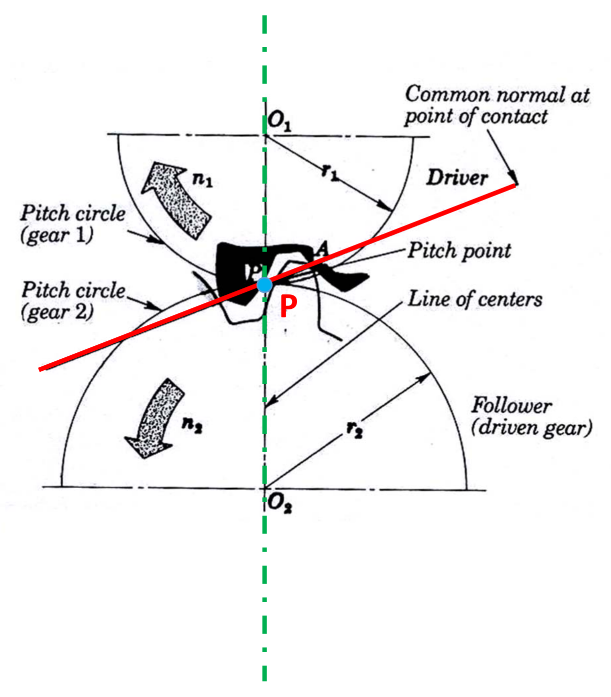
\includegraphics[width=.9\linewidth]{./images/common-normal-at-point-of-contact.png}
\end{center}
\begin{itemize}
\item To maintain constant angular velocity ratio, the shape (profile) of teeth of a gear requires that \textbf{a common normal} at the point of contact between two teeth always passes through a fixed point on the line of centres of the gears.
\item This point is called the \textbf{pitch} point.
\item When the fundamental law is satisfied, gears in mesh are said to produce \textbf{conjugate action}.
\item The involute tooth profile provides this constant velocity ratio.
\end{itemize}
\subsection{Spur gear terminology}
\label{sec:org149aed7}
\begin{center}
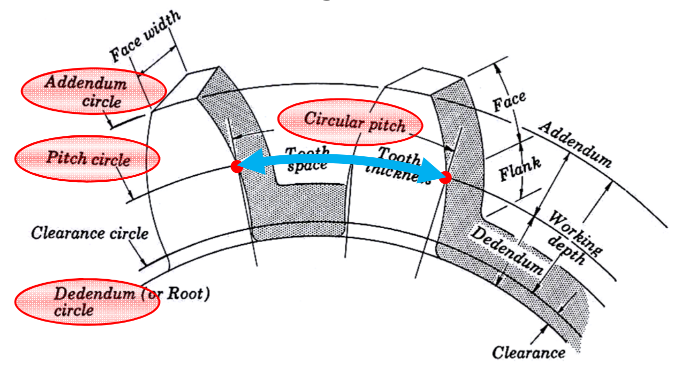
\includegraphics[width=.9\linewidth]{./images/spur-gear-terminology.png}
\end{center}
\subsubsection{Pitch circle}
\label{sec:org7eb84b1}
The pitch circle is the circle on a gear that corresponds to the contact point of a friction wheel.
\subsubsection{Addendum circle}
\label{sec:orgdf8b1ea}
The addendum circle is the circle drawn through the top of the gear tooth, and its centre is at the gear centre.
\subsubsection{Dedendum circle}
\label{sec:orgf6d5bbe}
The dedendum circle is the circle drawn through the bottom of the gear tooth, and its centre is at the gear centre.

 \newpage
\subsubsection{Circular pitch}
\label{sec:org8521448}
The circular pitch is the arc distance along the pitch circle from a point on one tooth to the corresponding point on the adjacent tooth of the gear.

\[p_c = \frac{\pi d_p}{N} = \pi m\]

Where:
\begin{itemize}
\item \(p_c\) is the circular pitch
\item \(d_p\) is the pitch diameter of the gear, which is the diameter of the pitch circle on the gear
\item \(N\) is the number of teeth on the gear
\item \(m\) is the module of the gear
\end{itemize}
\subsection{Module (\(m\))}
\label{sec:org127d320}
Module \(m\) in SI units is used to express the gear tooth size rather than the diametral pitch \(P\) used in US units.

\[m = \frac{d_p}{N}\]

Where:
\begin{itemize}
\item \(m\) is the module of the gear, or the gear tooth size in millimetres (\(\unit{mm}\))
\item \(d_p\) is the pitch diameter of the gear, which is the diameter of the pitch circle on the gear
\item \(N\) is the number of teeth on the gear
\end{itemize}
\subsubsection{Converting to diametral pitch (\(P\))}
\label{sec:org7416cec}
\[\frac{m}{25.4} = \frac{1}{P}\]

Where:
\begin{itemize}
\item \(m\) is the module of the gear, or the gear tooth size in millimetres (\(\unit{mm}\))
\item \(P\) is the diametral pitch of the gear
\end{itemize}
\subsection{Radius in terms of module (\(r\))}
\label{sec:org994cf89}
\[r = \frac{mN}{2}\]

Where:
\begin{itemize}
\item \(r\) is the radius of the pitch circle of the gear
\item \(m\) is the module of the gear
\item \(N\) is the number of teeth on the gear
\end{itemize}
\subsection{Tooth thickness in terms of module (\(t\))}
\label{sec:orgf296a0a}
\[t = \frac{\pi}{2} m\]

Where:
\begin{itemize}
\item \(t\) is the tooth thickness
\item \(m\) is the module
\end{itemize}

 \newpage
\subsection{Base circle}
\label{sec:orged6ddc3}
\begin{center}
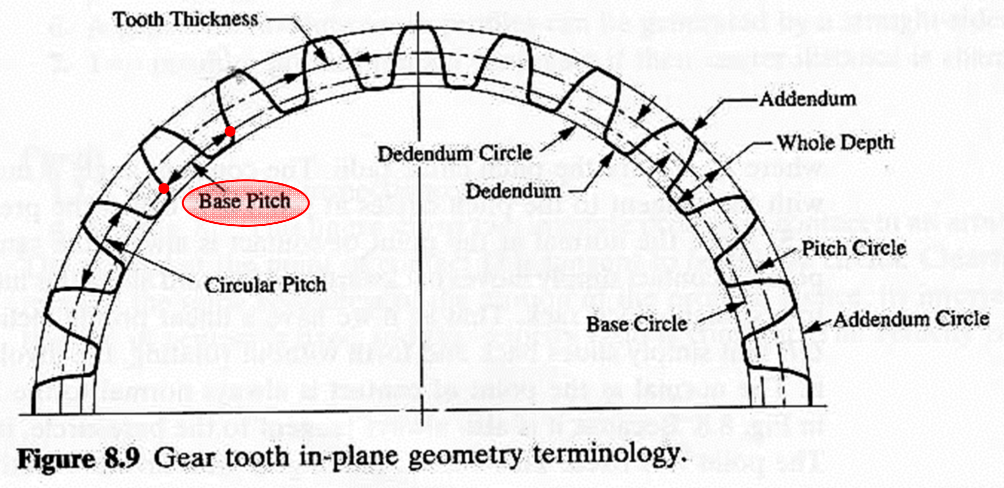
\includegraphics[width=.9\linewidth]{./images/base-circle-diagram.png}
\end{center}
\subsubsection{Addendum (\(a\))}
\label{sec:orgd6ab950}
The addendum is the length of the top half of the gear tooth. It should be equal to the dedendum. It is equal to the module of the gear, i.e.

\[a = m\]

Where:
\begin{itemize}
\item \(a\) is the addendum of the gear
\item \(m\) is the module of the gear
\end{itemize}
\subsubsection{Dedendum}
\label{sec:org4f0ae17}
The dedendum is the length of the bottom half of the gear tooth. It should be equal to the addendum.

 \newpage
\subsection{Velocity ratio}
\label{sec:org55e5179}
\begin{itemize}
\item The velocity ratio is equal to the angular speed (\(\omega\)) of the follower or driven gear (\(\omega_2\)) divided by the angular speed of the driving gear (\(\omega_1\)), i.e.
\[r_v = \frac{\omega_2}{\omega_1}\]
Where:
\begin{itemize}
\item \(r_v\) is the velocity ratio
\item \(\omega_2\) is the angular velocity of the follower or driven gear
\item \(\omega_1\) is the angular velocity of the driving gear
\end{itemize}

\item It can also be expressed in terms of the ratio of rounds per minutes (RPM), the pitch radii, and the number of gear teeth:
\[r_v = \frac{\omega_2}{\omega_1} = \frac{RPM_2}{RPM_1} = \frac{r_1}{r_2} = \frac{N_1}{N_2}\]
\end{itemize}
\subsection{Centre distance}
\label{sec:orge921997}
\begin{center}
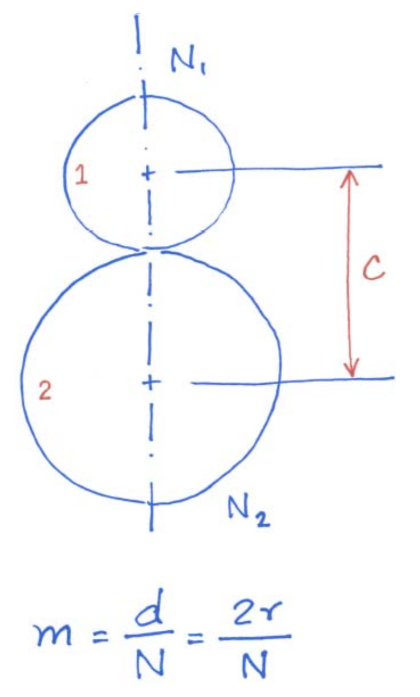
\includegraphics[height=15em]{./images/centre-distance-image.png}
\end{center}
\begin{itemize}
\item The centre distance is the distance \(c\) shown in the image above.
\item This distance represents the spacing between the centres of the shafts upon which the gears are mounted.
\end{itemize}
\subsubsection{In terms of pitch diameter (\(d_p\))}
\label{sec:orgb567d69}
\[c = \frac{d_{p1} + d_{p2}}{2}\]

Where:
\begin{itemize}
\item \(c\) is the centre distance
\item \(d_{p1}\) is the pitch diameter of the first gear
\item \(d_{p2}\) is the pitch diameter of the second gear
\end{itemize}
\subsubsection{In terms of module in SI units (\(m\))}
\label{sec:orgba4558c}
\[c = \frac{m (N_1 + N_2)}{2}\]

Where:
\begin{itemize}
\item \(c\) is the centre distance
\item \(m\) is the module of the gears
\item \(N_1\) is the number of teeth on the first gear
\item \(N_2\) is the number of teeth on the second gear
\end{itemize}
\subsubsection{In terms of diametral pitch in English units (\(P_d\))}
\label{sec:orgb4c7cb0}
\[c = \frac{N_1 + N_2}{2 P_d}\]

Where:
\begin{itemize}
\item \(N_1\) is the number of teeth on the first gear
\item \(N_2\) is the number of teeth on the second gear
\end{itemize}

 \newpage
\subsection{Line of action}
\label{sec:org8fec96f}
\begin{center}
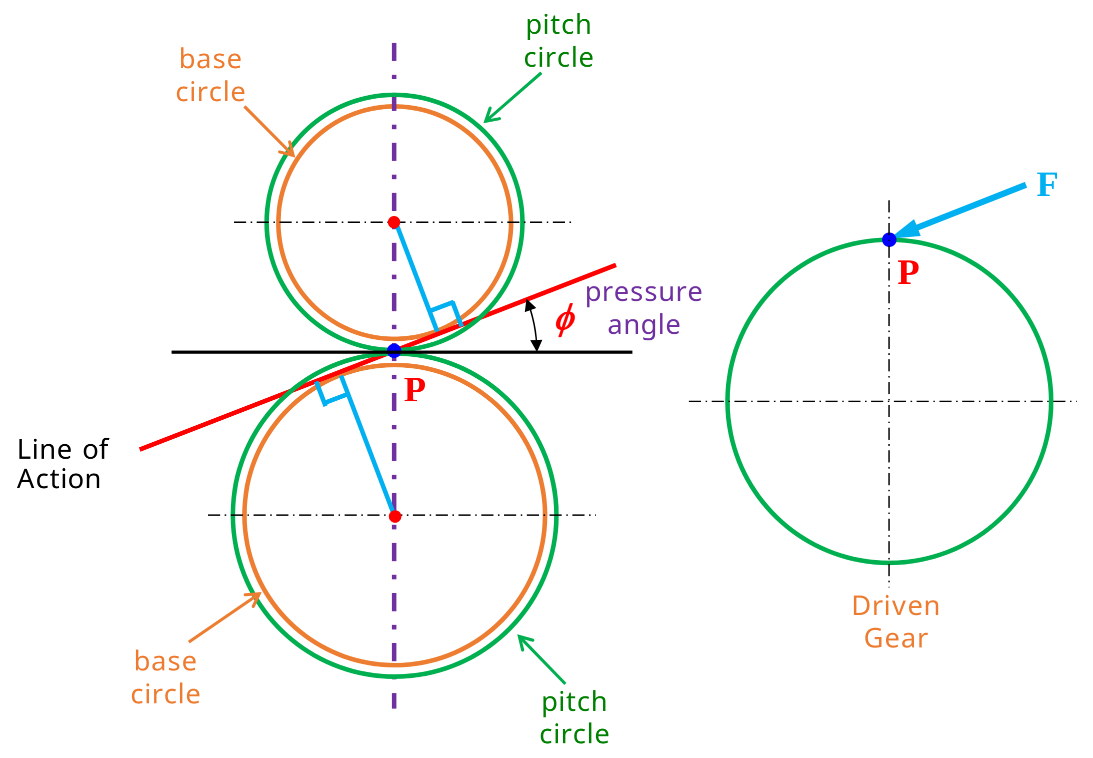
\includegraphics[width=.9\linewidth]{./images/gear-contact-geometry-diagram.png}
\end{center}
\begin{itemize}
\item The red line in the image above is called the line of action because the contact points of two gears in mesh must lie along it.
\item The force that one gear tooth exerts on the tooth of the meshing gear acts along the common normal, which is also the red line in the image above.
\item Therefore, another name commonly given to the line of action is the pressure line.
\end{itemize}
\subsection{Pressure angle (\(\phi\))}
\label{sec:orgedaae5e}
\begin{center}
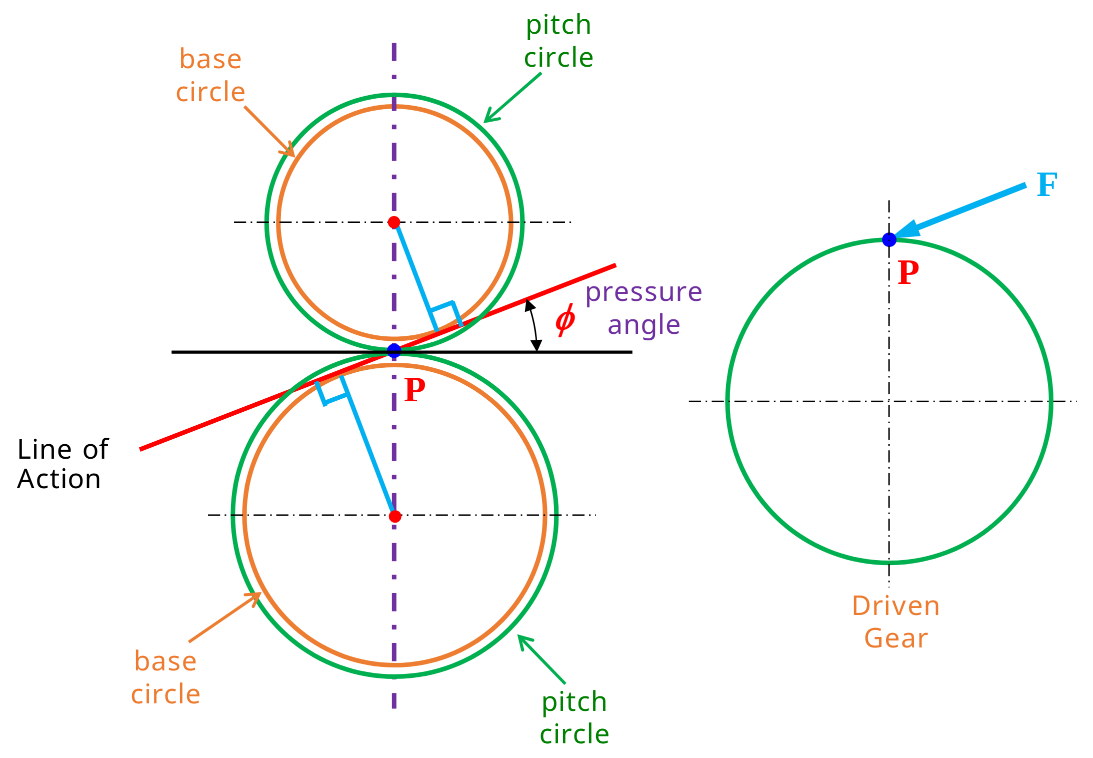
\includegraphics[width=.9\linewidth]{./images/gear-contact-geometry-diagram.png}
\end{center}
\begin{itemize}
\item The angle \(\phi\) between the line of action and the common tangent to the pitch circles of both gears is called the pressure angle.
\item Most gears have a \(\qty{20}{\degree}\) or \(\qty{25}{\degree}\) pressure angle.
\item Gears are designated by their pressure angles, but one has to be careful.
\item Changes in the centre distance will result in changes in the pressure angle.
\end{itemize}
\subsubsection{Relationship between base-circle radius and pitch-circle radius}
\label{sec:org3dae253}
\begin{center}
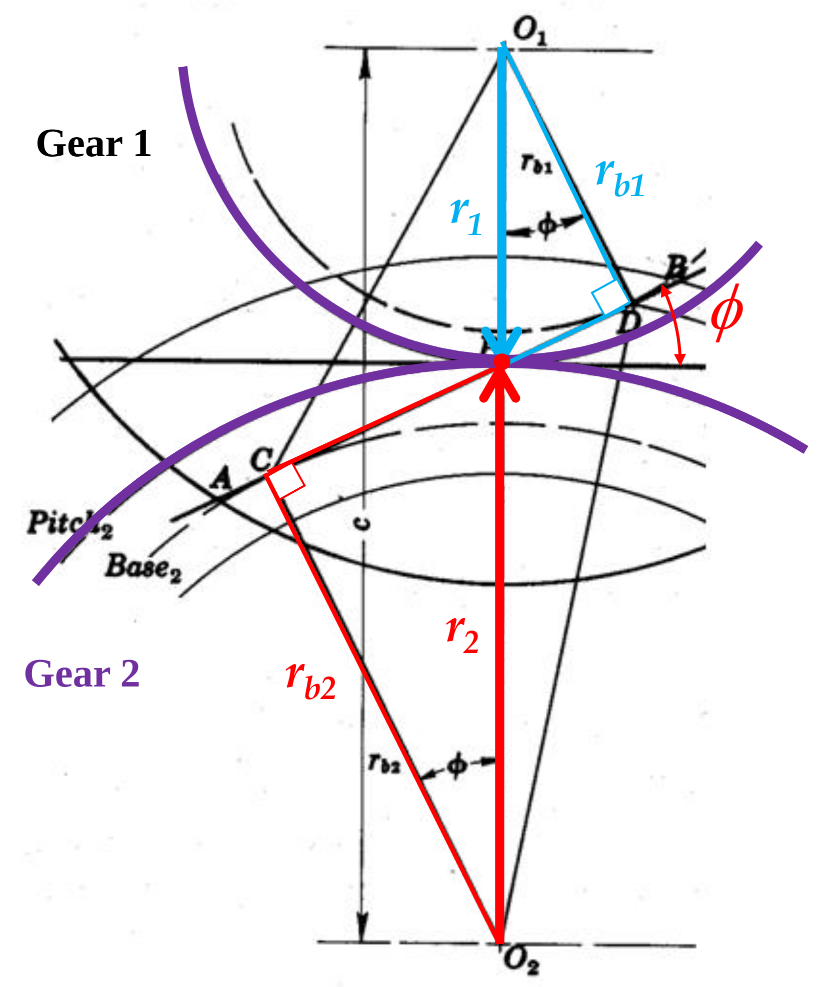
\includegraphics[height=25em]{./images/relationship-between-base-circle-radius-and-pitch-circle-radius-diagram.png}
\end{center}

One of the properties of an involute tooth profile is that the normal to the involute at any point of the curve is tangent to the base circle.

\[r_{b1} = r_1 \cos \phi\]
\[r_{b2} = r_2 \cos \phi\]

Where:
\begin{itemize}
\item \(r_{b1}\) is the radius of the base circle for the first gear
\item \(r_1\) is the radius of pitch circle for the first gear
\item \(\phi\) is the pressure angle between the two gears
\item \(r_{b2}\) is the radius of the base circle for the second gear
\item \(r_2\) is the radius of pitch circle for the second gear
\end{itemize}
\subsection{Meshing conditions}
\label{sec:orgf31fe7f}
For two gears to mesh, the following conditions are required:
\begin{itemize}
\item Pressure angle must be the same.
\item Modules \(m\) (or diametral pitches \(P_d\)) must be the same.
\item Gears must have the same addendum and dedendum.
\item Tooth thickness must be equal to one-half the circular pitch.
\item Gears must have the same circular pitch.
\end{itemize}
\subsection{Pinion}
\label{sec:org97218a8}
A pinion is the \textbf{smaller} gear in a pair of meshing gears, and is the driver gear.
\subsection{Base pitch}
\label{sec:org0a06b03}
\begin{center}
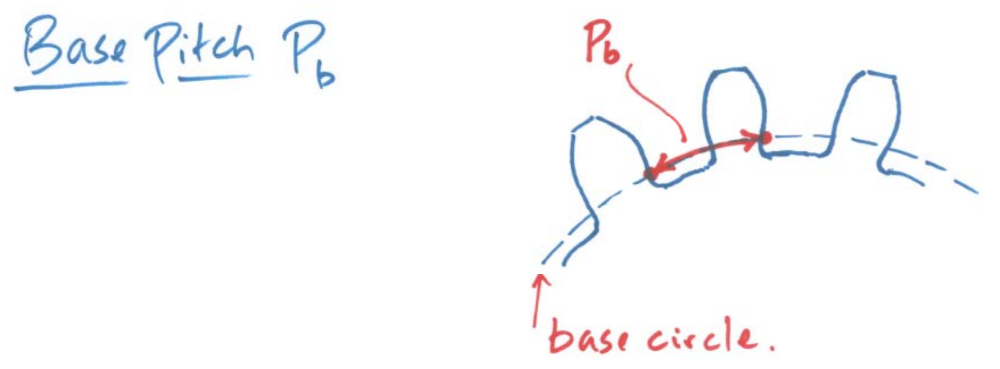
\includegraphics[width=.9\linewidth]{./images/base-pitch-diagram.png}
\end{center}

The base pitch is the arc distance along the \textbf{base circle} from a point on one tooth to the corresponding point on the adjacent tooth of the gear.
\subsubsection{In terms of module in SI units (\(m\))}
\label{sec:org9df7c7c}
\[p_b = m \pi \cos \phi\]

Where:
\begin{itemize}
\item \(p_b\) is the base pitch of the gears
\item \(m\) is the module of the gears
\item \(\phi\) is the pressure angle between the two gears
\end{itemize}

 \newpage
\subsubsection{In terms of diametral pitch in English units (\(P\))}
\label{sec:orgd3d3d2e}
\[p_b = \frac{\pi}{P} \cos \phi\]

Where:
\begin{itemize}
\item \(p_b\) is the base pitch of the gears
\item \(P\) is the diametral pitch of the gears
\item \(\phi\) is the pressure angle between the two gears
\end{itemize}
\subsection{Contact ratio (\(C.R.\))}
\label{sec:org706b17c}

\subsubsection{Diagram}
\label{sec:orgf115952}
\begin{center}
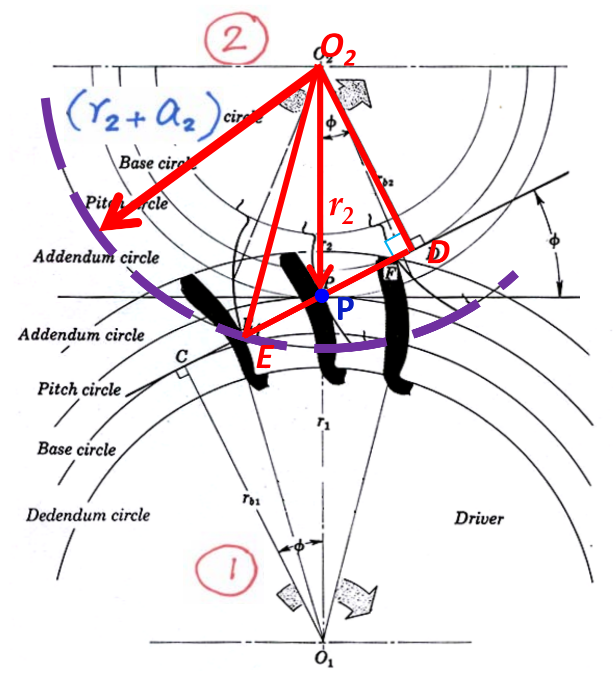
\includegraphics[width=.9\linewidth]{./images/contact-ratio-diagram.png}
\end{center}
\subsubsection{Description}
\label{sec:org4ce5d36}
\begin{itemize}
\item The contact ratio is an indicator of the \textbf{average number of pairs of teeth} in contact.
\item The contact ratio being equal to 1 (\(C.R. = 1\)) means that there is only one pair of teeth in contact.
\end{itemize}
\[C.R. = \frac{\sqrt{(r_2 + a_2)^2 - r_2^2 \cos^2 \phi} - r_2 \sin \phi}{p_b} + \frac{\sqrt{(r_1 + a_1)^2 - r_1^2 \cos^2 \phi} - r_1 \sin \phi}{p_b}\]
Where:
\begin{itemize}
\item \(C.R.\) is the contact ratio
\item \(r_2\) is the radius of pitch circle for the second gear
\item \(a_2\) is the addendum for the second gear
\item \(\phi\) is the pressure angle between the two gears
\item \(p_b\) is the base pitch of the gears
\end{itemize}
\subsection{Interference}
\label{sec:org2eb7be1}
\begin{center}
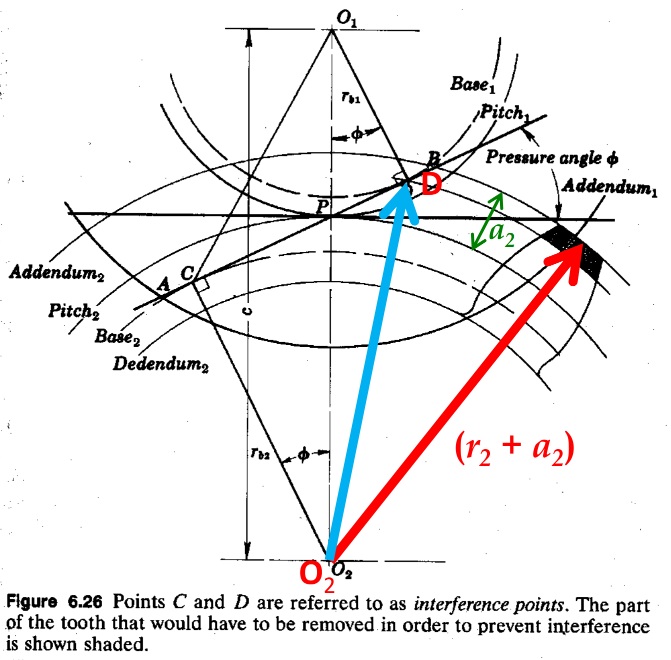
\includegraphics[width=.9\linewidth]{./images/interference-diagram.png}
\end{center}
\begin{itemize}
\item Involute gear teeth have involute profiles between the \textbf{base circle} and the \textbf{addendum circle}.
\item Below the base circle, there is no involute profile.
\item If contact between the two gears occurs below the base circle of one of the gears, interference is said to occur.
\end{itemize}
\subsubsection{Avoiding interference}
\label{sec:org6c74963}
\begin{center}
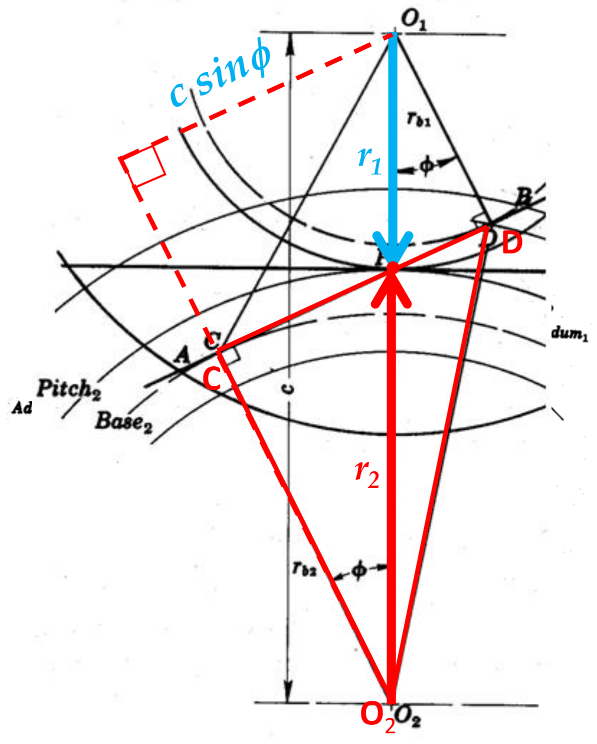
\includegraphics[height=18em]{./images/avoiding-interference-diagram.png}
\end{center}

To avoid interference, the following conditions must be met:

\[r_1 + a_1 \le \sqrt{r_1^2 \cos^2 \phi + c^2 \sin^2 \phi}\]
\[r_2 + a_2 \le \sqrt{r_2^2 \cos^2 \phi + c^2 \sin^2 \phi}\]

Where:
\begin{itemize}
\item \(r_1\) is the radius of the pitch circle of the first gear
\item \(a_1\) is the addendum of the first gear
\item \(\phi\) is the pressure angle between the two gears
\item \(r_2\) is the radius of the pitch circle of the second gear
\item \(a_2\) is the addendum of the second gear
\end{itemize}

For gear 2, the expression can be simplified to:
\[r_2 + a_2 \le O_2 D\]

Where:
\begin{itemize}
\item \(r_2\) is the radius of the pitch circle of the second gear
\item \(a_2\) is the addendum of the second gear
\item \(O_2 D\) is the length defined in the diagram above
\end{itemize}
\subsubsection{Interference of rack and pinion}
\label{sec:orga4b3669}
\begin{center}
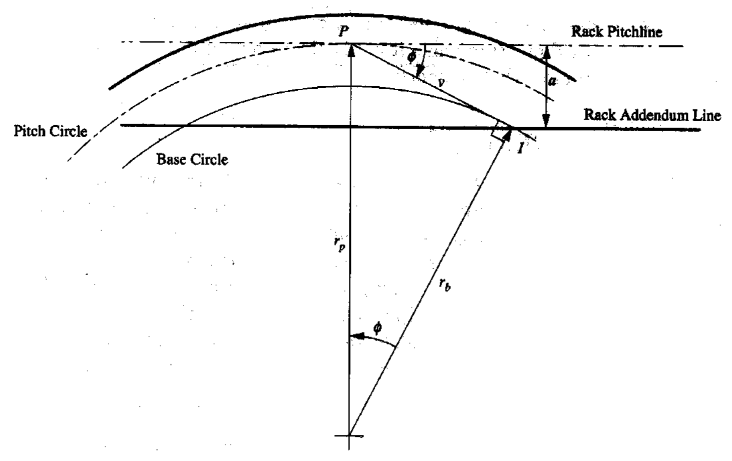
\includegraphics[width=.9\linewidth]{./images/interference-of-rack-and-pinion-diagram.png}
\end{center}
\begin{itemize}
\item The worst possible case for interference.
\item If interference does not occur under this condition, it will never occur to the pinion when it meshes with a gear with the same or more teeth.
\item To avoid interference between a pinion and a rack, the number of teeth on the pinion, \(N\), must satisfy the following condition.
\end{itemize}

\[N \ge \frac{2k}{\sin^2 \phi}\]

Where:
\begin{itemize}
\item \(N\) is the number of teeth on the pinion
\item \(k\) is the addendum constant (in \(\unit{km}\))
\item \(\phi\) is the pressure angle between the rack and the pinion
\end{itemize}
\subsubsection{Minimum number of teeth to avoid interference}
\label{sec:org572d71b}
\begin{center}
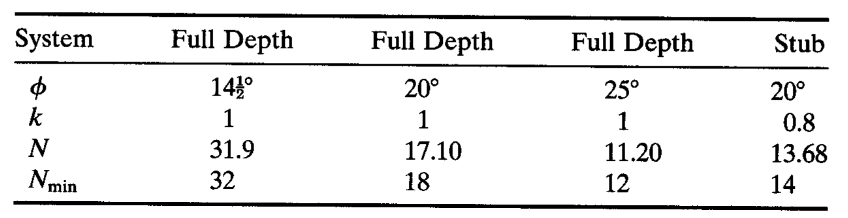
\includegraphics[width=.9\linewidth]{./images/minimum-number-of-teeth-to-avoid-interference-table.png}
\end{center}
\begin{itemize}
\item When a generation method is used in gear manufacturing, such as with a rack cutter, the interference problem will transform into an "undercutting" problem of removing materials in the interference regions, thus weakening the gear teeth.
\end{itemize}
\subsubsection{Rules on sizes of pinion and gear (or rack)}
\label{sec:org16c369b}
\begin{enumerate}
\item For a given gear (\(N_G\)) or rack, there exists a minimum number of teeth for the pinion, \(N_P^*\), such that there is no interference if the pinion tooth number \(N_P \ge N_P^2\), and that interference occurs if \(N_P < N_P^*\).
\item For a given pinion (\(N_P\)), there exists a maximum number of teeth for the gear, \(N_G^*\), such that there is no interference if the gear tooth number \(N_G \le N_G^*\), and that interference occurs if \(N_G > N_G^*\).
\end{enumerate}

Note that the "gear" and "pinion" refer to the larger and smaller parts of a (single-stage) gear transmission. Therefore, the relationship \(N_G > N_P\) always holds true.
\subsection{Idler}
\label{sec:orgaa4d2bc}
\begin{center}
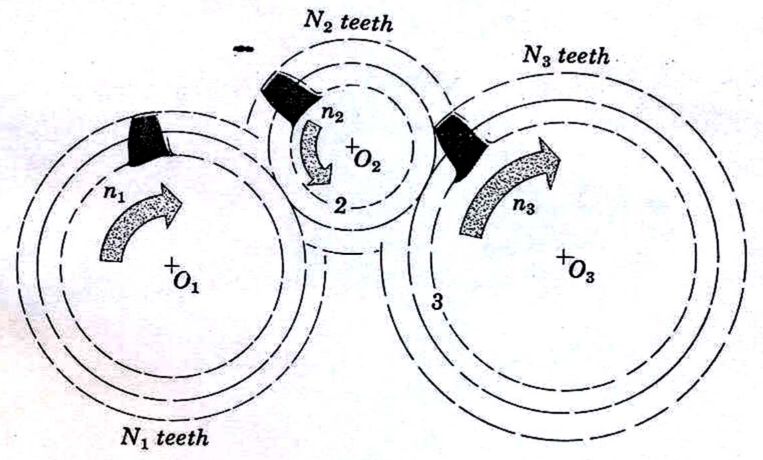
\includegraphics[width=.9\linewidth]{./images/idler-image.png}
\end{center}

For the equations below:
\begin{itemize}
\item \(n\) is the RPM of the gear
\item \(N\) is the number of teeth on the gear
\end{itemize}
\subsubsection{For gears 1 and 2}
\label{sec:orgb90f6ed}
\[\frac{n_2}{n_1} = - \frac{N_1}{N_2}\]
\subsubsection{For gears 2 and 3}
\label{sec:orgbe14874}
\[\frac{n_3}{n_2} = - \frac{N_2}{N_3}\]
\subsubsection{For gears 1 and 3}
\label{sec:orgc00c59f}
\[\frac{n_3}{n_1} = \left(\frac{n_3}{n_2}\right) \left(\frac{n_2}{n_1}\right) = \left(-\frac{N_2}{N_3} \right) \left(-\frac{N_1}{N_2} \right) = \frac{N_1}{N_3}\]
\subsection{Reversing gear box}
\label{sec:org0626d06}
\begin{center}
\includegraphics[width=.9\linewidth]{./images/reversing-gear-box-image.png}
\end{center}
\begin{itemize}
\item Two idlers are used between the input and output gears to change the direction of the output on the fly.
\item When the L-shaped arm is moved to the position shown in the right picture above, the input and output shafts will have opposite directions of rotation.
\end{itemize}
\subsection{Velocity ratio for spur gears (\(R\) or \(r_v\))}
\label{sec:orgbd09d42}
\begin{center}
\includegraphics[height=15em]{./images/double-stage-gear-reducer-image.png}
\end{center}
\[R \text{ or } r_v = \frac{|\omega_2|}{|\omega_1|} = \frac{|RPM_2|}{|RPM_1|} = \frac{r_1}{r_2} = \frac{d_{p1}}{d_{p2}} = \frac{N_1}{N_2}\]

Where:
\begin{itemize}
\item \(R\) or \(r_v\) is the velocity ratio
\item \(\omega\) is the angular velocity of the gear
\item \(RPM\) is the rotations per minute of the gear
\item \(r\) is the pitch radii of the gear
\item \(d_{p}\) is the pitch circle diameter of the gear
\item \(N\) is the number of teeth on the gear
\end{itemize}

\[r_v = \frac{\omega_2}{\omega_1} = - \frac{N_1}{N_2}\]

Where:
\begin{itemize}
\item \(R\) or \(r_v\) is the velocity ratio
\item \(\omega_2\) is the angular velocity of the second gear
\item \(\omega_1\) is the angular velocity of the first gear
\item \(N_1\) is the number of teeth on the first gear
\item \(N_2\) is the number of teeth on the second gear
\end{itemize}
\subsection{Output-to-input speed ratio}
\label{sec:org75040ee}
\begin{center}
\includegraphics[height=15em]{./images/double-stage-gear-reducer-image.png}
\end{center}
\begin{itemize}
\item The general relationship between the output rotational speed to the input rotational speed is given by:
\[\left|\frac{n_{output}}{n_{input}} \right| = \frac{\text{product of driving gear teeth}}{\text{product of driven gear teeth}}\]

Where:
\begin{itemize}
\item \(n_{output}\) is the rotations per minute of the output gear
\item \(n_{input}\) is the rotations per minute of the input gear
\end{itemize}

\item For the double-stage gear reducer above, it is:
\[\frac{n_4}{n_1} = \frac{N_1 N_3}{N_2 N_4}\]

Where:
\begin{itemize}
\item \(n_4\) is the rotations per minute of the gear 4
\item \(n_1\) is the rotations per minute of the gear 1
\item \(N_1\) is the number of teeth on gear 1
\item \(N_2\) is the number of teeth on gear 2
\item \(N_3\) is the number of teeth on gear 3
\item \(N_4\) is the number of teeth on gear 4
\end{itemize}
\end{itemize}
\subsection{Reverted gear train}
\label{sec:orgd063699}
\begin{center}
\includegraphics[width=.9\linewidth]{./images/reverted-gear-train-image.png}
\end{center}
In a reverted (or concentric) gear train, the input and output shaft have the same centreline.  \\

Geometric constraint:
\[r_1 + r_2 = r_3 + r_4\]

Where:
\begin{itemize}
\item \(r_1\) is the radius of gear 1 in the image above
\item \(r_2\) is the radius of gear 2 in the image above
\item \(r_3\) is the radius of gear 3 in the image above
\item \(r_4\) is the radius of gear 4 in the image above
\end{itemize}
\subsection{Gear reducer}
\label{sec:org7047e10}
One can ideally use two gears (single-stage gear transmission) to achieve the needed speed reduction, but due to size and cost constraints, multi-stage gear reducers are used.
\subsubsection{Double-stage gear reducer}
\label{sec:org443917d}
Velocity ratio:

\[\frac{n_4}{n_1} = \left(- \frac{N_1}{N_2} \right) \left(- \frac{N_3}{N_4} \right)\]

Where:
\begin{itemize}
\item \(N_1\) is the number of teeth on the first gear
\item \(N_2\) is the number of teeth on the second gear
\item \(N_3\) is the number of teeth on the third gear
\item \(N_4\) is the number of teeth on the third gear
\end{itemize}
\subsection{Speed ratio of planetary gear trains}
\label{sec:org10c8f0c}
\[\frac{n_{output} - n_c}{n_{input} - n_c} = \pm \frac{\text{product of driving gear teeth}}{\text{product of driven gear teeth}}\]

Where:
\begin{itemize}
\item \textbf{input} is an arbitrarily chosen starting point (not necessarily the real input)
\item \textbf{output} is an arbitrarily chosen ending point (not necessarily the real output)
\item \(n_{output}\) is the rotations per minute of the output gear
\item \(n_{c}\) is the rotations per minute of the carrier link
\item \(n_{input}\) is the rotations per minute of the input gear
\end{itemize}
\subsubsection{Example}
\label{sec:orged4bba4}
\begin{center}
\includegraphics[width=.9\linewidth]{./images/planetary-gear-train-kinematic-diagram.png}
\end{center}
\[\frac{n_R - n_C}{n_S - n_C} = \left(- \frac{N_S}{N_P} \right) \left( \frac{N_P}{N_R}\right)\]

Where:
\begin{itemize}
\item \(n_R\) is the rotations per minute of the ring gear
\item \(n_C\) is the rotations per minute of the planet carrier gear
\item \(n_S\) is the rotations per minute of the sun gear
\item \(N_S\) is the number of gear teeth on the sun gear
\item \(N_P\) is the number of gear teeth on the planet carrier gear
\item \(N_R\) is the number of gear teeth on the ring gear
\end{itemize}

 \newpage
\subsection{Velocity ratio for planetary gear trains}
\label{sec:org7719faf}
\begin{center}
\includegraphics[width=.9\linewidth]{./images/planetary-gear-train-kinematic-diagram.png}
\end{center}

Consider the sun gear (\(s\)) as the input and the ring gear (\(r\)) as the output (\(s \rightarrow p \rightarrow r\)) to set up the equation.

\[\frac{\omega_r - \omega_c}{\omega_s - \omega_c} = - \frac{N_s}{N_r}\]

Where:
\begin{itemize}
\item \(\omega_r\) is the angular velocity of the ring gear
\item \(\omega_c\) is the angular velocity of the planet carrier gear
\item \(\omega_r\) is the angular velocity of the ring gear
\item \(N_s\) is the number of teeth on the sun gear
\item \(N_r\) is the number of teeth on the ring gear
\end{itemize}
\subsubsection{Locked carrier}
\label{sec:org76b3c76}
A locked carrier means \(\omega_c = 0\), so:
\[\frac{\omega_r}{\omega_s} = - \frac{N_s}{N_r}\]
\subsubsection{Locked sun}
\label{sec:org4eb801e}
A locked sun means \(\omega_s = 0\), so:
\[\frac{\omega_r}{\omega_c} = 1 + \frac{N_s}{N_r}\]
\subsubsection{Locked ring}
\label{sec:org83852b4}
A locked ring means \(\omega_r = 0\), so:
\[\frac{\omega_s}{\omega_c} = 1 + \frac{N_r}{N_s}\]
\subsection{Scalar}
\label{sec:org8cfb009}
\begin{itemize}
\item A quantity with magnitude only, one-dimensional.
\item Examples:
\begin{itemize}
\item Temperature
\item Mass
\item Height
\item Pressure
\item Power
\end{itemize}
\end{itemize}
\subsection{Vector}
\label{sec:orge30dcee}
\begin{itemize}
\item A quantity with magnitude and direction, can be visualised using a line segment with an arrow, multidimensional.
\item Magnitude: Length of the line segment.
\item Direction: Direction of the arrow.
\item Examples:
\begin{itemize}
\item Force
\item Torque
\item Displacement
\item Velocity
\end{itemize}
\end{itemize}
\subsection{Unit vector}
\label{sec:orgf82a49f}
\begin{itemize}
\item A vector with a magnitude of 1.
\item Unit vectors along coordinate axes in 3D space:
\[\boldsymbol{i} = (1 \ 0 \ 0)\]
\[\boldsymbol{j} = (0 \ 1 \ 0)\]
\[\boldsymbol{k} = (0 \ 0 \ 1)\]
\end{itemize}
\subsection{Position vector}
\label{sec:org9ed5fdb}
\begin{itemize}
\item A position vector describes the location of a point \(P\) in space by drawing a line segment from the origin of the coordinate system to \(P\).
\item Magnitude: Length of the line segment.
\item Direction: Arrow from origin to \(P\).
\end{itemize}
\subsection{Vector components}
\label{sec:org28e540a}
\begin{itemize}
\item A vector can be expressed in terms of the summation of vectors along the coordinate axes (vector components).
\item Magnitude:
\[R = |\boldsymbol{R}| = \sqrt{R_x^2 + R_y^2 + R_z^2}\]
\item Unit vector (direction):
\[\boldsymbol{R}^u = \frac{\boldsymbol{R}}{R} = \frac{R_x}{R} \boldsymbol{i} \frac{R_y}{R} \boldsymbol{j} + \frac{R_z}{R} \boldsymbol{k}\]
\end{itemize}

\begin{center}
\includegraphics[height=20em]{./images/vector-components.png}
\end{center}
\subsection{2D planar vectors}
\label{sec:org2a012a1}
\begin{itemize}
\item Position vector of \(P\):
\[\boldsymbol{R} = \boldsymbol{i} R_x + R_y \boldsymbol{j} \equiv (R_x, R_y)\]
\[\boldsymbol{R} = (r \cos \theta) \boldsymbol{i} + (r \sin \theta) \boldsymbol{j}\]
\item Magnitude:
\[r = |\boldsymbol{R}| = \sqrt{R_x^2 + R_y^2}\]
\item Direction:
\[\boldsymbol{R}^u = \frac{\boldsymbol{R}}{r} = \cos \theta \boldsymbol{i} + \sin \theta \boldsymbol{j}\]
\end{itemize}

\begin{center}
\includegraphics[width=.9\linewidth]{./images/2d-planar-vectors.png}
\end{center}
\subsection{Motion}
\label{sec:org8ee8455}
\begin{itemize}
\item Motion is the way a rigid body moves in space.
\begin{itemize}
\item Most unrestrictive: 3D spatial motion, which is roughly 6 degrees-of-freedom (one body)

\begin{center}
\includegraphics[height=5em]{./images/3d-spatial-motion.png}
\end{center}
\item Restrictive: 2D planar motion, which is roughly 3 degrees-of-freedom (one body)

\begin{center}
\includegraphics[height=10em]{./images/2d-planar-motion.png}
\end{center}
\item Restrictive: 3D spherical motion, which is roughly 3 degrees-of-freedom (one body)

\begin{center}
\includegraphics[height=10em]{./images/3d-spherical-motion.png}
\end{center}
\end{itemize}
\item Any motion can be characterised by:
\begin{itemize}
\item Displacement with respect to a reference frame.
\item Velocity or speed of motion (displacement over time).
\item Acceleration of motion (velocity over time).
\end{itemize}
\end{itemize}
\subsection{Planar motion}
\label{sec:org11fbb37}
All points on the links of a mechanism is restricted to \textbf{one plane} or to \textbf{a set of parallel planes}. It is described and characterised by 2D vectors.
\begin{center}
\includegraphics[width=.9\linewidth]{./images/planar-motion.png}
\end{center}
\subsection{Purpose of position analysis}
\label{sec:org03f91a7}
\begin{itemize}
\item Given a fixed position or displacement of the input link, which can be an angle or a distance, depending on the type of joint or actuator.
\item Determine the position and orientation of all other links, including the output link.
\end{itemize}
\begin{center}
\includegraphics[width=.9\linewidth]{./images/position-analysis.png}
\end{center}
\subsection{Purpose of velocity analysis}
\label{sec:org0be1619}
\begin{itemize}
\item Given the velocity of the input link at a particular position.
\item Determine the velocities and angular velocities of all other links, including the output link.
\end{itemize}

\begin{center}
\includegraphics[width=.9\linewidth]{./images/velocity-analysis.png}
\end{center}
\subsection{Velocity of points}
\label{sec:org1400a5a}
\begin{itemize}
\item Velocity of a point in space is the time change of position with respect to a fixed reference frame. The direction is tangent to the trajectory, and the speed is the magnitude.
\[\boldsymbol{V} = \frac{d \boldsymbol{R}}{dt} = \dot{\boldsymbol{R}} = \dot{R}_x \boldsymbol{i} \dot{R}_y \boldsymbol{j} + \dot{R}_z \boldsymbol{k}\]
\item Relative velocity is the velocity between two points.
\begin{itemize}
\item Points \(A\) and \(B\) with \(V_A\) and \(V_B\).
\item Velocity of \(B\) relative \(A\) (\(V_{BA}\)):
\[\boldsymbol{V}_{BA} = \boldsymbol{V}_B - \boldsymbol{V}_A \text{ or } \boldsymbol{V}_B = \boldsymbol{V}_A + \boldsymbol{V}_{BA}\]
\item Take reference to the moving point.
\item Absolute velocity is the velocity with respect to a fixed point \(O\):
\[\boldsymbol{V}_{AO} = \boldsymbol{V}_A - \boldsymbol{V}_O = \boldsymbol{V}_A - 0 \equiv \boldsymbol{V}_A\]
\end{itemize}
\end{itemize}
\subsection{Planar rigid body motion}
\label{sec:org6583246}
\begin{itemize}
\item Fixed point, pure rotation, one point has no velocity.
\item Pure translation, all points have the same velocity.
\item General rotation and translation, the velocity different for every point.
\end{itemize}
\subsection{Velocity of rigid body}
\label{sec:org2629d29}
\begin{itemize}
\item Angular velocity for a body:
\begin{itemize}
\item Scalar: Time changes the angular position of a body.
\[\omega = \lim_{N \rightarrow 0} \frac{\delta \theta}{\Delta t} = \frac{d \theta}{dt}\]
\[\boldsymbol{\omega} = \omega_x \boldsymbol{i} + \omega_y \boldsymbol{j} + \omega_z \boldsymbol{k}\]
\item Vector: Showing rotation axis and speed:
\[\boldsymbol{\omega} = \omega \boldsymbol{k}\]
\end{itemize}
\item Right-hand rule for \(\omega\):
\begin{itemize}
\item Counter-clockwise is positive
\item Clockwise is negative
\end{itemize}
\item Velocity of points on the rotating body:
\[\boldsymbol{V}_A = \boldsymbol{\omega} \times \boldsymbol{r}_A\]
\[\text{For planar object: } v_A = \omega \cdot r_A\]
\end{itemize}

 \newpage
\subsection{Relative velocity of rigid body}
\label{sec:orgdce79c4}
\begin{itemize}
\item Use graphical construction of the \textbf{velocity polygon} formed by \textbf{velocities of points on link members} to find angular velocity of link and linear velocity of other points on link.
\item \textbf{Each link member} can form one relative velocity equation.
\end{itemize}
\[\boldsymbol{V}_B = \boldsymbol{V}_A + \boldsymbol{V}_{BA}\]
\[\boldsymbol{V}_{BA} = \boldsymbol{\omega} \times \boldsymbol{r}_{BA}\]

\begin{center}
\includegraphics[width=.9\linewidth]{./images/relative-velocity-of-rigid-body.png}
\end{center}

 \newpage
\subsection{Velocity image}
\label{sec:org23deeec}
\begin{itemize}
\item It is a \textbf{similar-shaped figure in the velocity diagram} to the original link (object).
\begin{itemize}
\item The line is mapped to a line, a triangle is mapped to a triangle, and a circle is mapped to a circle, etc.
\item The \textbf{orientation and size} will be different.
\end{itemize}
\begin{center}
\includegraphics[width=.9\linewidth]{./images/velocity-image-comparison.png}
\end{center}

\item It is used to determine the velocity of points on linkages not on the joint centres, like point \(D\) in the image below.
\begin{center}
\includegraphics[width=.9\linewidth]{./images/velocity-image-diagram.png}
\end{center}
\end{itemize}

 \newpage
\subsubsection{Example}
\label{sec:org26e6b76}
\begin{itemize}
\item \(DBCD\) is a rigid body, and \(Dbcd\) are points in a velocity diagram.
\item \(Dbcd\) is the velocity image of \(DBCD\), i.e. \(DBCD\) is similar to \(Dbcd\).
\begin{itemize}
\item \(Dbcd\) is \(DBCD\) rotated \(\qty{90}{\degree}\) counter-clockwise.
\item It is magnified by a factor of \(\omega\).
\end{itemize}
\item The edges of the velocity image are relative velocity.
\end{itemize}

\[\boldsymbol{V}_{CB} = \omega \times \boldsymbol{r}_{CB} \sim \vec{bc}\]
\[\boldsymbol{V}_{DC} = \omega \times \boldsymbol{r}_{DC} \sim \vec{cd}\]
\[\boldsymbol{V}_{BD} = \omega \times \boldsymbol{r}_{BD} \sim \vec{bd}\]

\begin{center}
\includegraphics[width=.9\linewidth]{./images/velocity-image-example.png}
\end{center}

 \newpage
\subsubsection{Velocity image of collinear points}
\label{sec:org981637e}
\begin{itemize}
\item Velocity image of link \(BC\) is a straight line segment.
\item Velocity of points on link can be obtained proportionally.
\end{itemize}

\begin{center}
\includegraphics[height=20em]{./images/velocity-image-of-collinear-points-mechanism.png}
\end{center}

\begin{center}
\includegraphics[height=20em]{./images/velocity-image-of-collinear-points-polygon.png}
\end{center}
\subsection{Purpose of acceleration analysis}
\label{sec:org22485f0}
\begin{itemize}
\item Given the acceleration of the input link at a particular position.
\item Determine the accelerations and angular accelerations of all other links, including the output link.
\end{itemize}
\subsection{Acceleration of points}
\label{sec:org3048385}
\begin{itemize}
\item The acceleration of a point in space is the time change of velocity with respect to the fixed reference frame:
\[\boldsymbol{A} = \frac{d \boldsymbol{V}}{dt} \ddot{\boldsymbol{R}} \ddot{R}_x \boldsymbol{i} + \ddot{R}_y + \boldsymbol{j} + \ddot{R}_z \boldsymbol{k}\]
\item Relative acceleration is the acceleration between two points.
\begin{itemize}
\item Points \(A\) and \(B\) with \(A_A\) and \(A_B\).
\item Acceleration of \(B\) relative to \(A\) (\(A_{BA}\)):
\[\boldsymbol{A}_{BA} = \boldsymbol{A}_B - \boldsymbol{A}_A\]
\[\boldsymbol{A}_{B} = \boldsymbol{A}_A - \boldsymbol{A}_{BA}\]
\item Take reference to the moving point.
\item Absolute acceleration is the acceleration taken with reference toa  fixed point \(O\):
\[\boldsymbol{A}_{AO} = \boldsymbol{A}_A - \boldsymbol{A}_O = \boldsymbol{A}_A - 0 \equiv \boldsymbol{A}_A\]
\end{itemize}
\end{itemize}
\subsection{Angular acceleration of a rigid body}
\label{sec:org950f7aa}
\begin{itemize}
\item Angular acceleration for a body:
\begin{itemize}
\item Scalar: Time changes the angular velocity of a body:
\[\alpha = \lim_{N \rightarrow 0} \frac{\delta \omega}{\Delta t} = \frac{d \omega}{dt} = \ddot{\theta}\]
\[\boldsymbol{\alpha} = \alpha_x \boldsymbol{i} + \alpha_y \boldsymbol{j} + \alpha_z \boldsymbol{k}\]
\item Vector: Showing rotation axis and speed:
\[\boldsymbol{\alpha} = \omega \boldsymbol{k}\]
\end{itemize}
\item Right-hand rule for \(\alpha\):
\begin{itemize}
\item Counter-clockwise is positive
\item Clockwise is negative
\end{itemize}
\end{itemize}
\subsection{Motion of rigid body at fixed point}
\label{sec:org84f766c}
\begin{itemize}
\item Velocity of point on rigid body rotating about a fixed axis:
\[\boldsymbol{V} = \dot{\boldsymbol{R}} = \boldsymbol{\omega} \times \boldsymbol{R}\]
\item Acceleration of point:
\[\ddot{\boldsymbol{V}} = \ddot{\boldsymbol{\omega}} \times \boldsymbol{R} + \boldsymbol{\omega} \times \ddot{\boldsymbol{R}}\]
\[\ddot{\boldsymbol{A}} = \ddot{\boldsymbol{\alpha}} \times \boldsymbol{R} + \boldsymbol{\omega} \times (\omega \times \ddot{\boldsymbol{R}}) = \boldsymbol{A}^t + \boldsymbol{A}^n\]
\item Tangential acceleration is the acceleration tangent to the path and perpendicular to \(R\).
\[\boldsymbol{A}^t = \boldsymbol{\alpha} \times \boldsymbol{R}\]
\item Normal or radian acceleration is the acceleration parallel to \(R\), pointing towards \(O\).
\[\boldsymbol{A}^n = \omega \times (\omega \times \boldsymbol{R})\]
\item For planar motion:
\[A^t = \alpha R\]
\[A^n = \omega^2 R = \frac{V^2}{R}\]
\[\text{Total magnitude: } A = \sqrt{(A^n)^2 + (A^t)^2}\]
\end{itemize}

 \newpage
\subsection{Relative accelerations}
\label{sec:org7786ed9}
\begin{itemize}
\item Differentiate relative velocity equation:
\[\boldsymbol{V}_B = \boldsymbol{V}_A + \boldsymbol{\omega} \times \boldsymbol{r}_{BA}\]
\item To form the relative acceleration equation:
\begin{align*}
\boldsymbol{A}_B &= \boldsymbol{A}_A + \boldsymbol{\omega} \times (\boldsymbol{\omega} \times \boldsymbol{r}_{BA}) + \boldsymbol{\alpha} \times \boldsymbol{r}_{BA} \\
&= \boldsymbol{A}_A - \omega^2 \boldsymbol{r}_{BA} + \boldsymbol{\alpha} \times \boldsymbol{r}_{BA} \\
&= \boldsymbol{A}_A + \boldsymbol{A}_{BA}^t + \boldsymbol{A}_{BA}^n
\end{align*}
\[A_{BA}^t = \boldsymbol{\alpha} \times \boldsymbol{r}_{BA}\]
\[A_{BA}^n = \omega^2 \boldsymbol{r}_{BA}\]

Where:
\begin{itemize}
\item \(\boldsymbol{A}_A, \boldsymbol{A}_B\) are the absolute accelerations of point \(A\) and \(B\) relative to the fixed frame.
\item \(\boldsymbol{A}_{BA}^t\) is the tangential acceleration of \(B\) relative to \(A\).
\item \(\boldsymbol{A}_{BA}^n\) is the normal acceleration of \(B\) relative to \(A\), \(\boldsymbol{A}_{BA}^n \parallel \boldsymbol{r}_{BA}\)
\item \(\boldsymbol{r}_{BA}\) is the position vector of \(B\) relative to \(A\), \(\boldsymbol{A}_{BA}^t \perp \boldsymbol{r}_{BA}\)
\item \(\boldsymbol{\alpha}\) is the angular acceleration of the body relative to the fixed frame.
\end{itemize}
\end{itemize}
\subsection{Acceleration at revolute joints}
\label{sec:org1b7e313}
\[\boldsymbol{A}_{B1} = \boldsymbol{A}_{B2}\]

\begin{center}
\includegraphics[height=15em]{./images/acceleration-at-revolute-joints.png}
\end{center}
\subsection{Acceleration at prismatic joints}
\label{sec:orgc61eabe}
\[\boldsymbol{V}_{B1} \ne \boldsymbol{V}_{B2}\]
\[\boldsymbol{A}_{B1} \ne \boldsymbol{A}_{B2}\]
\[V_{B2B1} \parallel A_{B1B2} \parallel \text{Direction of travel}\]

\begin{center}
\includegraphics[width=.9\linewidth]{./images/acceleration-at-prismatic-joints.png}
\end{center}

 \newpage
\subsection{Acceleration image}
\label{sec:org7b28f59}
\begin{itemize}
\item A \textbf{similar-shaped} figure in the acceleration diagram to the original link (object).
\begin{itemize}
\item Orientation and size are different from the link and its velocity image.
\end{itemize}
\begin{center}
\includegraphics[width=.9\linewidth]{./images/acceleration-image-comparison.png}
\end{center}
\item It is used to determine the acceleration of points on linkages not on the joint centres, e.g. point \(D\) in the image below.
\begin{center}
\includegraphics[width=.9\linewidth]{./images/velocity-image-diagram.png}
\end{center}
\end{itemize}

 \newpage
\subsubsection{Example}
\label{sec:orgc416a21}
\begin{itemize}
\item \(DBCD\) is a rigid body, and \(Db'c'd'\) are points an acceleration diagram.
\item \(Db'c'd'\) is the velocity image of \(DBCD\), i.e. \(DBCD\) is similar to \(Db'c'd'\).
\begin{itemize}
\item \(Db'c'd'\) is \(DBCD\) rotated \(\theta = \pi - \tan^{-1} \left(\frac{\alpha}{\omega^2} \right)\)
\item It is magnified by a factor of \(\sqrt{\omega^4 + \alpha^2}\).
\end{itemize}
\item Order of the points remains:
\begin{itemize}
\item Links: \(B \rightarrow C \rightarrow D\)
\item Velocity polygon: \(b \rightarrow c \rightarrow d\)
\item Acceleration polygon: \(b' \rightarrow c' \rightarrow d'\)
\item When one side of the acceleration image is found, e.g. \(\boldsymbol{A}_{BC}\), the orientation of the acceleration image can be determined.
\end{itemize}
\end{itemize}
\subsubsection{Acceleration image of collinear points}
\label{sec:org99f6d3f}
\begin{itemize}
\item Acceleration image of link \(BC\) to \(a\) is a straight line segment.
\item Acceleration of points on the link can be obtained proportionally from the acceleration polygon.
\end{itemize}

\begin{center}
\includegraphics[height=10em]{./images/acceleration-image-of-collinear-points-mechanism.png}
\end{center}
\begin{center}
\includegraphics[height=10em]{./images/acceleration-image-of-collinear-points-polygon.png}
\end{center}
\subsection{Jerk (\(J\))}
\label{sec:org77c4744}
\begin{itemize}
\item Jerk (\(J\)) is defined as the third-order derivative of the displacement with respect to time.
\[J = \frac{d^3 s}{dt^3}\]
\item It is equal to the derivative of the acceleration.
\[J = \frac{da}{dt}\]
\item Jerk is an important variable to characterise the smoothness of motion of an object or a mechanism.
\item In addition to a finite acceleration, a finite jerk is desirable for the smooth operation of a cam-follower system.
\item For high speed operation of cams, displacement, velocity and acceleration must be continuous, and jerk must be finite.
\end{itemize}
\subsection{Newton's first law}
\label{sec:orgb8e98ac}
Every object remains at rest or moves with constant velocity, unless an unbalanced force acts on it.

 \newpage
\subsection{Newton's second law}
\label{sec:org3003a66}
And object that has an unbalanced force, has an acceleration that is:
\begin{enumerate}
\item Proportional to the force
\item In the direction of the force
\item Inversely proportional to the mass of the object
\end{enumerate}

For translation:
\[\sum \vec{F}_i = m \vec{a}\]

In two-dimensions, two scalar equations can be created from the above equation:
\[\sum F_{ix} = m a_x\]
\[\sum F_{iy} = m a_y\]

For rotation about a fixed point:
\[\tau = \sum M_i = I \alpha\]

\begin{center}
\includegraphics[height=10em]{./images/rotation-about-a-fixed-point-diagram.png}
\end{center}

Where:
\begin{itemize}
\item \(\sum \vec{F}\) is the sum of the forces acting on the object
\item \(m\) is the mass of the object
\item \(\vec{a}\) is the acceleration of the object
\item \(\tau\) is the torque on the object
\item \(\sum M_i\) is the sum of the moments on the object
\item \(I\) is the moment of inertia about a fixed point
\item \(\alpha\) is the angular acceleration of the object
\end{itemize}

 \newpage
\subsubsection{General planar motion}
\label{sec:orgac58dab}
\begin{center}
\includegraphics[height=20em]{./images/general-planar-motion-diagram.png}
\end{center}

Translation of the centre of gravity (CG):
\[\sum \vec{F}_j = m \vec{a}_G\]

Rotation about the centre of gravity (CG):
\[\sum M_{jG} = I_G \alpha\]

Where:
\begin{itemize}
\item \(\sum \vec{F}_j\) is the sum of the forces acting on the object
\item \(m\) is the mass of the object
\item \(_G\) denotes the centre of mass of the object
\item \(\vec{a}_G\) is the acceleration of the centre of mass of the object
\item \(\sum M_{jG}\) is the sum of moments acting about the centre of mass of the object
\item \(I_G\) is the moment of inertia of the object about \(G\)
\item \(\alpha\) is the angular acceleration of the object
\end{itemize}
\subsection{Newton's third law}
\label{sec:orga1f73cf}
For every action, there is an equal and opposite reaction.
\subsection{Statics}
\label{sec:orgdd21760}
Statics deals with the equilibrium of bodies that are either \textbf{at rest} or move with a \textbf{constant velocity}.
\subsection{Dynamics}
\label{sec:org8a91321}
Dynamics deals with the \textbf{accelerated motion} of bodies.
\subsection{Kinematics}
\label{sec:org48777f2}
Kinematics is the study of motion, \textbf{quite apart from the forces} which produce that motion. More particularly, it is the study of position, displacement, rotation, velocity, and acceleration.

 \newpage
\subsection{Forces and moments}
\label{sec:org8c15bdc}
\begin{itemize}
\item Forces and moments (couples) are vectors.
\[\vec{F} = F_x \vec{i} + F_y \vec{j} + F_z \vec{k}\]
\item There are \textbf{three} components in the x, y and z directions in the Cartesian coordinate system.
\item \(\boldsymbol{\vec{r}}\) is a position vector from a \textbf{reference point} to the point where a force is applied.
\item A \textbf{reference point} is needed to define \textbf{the moment} but not for the force.
\begin{align*}
\vec{M} = \vec{r} \times \vec{F} &= \begin{vmatrix}
\vec{i} & \vec{j} & \vec{k} \\
r_x & r_y & r_z \\
F_x & F_y F_z \\
\end{vmatrix} \\
&= (r_y F_z - r_z F_y) \vec{i} + (r_z F_x - r_x F_z) \vec{j} + (r_x F_y - r_y F_x) \vec{k}
\end{align*}
\end{itemize}

\begin{center}
\includegraphics[height=20em]{./images/forces-and-moments.png}
\end{center}

 \newpage
\subsection{Free-body diagram}
\label{sec:orgfc6fd4a}
\begin{itemize}
\item A free-body diagram is a sketch or drawing of part or all of a system, isolated to determine the nature of the forces acting on the body.
\item An isolated part is separated from the system.
\item All external forces and moments on the part are depicted.
\item Static or dynamic analysis is carried out.
\end{itemize}
\subsubsection{Examples}
\label{sec:org8aa16bd}
\begin{enumerate}
\item A four-bar linkage.
\begin{center}
\includegraphics[height=15em]{./images/free-body-diagram-four-bar-linkage.png}
\end{center}
\item Free-body diagram of the three moving links.
\begin{center}
\includegraphics[height=15em]{./images/free-body-diagram-three-moving-links.png}
\end{center}
\item Free-body diagram of two connected links.
\begin{center}
\includegraphics[height=15em]{./images/free-body-diagram-two-connected-links.png}
\end{center}
\item Free-body diagram of a single link.
\begin{center}
\includegraphics[width=.9\linewidth]{./images/free-body-diagram-single-link.png}
\end{center}
\item Free-body diagram of part of a link.
\begin{center}
\includegraphics[width=.9\linewidth]{./images/free-body-diagram-part-of-a-link.png}
\end{center}
\end{enumerate}
\subsection{Static equilibrium}
\label{sec:org74d3ad8}
If a system is in static equilibrium, i.e. \(\vec{a} = 0\) and \(\alpha = 0\), then:
\[\sum \vec{F} = 0 \qquad \text{Resultant force} = 0\]
\[\sum \vec{M}_G = 0 \qquad \text{Resultant moment} = 0\]
\subsection{Graphical force analysis}
\label{sec:orgfd0bb1c}
\begin{itemize}
\item Graphical force analysis employs \textbf{scaled free-body diagrmas} and \textbf{vector graphics} in the detmination of unknown machine forces.
\item The graphical approach is best suited for planat force systems.
\end{itemize}
\subsection{Special free-body diagrams}
\label{sec:orgfa2cd9a}
\begin{itemize}
\item Two-force member
\item Three-force member
\item Two-force and a couple member
\item N-force members \(N > 3\) are not of much practical interest
\end{itemize}
\subsubsection{Two-force member}
\label{sec:orgdea1235}
When a link is subjected to only two forces:
\begin{itemize}
\item We refer to the link as a "2-force member".
\item The forces must be \textbf{axial} (along the axis).
\item The 2 forces must be \textbf{equal and opposite}.
\item The two external forces are \textbf{equal, opposite and co-linear aligned with the link}.
\end{itemize}

\begin{center}
\includegraphics[width=.9\linewidth]{./images/free-body-diagram-two-force-member.png}
\end{center}
\subsubsection{Three-force member}
\label{sec:orgc1b4577}
A member subjected to three forces is in equilibrium if and only if:
\begin{itemize}
\item The resultant of the three forces is zero.
\item The action lines of th forces all intersect at the same point.
\item Force equilibrium condition states that:
\[F_1 + F_2 + F_3 = 0\]

Three forces form a closed vector loop, a force polygon:
\begin{center}
\includegraphics[width=.9\linewidth]{./images/three-force-member-force-polygon.png}
\end{center}

\item All three external forces are \textbf{co-centred} and form a \textbf{closed triangle}.
\end{itemize}

\begin{center}
\includegraphics[width=.9\linewidth]{./images/free-body-diagram-three-force-member.png}
\end{center}
\subsubsection{Two-force and a couple member}
\label{sec:org4e59eb3}
Two external forces are \textbf{parallel, opposite and equal}.
\begin{center}
\includegraphics[width=.9\linewidth]{./images/two-force-and-a-couple-member-diagram.png}
\end{center}
\subsection{Friction}
\label{sec:orge88f68a}
\begin{itemize}
\item Friction is everywhere in our daily life and in machines.
\item Friction can dissipate energy by converting mechanical work into heat.
\item It reduces the efficiency of a machine.
\end{itemize}

 \newpage
\subsection{Coulomb friction}
\label{sec:orge378e2a}
\begin{itemize}
\item A friction is called \textbf{Coulomb Friction} when it is linearly proportional to the normal contact force.
\[f = \mu N\]

Where:
\begin{itemize}
\item \(f\) is the friction
\item \(\mu\) is the coefficient of friction
\item \(N\) is the normal contact force
\end{itemize}

\item The direction of friction is opposite to the \textbf{relative velocity} between two contact surfaces.
\end{itemize}

\begin{center}
\includegraphics[height=15em]{./images/coulomb-friction-diagram.png}
\end{center}

 \newpage
\subsection{D'Alembert's principle}
\label{sec:orgf2a61c0}

\begin{center}
\includegraphics[width=.9\linewidth]{./images/newtons-law-diagram.png}
\end{center}
\begin{center}
\includegraphics[width=.9\linewidth]{./images/d-alemberts-principle-diagram.png}
\end{center}
\subsubsection{Force equation}
\label{sec:org7f9e772}
Newton's second law:
\[\sum \vec{F}_j = m \vec{a}_G\]
\[\sum \vec{F}_j - m \vec{a}_G = 0\]

Defining inertial force to be:
\[\vec{F}_I = - m \vec{a}_G\]

We have:
\[\sum \vec{F}_j + \vec{F}_I = 0\]
\[\sum \vec{F}_i = 0\]

Imaginary (mathematic) "static" equilibrium state with an additional inertial force:
\[\vec{F}_I = - m \vec{a}_G\]
\subsubsection{Moment equation}
\label{sec:org9847cab}
Newton's second law:
\[\sum M_{jG} = I_G \alpha\]
\[\sum M_{jG} - I_G \alpha = 0\]

Defining inertial moment to be:
\[C_I = - I_G \alpha\]

We have:
\[M_{jG} + C_I = 0\]
\[\sum M_i = 0\]

Imaginary (mathematic) "static" equilibrium state with an additional inertial moment:
\[C_I = - I_G \alpha\]
\subsubsection{Link example}
\label{sec:org4bdef8d}
Newton's second law:
\begin{center}
\includegraphics[height=15em]{./images/newtons-law-link-example-diagram.png}
\end{center}

Dynamic problem:
\[\sum \vec{F}_j = m \vec{a}_G\]
\[\sum M_{jG} = I_G \alpha\]

D'Alembert's principle:
\begin{center}
\includegraphics[height=15em]{./images/d-alemberts-principle-link-example-diagram.png}
\end{center}
\[\sum \vec{F}_j = 0\]
\[\sum \vec{M}_j = 0\]
\subsubsection{Convention for inertial force and moment}
\label{sec:orge090413}
For motion:
\begin{center}
\includegraphics[width=.9\linewidth]{./images/d-alemberts-principle-convention-for-motion-diagram.png}
\end{center}

For inertial force and moment:
\begin{center}
\includegraphics[width=.9\linewidth]{./images/d-alemberts-principle-convention-for-inertial-force-and-moment-diagram.png}
\end{center}

 \newpage
\subsection{Mass moment of inertia}
\label{sec:orga1431ee}
\[I_G = \int r^2 \rho \, dV\]

Where:
\begin{itemize}
\item \(I_G\) is the moment of inertia about the centre of the body
\item \(\rho\) is the density of the body
\item \(r\) is the distance from the centre of mass to an arbitrary point inside the body.
\end{itemize}
\subsubsection{Slender rod}
\label{sec:org5527606}
\begin{center}
\includegraphics[width=.9\linewidth]{./images/moment-of-inertia-slender-rod-diagram.png}
\end{center}
\[I_G = \frac{1}{12} mL^2\]
\[I_O = \frac{1}{3} mL^2\]
\subsubsection{Disk or cylinder}
\label{sec:orga430327}
\begin{center}
\includegraphics[width=.9\linewidth]{./images/moment-of-inertia-cylinder-or-disk-diagram.png}
\end{center}
\[I_G = \frac{1}{2} mr^2\]
\subsubsection{Rectangular plate}
\label{sec:orgcb95ee4}
\begin{center}
\includegraphics[width=.9\linewidth]{./images/moment-of-inertia-rectangular-plate-diagram.png}
\end{center}
\[I_G = \frac{1}{12} m (a^2 + b^2)\]
\subsubsection{Ring}
\label{sec:org6729b00}
\begin{center}
\includegraphics[width=.9\linewidth]{./images/moment-of-inertia-ring-diagram.png}
\end{center}
\[I_G = \frac{1}{2} m (r_1^2 + r_2^2)\]
\subsubsection{Thin ring}
\label{sec:org0a81050}
\begin{center}
\includegraphics[width=.9\linewidth]{./images/moment-of-inertia-thin-ring-diagram.png}
\end{center}
\[I_G = mr^2\]
\subsubsection{Semicircular plate}
\label{sec:org2af66f2}
\begin{center}
\includegraphics[width=.9\linewidth]{./images/moment-of-inertia-semicircular-plate-diagram.png}
\end{center}
\[I_G = \frac{1}{2} mr^2\]
\[I_O = \frac{1}{2} mr^2 - mh^2\]
\[h = \frac{4r}{3 \pi}\]

 \newpage
\subsection{Parallel axis theorem}
\label{sec:orgf6275d5}
For the mass moment of inertia being taken about a point \(A\) other than the centre of mass \(G\), we can derive the mass moment of inertia using the following parallel axis theorem:
\[I_A = I_G + m \left| \vec{r}_{AG} \right|^2\]

Where:
\begin{itemize}
\item \(I_A\) is the moment of inertia taken about an arbitrary point \(A\)
\item \(I_G\) is the moment of inertia taken about the centre of mass \(G\)
\item \(m\) is the mass of the object
\item \(\vec{r}_{AG}\) is the position vector from point \(A\) to the centre of mass \(G\)
\end{itemize}

\begin{center}
\includegraphics[width=.9\linewidth]{./images/parallel-axis-theorem-diagram.png}
\end{center}

 \newpage
\subsubsection{Example}
\label{sec:orge91c811}
\begin{center}
\includegraphics[height=10em]{./images/moment-of-inertia-example-diagram.png}
\end{center}

Determine the mass moment of inertia of the assemly about its centre of mass \(G\) and point \(C\). The moment so finertia of the disk and the rod about their mass centres \(A\) and \(B\) are known to be \(I_A = \frac{1}{2} m_D r^2\) and \(I_B = \frac{1}{12} m_r L^2\) respectively.

\begin{itemize}
\item Centre of mass:
Using point \(A\) as the origin, the centre of mass can be located as:
\[r_{AG} = \frac{m_D r_{AA} + m_R + r_{AB}}{m_R + m_D}, \qquad r_{AA} = 0\]
\[r_{AG} = \qty{0.15}{m}\]

\item Mass moment of inertia about \(G\):
Using the parallel axis theorem, the moment of inertia can be calculated as follows:
\begin{align*}
\text{Disk: } I_G^{disk} &= I_A + m_D r^2_{AG} \\
&= \frac{1}{2} (5) (0.1)^2 \\
&= \qty{0.1375}{kg.m^2} \\
\text{Rod: } I_G^{rod} &= I_B + m_D r^2_{BG} \\
&= \frac{1}{2} (3) (0.6)^2 + 3(0.25)^2 \\
&= \qty{0.2775}{kg.m^2} \\
I_G &= I_G^{disk} + I_G^{rod} \\
&= \qty{0.415}{kg.m^2}
\end{align*}

\item Mass moment of inertia about \(C\):
Similarly, we have:
\begin{align*}
I_C &= I_C^{disk} + I_C^{rod} \\
&= I_G + (m_D + m_R) r_{CG}^2 \\
&= \qty{2.835}{kg.m^2}
\end{align*}
\end{itemize}

 \newpage
\section{Types of gears}
\label{sec:org1d10211}

\subsection{Spur gears and helical gears}
\label{sec:org7a2af47}
\begin{center}
\includegraphics[width=.9\linewidth]{./images/spur-and-helical-gears.png}
\end{center}
\begin{itemize}
\item Spur and helical gears are normally used when the driver and the follower shafts are parallel. Helical gears provide smoother, quieter, and less-shock operation.
\item The smaller gear in a pair of meshing gears is called a \textbf{pinion}.
\end{itemize}
\subsection{Pinion and rack}
\label{sec:org31c4449}
\begin{center}
\includegraphics[width=.9\linewidth]{./images/pinion-and-rack.png}
\end{center}
\begin{itemize}
\item A rack is a straight bar with gear teeth, and may be considered as a spur gear with an infinite radius.
\end{itemize}
\subsection{Bevel gears}
\label{sec:orgd55531f}
\begin{center}
\includegraphics[width=.9\linewidth]{./images/straight-and-spiral-bevel-gears.png}
\end{center}
\begin{itemize}
\item Bevel gears are used when the driver and driven shafts' centreline intersect.
\end{itemize}
\subsection{Worm gears}
\label{sec:orge06b919}
\begin{center}
\includegraphics[width=.9\linewidth]{./images/worm-gears.png}
\end{center}
\begin{itemize}
\item Worm gears are used when the driver and driven shaft centreline are at 90 degrees.
\item Worm gear (on the left) is a special helical gear (on the right).
\end{itemize}
\section{Module pitch tooth dimensions}
\label{sec:org801e734}
\begin{center}
\includegraphics[width=.9\linewidth]{./images/module-pitch-tooth-dimensions.png}
\end{center}
\section{Contact geometry for a pair of meshing gears}
\label{sec:orgb99e163}
\begin{center}
\includegraphics[width=.9\linewidth]{./images/contact-geometry-for-a-pair-of-meshing-gears.png}
\end{center}
\section{Gear standards}
\label{sec:org77259cb}
\begin{center}
\includegraphics[width=.9\linewidth]{./images/gear-standards-table.png}
\end{center}

 \newpage
\section{How to analyse planetary gear trains (PGT).}
\label{sec:org3793ed5}
\begin{center}
\includegraphics[width=.9\linewidth]{./images/planetary-gear-train-simplified-diagram.png}
\end{center}
"Hold" the carrier link (\(c\)), which is fixed, and rotate gear 1.

\[\frac{n_{2/c}}{n_{1/c}} = - \frac{N_1}{N_2}\]

Where:
\begin{itemize}
\item \(n_{2/c}\) is the rotations per minute of gear 2 relative to the carrier link
\item \(n_{1/c}\) is the rotations per minute of gear 1 relative to the carrier link
\item \(N_1\) is the number of teeth on gear 1
\item \(N_2\) is the number of teeth on gear 2
\end{itemize}

 \newpage
\subsection{Kinematic diagram}
\label{sec:org271b3a6}
\begin{center}
\includegraphics[width=.9\linewidth]{./images/planetary-gear-train-kinematic-diagram.png}
\end{center}

Note that the carrier link rotates independently of the sun gear.
\subsection{Levai variations of planetary gear trains}
\label{sec:orgd57231d}
\begin{center}
\includegraphics[width=.9\linewidth]{./images/levai-variations-of-planetary-gear-trains.png}
\end{center}

 \newpage
\section{Getting the velocity ratio of a gear chain}
\label{sec:org2ba2c74}
The velocity ratio a gear chain is generally:
\[\frac{\text{Target gear velocity}}{\text{Driving gear velocity}} = \frac{\text{Number of driving gear teeth}}{\text{Number of driven gear teeth}}\]

\begin{itemize}
\item If there is a carrier, or the gear chain is a planetary gear chain, the velocity ratio will be relative to the carrier speed, so the velocity ratio equation must subtract the carrier speed term, \(- n_c\).
\item When the gear interaction is between an external gear and another external gear, the gear teeth ratio must be \textbf{negative (-)}.
\item When the gear interaction is between an external gear and another internal gear, the gear teeth ratio must be \textbf{positive (+)}.
\end{itemize}

 \newpage
\section{Vector algebra}
\label{sec:org33b6696}
Let:
\[\boldsymbol{A} = A_x \boldsymbol{i} A_y \boldsymbol{j} + A_z \boldsymbol{k}\]
\[\boldsymbol{B} = B_x \boldsymbol{i} B_y \boldsymbol{j} + B_z \boldsymbol{k}\]
\subsection{Equivalence}
\label{sec:org7bd0be7}
\[\boldsymbol{A} = \boldsymbol{B} \Leftrightarrow A_x = B_x, A_y = B_y, A_z = B_z\]
\subsection{Addition}
\label{sec:orga506492}
\[\boldsymbol{C} = \boldsymbol{A} + \boldsymbol{B} \Leftrightarrow \boldsymbol{C} = (A_x + B_x) \boldsymbol{i} + (A_y + B_y) \boldsymbol{j} + (A_z + B_z) \boldsymbol{k}\]
\subsection{Subtraction}
\label{sec:org453d20a}
\[\boldsymbol{D} = \boldsymbol{A} - \boldsymbol{B} \Leftrightarrow \boldsymbol{D} = (A_x - B_x) \boldsymbol{i} + (A_y - B_y) \boldsymbol{j} + (A_z - B_z) \boldsymbol{k}\]
\subsection{Scalar multiplication}
\label{sec:org7ef2e71}
\[m \boldsymbol{A} = mA_x \boldsymbol{i} + mA_y \boldsymbol{j} + mA_z \boldsymbol{k}\]
\subsection{Cross product}
\label{sec:org4c4dc6c}
\[\boldsymbol{A} \times \boldsymbol{B} = (A_y B_z - A_z B_y) \boldsymbol{i} + (A_z B_x - A_x B_z) \boldsymbol{j} + (A_x B_y - A_y B_x) \boldsymbol{k}\]
\subsection{Inner (dot) product}
\label{sec:org3183168}
\[\boldsymbol{A} \cdot \boldsymbol{B} = A_x B_x + A_y B_y + A_z + B_z\]
\subsection{Vector derivatives}
\label{sec:orga74b4ec}
\[\frac{d}{dt} (\boldsymbol{A} + \boldsymbol{B}) = \frac{d \boldsymbol{A}}{dt} + \frac{d \boldsymbol{B}}{dt}\]
\[\frac{d}{dt} (\boldsymbol{A} \cdot \boldsymbol{B}) = \boldsymbol{A} \cdot \frac{d \boldsymbol{B}}{dt} + \frac{d \boldsymbol{A}}{dt} \cdot \boldsymbol{B}\]
\[\frac{d}{dt} (\boldsymbol{A} \times \boldsymbol{B}) = \boldsymbol{A} \times \frac{d \boldsymbol{B}}{dt} + \frac{d \boldsymbol{A}}{dt} \times \boldsymbol{B}\]
\section{Graphical vector algebra}
\label{sec:orga0322f4}
Addition and subtraction of 2D vectors can be done by joining vectors (line segments) head to tail to form \textbf{vector polygons}.

\begin{center}
\includegraphics[width=.9\linewidth]{./images/graphical-vector-algebra.png}
\end{center}

 \newpage
\section{Graphical velocity analysis}
\label{sec:org3e6075a}
\begin{itemize}
\item Graphically solve \(\boldsymbol{V}_B = \boldsymbol{V}_A + \boldsymbol{V}_{BA}\), where \(\boldsymbol{V}_{BA} = \boldsymbol{\omega} \times \boldsymbol{r}_{BA}\).
\item The above equation creates a velocity vector polygon with 3 segments, a triangle.
\item Working from known velocity to one of unknown velocity.
\item 1 planar vector equation means:
\begin{itemize}
\item 2 scalar equations.
\item Solving exactly 2 unknowns.
\end{itemize}
\end{itemize}

\begin{center}
\includegraphics[height=10em]{./images/graphical-velocity-analysis.png}
\end{center}
\subsection{Notation}
\label{sec:org1ee0ec9}

\subsubsection{Relative and absolute velocity}
\label{sec:org38bddc0}
\begin{itemize}
\item Absolute velocity of a point starts from origin \(O_v\)
\item Relative velocity of a point usually does not start from origin \(O_v\), it is attached to certain vectors.
\end{itemize}
\subsubsection{Known and unknown}
\label{sec:org9ab65cb}
\[\overset{\times \checkmark}{\boldsymbol{V}}\]

Where:
\begin{itemize}
\item The item on the left is the magnitude.
\item The item on the right is the direction.
\item \(\times\) means the value is unknown.
\item \(\checkmark\) means the value is known.
\end{itemize}
\subsection{Velocity at revolute joints}
\label{sec:org4fe0ecc}
\[\boldsymbol{V}_{B1} = \boldsymbol{V}_{B2}\]

\begin{center}
\includegraphics[width=.9\linewidth]{./images/velocity-at-revolute-joints.png}
\end{center}
\subsection{Velocity at prismatic joints}
\label{sec:org7f6d4ca}
\[\boldsymbol{V}_{B1} \ne \boldsymbol{V}_{B2}\]
But \(\boldsymbol{V}_{B1B2}\) is parallel to the direction of travel.

\begin{center}
\includegraphics[width=.9\linewidth]{./images/velocity-at-prismatic-joints.png}
\end{center}

 \newpage
\subsection{Example 1: Slider Crank Linkage}
\label{sec:org7612fed}
\begin{itemize}
\item Given: Link 1 (input) at current position (\(\qty{70}{\degree}\)), lengths of links 1 and 2 and \(\boldsymbol{V}_B = \qty{500}{mm.s^{-1}}\).
\item Distance of \(O_2 C\) obtained from position analysis.
\item Find: \(\boldsymbol{\omega}_2\) and \(\boldsymbol{v}_C\)
\end{itemize}

\begin{center}
\includegraphics[width=.9\linewidth]{./images/slider-crank-linkage-graphical-analysis-example.png}
\end{center}
\subsubsection{Solution Step 1: Velocity Relationship}
\label{sec:org48deda6}
\begin{itemize}
\item Establish velocity relations at joints of all links.
\item Work from the link with input motion and name it link 1.
\item Form relative velocity equation on link 2 (coupler).
\begin{itemize}
\item Velocity at joint B is known.
\item Velocity at joint C is unknown (magnitude?).
\end{itemize}
\end{itemize}
\[\overset{\times \checkmark}{\boldsymbol{V}}_C = \overset{\checkmark \checkmark}{\boldsymbol{V}}_B + \overset{\times \checkmark}{\boldsymbol{V}}_{CB}\]

\begin{itemize}
\item Solve unknown magnitude of \(\boldsymbol{V}_C\) and \(\boldsymbol{V}_{CB}\).
\[\boldsymbol{V}_{CB} \perp CB\]
\end{itemize}
\subsubsection{Solution Step 2: Velocity Polygon}
\label{sec:orgf60f6b4}
Construct velocity poly based on:
\[\overset{\times \checkmark}{\boldsymbol{V}}_C = \overset{\checkmark \checkmark}{\boldsymbol{V}}_B + \overset{\times \checkmark}{\boldsymbol{V}}_{CB}\]

\begin{enumerate}
\item Choose origin \(O_V\).
\item Define drawing scale: \(\frac{\text{velocity}}{\text{length}}\), which is \(\qty{1}{mm}\) for \(\qty{1}{mm.s^{-1}}\).
\item Draw \(\boldsymbol{V}_B\) from \(O_V\) with scale.
\item Draw direction (trial vector) of \(\boldsymbol{V}_{CB}\) from tip of \(\boldsymbol{V}_B\). \(\boldsymbol{V}_{CB}\) is perpendicular to \(CB\).
\item Draw direction (trial vector) of \(\boldsymbol{V}_C\) from tip of \(O_V\). \(\boldsymbol{V}_C\) is parallel to the ground.
\item Find intersection of trial vectors.
\item Measure lengths of \(oc\) and \(bc\) and determine the magnitude of \(\boldsymbol{V}_C\) and \(\boldsymbol{V}_{CB}\).
\end{enumerate}

Final drawing:
\begin{center}
\includegraphics[width=.9\linewidth]{./images/slider-crank-linkage-graphical-analysis-example-velocity-polygon.png}
\end{center}

 \newpage
\subsubsection{Solution Step 3: Direction Of Velocity}
\label{sec:orge8d7732}
\begin{itemize}
\item Directions of \(\boldsymbol{V}_C\) and \(\boldsymbol{V}_{CB}\) determined based on vector addition in \(\boldsymbol{V}_C = \boldsymbol{V}_B + \boldsymbol{V}_{CB}\).
\item Directions of \(\omega_2\) determined from \(\boldsymbol{V}_{CB}\).
\end{itemize}

\[\omega_2 = \frac{\boldsymbol{V}_{CB}}{BC} \text{ Clockwise rotation}\]
\[V_{CB} = \qty{198}{mm.s^{-1}}\]
\[V_{C} = \qty{569}{mm.s^{-1}}\]
\[\omega_2 = \qty{2.1}{rad.s^{-1}}\]

 \newpage
\subsection{Example 2: 4-bar Linkage}
\label{sec:orga04d61b}
\begin{itemize}
\item Given: link 1 (input) at current position (\(\qty{45}{\degree}\)) lengths of links 1, 2, 3, and 4, and \(\boldsymbol{V}_B = \qty{300}{mm.s^{-1}}\)
\item Find \(\omega_2\) and \(\omega_3\)
\end{itemize}
\subsubsection{Solution Step 1: Velocity Relationship}
\label{sec:org7763dea}
\begin{itemize}
\item Establish velocity relations at joints of all links.
\item Work from the link with input motion, and name it link 1.
\item Form relative velocity equation on link 2 (coupler).
\begin{itemize}
\item Velocity at joint B is known.
\item Velocity at joint C is unknown (magnitude?).
\end{itemize}
\end{itemize}
\[\overset{\times \checkmark}{\boldsymbol{V}}_C = \overset{\checkmark \checkmark}{\boldsymbol{V}}_B + \overset{\times \checkmark}{\boldsymbol{V}}_{CB}\]

\begin{itemize}
\item Solve unknown magnitude of \(\boldsymbol{V}_C\) and \(\boldsymbol{V}_{CB}\).
\[\boldsymbol{V}_{CB} \perp CB\]
\end{itemize}

 \newpage
\subsubsection{Solution Step 2: Velocity Polygon}
\label{sec:org2922e62}
\begin{enumerate}
\item Choose origin \(O_V\).
\item Define drawing scale: \(\frac{\text{velocity}}{\text{length}}\), which is \(\qty{1}{mm}\) for \(\qty{1}{mm.s^{-1}}\).
\item Draw \(\boldsymbol{V}_B\) from \(O_V\) with scale.
\item Draw direction (trial vector) of \(\boldsymbol{V}_{CB}\) from tip of \(\boldsymbol{V}_B\). \(\boldsymbol{V}_{CB}\) is perpendicular to \(CB\).
\item Draw direction (trial vector) of \(\boldsymbol{V}_C\) from tip of \(O_V\). \(\boldsymbol{V}_C\) is parallel to the ground.
\item Find intersection of trial vectors.
\item Measure lengths of \(oc\) and \(bc\) and determine the magnitude of \(\boldsymbol{V}_C\) and \(\boldsymbol{V}_{CB}\).
\end{enumerate}

Final drawing:
\begin{center}
\includegraphics[width=.9\linewidth]{./images/4-bar-linkage-graphical-analysis-example-velocity-polygon.png}
\end{center}
\subsubsection{Solution Step 3: Direction Of Velocity}
\label{sec:orgb86acb4}
\begin{itemize}
\item Directions of \(\boldsymbol{V}_C\) and \(\boldsymbol{V}_{CB}\) determined based on vector addition in \(\boldsymbol{V}_C = \boldsymbol{V}_B + \boldsymbol{V}_{CB}\).
\item Directions of \(\omega_2\) determined from \(\boldsymbol{V}_{CB}\).
\item Directions of \(\omega_3\) determined from \(\boldsymbol{V}_{C}\).
\end{itemize}

\[V_{CB} = \qty{101}{mm.s^{-1}}\]
\[V_{C} = \qty{216}{mm.s^{-1}}\]
\[\omega_2 = \frac{\boldsymbol{V}_{CB}}{BC} = \qty{2.89}{rad.s^{-1}} \text{ Clockwise rotation}\]
\[\omega_3 = \frac{\boldsymbol{V}_C}{OC} = \qty{10.8}{rad.s^{-1}} \text{ Counter-clockwise rotation}\]

 \newpage
\subsection{Example 3: Combination Of Basic Linkages}
\label{sec:org6f70cbf}
\begin{itemize}
\item Given: Link 1 (input), \(\omega_1 = \qty{100}{rad.s^{-1}}\) clockwise, lengths of all links are known.
\item Find: \(\boldsymbol{V}_D\) and the angular velocities of all links.
\item Toggle linkage:
\begin{itemize}
\item Combination of 4-bar and slider-crank linkages.
\item 6-bar linkage with 1 degree of freedom.
\item 1 input, 1 output (Point D)
\end{itemize}
\end{itemize}

\begin{center}
\includegraphics[height=15em]{./images/combination-of-basic-linkages-graphical-analysis.png}
\end{center}
\subsubsection{Solution Step 1: Velocity Relationship}
\label{sec:org74070c4}
\begin{itemize}
\item Identify basic linkages, like 4-bar, crank-slider, etc.
\item Work from the link with input motion and name it link 1.
\item Establish velocity relations at joints of all links.
\item Form relative velocity equation on \textbf{each basic linkage}.
\item Solve each equation in order.
\end{itemize}

A: Link 2 of 4-bar linkage.
\[\boldsymbol{V}_C = \boldsymbol{V}_B + \boldsymbol{V}_{CB}\]

B: Link 4 of slider-crank linkage.
\[\boldsymbol{V}_D + \boldsymbol{V}_C + \boldsymbol{V}_{DC}\]

 \newpage
\subsubsection{Solution Step 2: Velocity Polygon}
\label{sec:orgf5ef4cc}
\begin{enumerate}
\item Choose origin \(O_V\).
\item Define drawing scale: \(\frac{\text{velocity}}{\text{length}}\), which is \(\qty{1}{mm}\) for \(\qty{1}{mm.s^{-1}}\).
\item Construct velocity polygon based on:
\[\overset{\times \checkmark}{\boldsymbol{V}_C} = \overset{\checkmark \checkmark}{\boldsymbol{V}_B} + \overset{\times \checkmark}{\boldsymbol{V}}_{CB}\]
\item Draw \(V_B\) from \(O_v\) with scale, \(\boldsymbol{V}_B = \boldsymbol{\omega}_1 \times \boldsymbol{r}_{O_1 B}\).
\item Draw direction (trial vector) of \(V_{CB}\) from tip of \(V_B\), \(\boldsymbol{V}_{CB} \perp CB\).
\item Draw direction (trial vector) of \(V_C\) from \(O_v\), \(V_C \perp O_2 C\).
\item Find intersection of trial vectors.
\item Measure lengths of \(oc\) and \(bc\), determine magnitude of \(V_C\) and \(V_{CB}\).
\item Construct velocity polygon based on:
\[\overset{\times \checkmark}{\boldsymbol{V}_D} = \overset{\checkmark \checkmark}{\boldsymbol{V}_C} + \overset{\times \checkmark}{\boldsymbol{V}}_{DC}\]
\item Draw direction (trial vector) of \(V_{DC}\) from the tip of \(V_C\), \(\boldsymbol{V}_{DC} \perp DC\).
\item Draw direction (trial vector) of \(V_{D}\) from \(O_v\), \(\boldsymbol{V}_C \perp \text{ Ground}\).
\item Find the intersection of trial vectors.
\item Measure the lengths of \(od\) and \(dc\), and determine magnitude of \(V_D\) and \(V_{DC}\).
\end{enumerate}

\begin{center}
\includegraphics[height=17em]{./images/combination-of-basic-linkages-graphical-analysis-velocity-polygon.png}
\end{center}
\subsubsection{Solution Step 3: Direction Of Velocity}
\label{sec:org873d2c0}
\[V_D = \qty{4}{m.s^{-1}} \text{ Left}\]
\[\omega_2 = \frac{V_{CB}}{BC} \text{ Counter-clockwise}\]
\[\omega_3 = \frac{V_{C}}{O_2 C} \text{ Counter-clockwise}\]
\[\omega_4 = \frac{V_{DC}}{CD} \text{ Clockwise}\]

 \newpage
\subsection{Example 4: Slider-Crank Linkage using Velocity Image}
\label{sec:org9549cb6}
\begin{itemize}
\item Given: Link 1 (input) at current position (\(\qty{70}{\degree}\)), lengths of links 1 and 2 and \(\boldsymbol{V}_B = \qty{500}{mm.s^{-1}}\).
\item Find: \(\boldsymbol{V}_D\).
\end{itemize}

\begin{center}
\includegraphics[width=.9\linewidth]{./images/slider-crank-linkage-graphical-analysis-example.png}
\end{center}
\subsubsection{Solution: Using velocity image}
\label{sec:org914c83a}
\begin{itemize}
\item Complete velocity analysis of links and joints first.
\item Draw velocity image of link with designated points (e.g. Link 2).
\begin{itemize}
\item Option 1: Find out the orientation of the velocity image (rotating along with \(\qty{90}{\degree}\)) and scale.
\item Option 2: Draw relative velocity vectors perpendicular to link edges (e.g. \(\boldsymbol{V}_{CB} \perp BC\)).
\end{itemize}
\item Draw the absolute velocity from the origin \(O_v\).
\end{itemize}

 \newpage
\subsection{Example 5: 6-bar linkage}
\label{sec:org391eb6c}
\begin{itemize}
\item Given: A constant \(\omega_2\).
\item Find: \(\omega_3, \omega_5, \omega_6\)
\end{itemize}

\begin{center}
\includegraphics[height=20em]{./images/6-bar-linkage-graphical-analysis-example.png}
\end{center}
\subsubsection{Solving strategy}
\label{sec:org87a052d}
\begin{center}
\includegraphics[height=20em]{./images/6-bar-linkage-graphical-analysis-example-solving-strategy.png}
\end{center}
 \newpage
\section{Graphical acceleration analysis}
\label{sec:org2f711c4}
\begin{itemize}
\item Using graphical construction of \textbf{acceleration polygon} formed by \textbf{acceleration of points on link members} to find the angular acceleration of the link and linear acceleration of other points on the link.
\item Based on the relative acceleration equation for \textbf{each} link member.
\[\boldsymbol{A}_B = \boldsymbol{A}_A + \boldsymbol{A}_{BA}^n + \boldsymbol{A}_{BA}^t\]
\item 1 planar vector equation means:
\begin{itemize}
\item 2 scalar equations.
\item Solving exactly 2 unknowns.
\end{itemize}
\item Absolute acceleration of a point starts from the origin \(O_A\).
\item Relative acceleration of a point usually does not start from origin \(O_A\), it is attached after certain vectors.
\end{itemize}
\subsection{Example 1: Slider Crank Linkage}
\label{sec:org1921f92}
\begin{itemize}
\item Given: Link 1 (input) at current position (\(\qty{70}{\degree}\)), lengths of links 1 and 2, \(\boldsymbol{V}_B = \qty{500}{mm.s^{-1}}\), and \(\boldsymbol{\alpha}_1 = 0\) (constant \(\omega_1\)).
\item Find: \(\boldsymbol{\alpha}_2\) and \(\boldsymbol{A}_c\).
\end{itemize}

\begin{center}
\includegraphics[width=.9\linewidth]{./images/slider-crank-linkage-graphical-analysis-example.png}
\end{center}

 \newpage
\subsubsection{Solution Step 1: Acceleration Relationship}
\label{sec:orgeeaee55}
\begin{itemize}
\item Establish acceleration relations at joints of all links.
\item Work from the link with input motion and name it link 1.
\item Form relative acceleration equation on link 2 (coupler).
\begin{itemize}
\item Acceleration at joint \(B\) is known.
\item Acceleration at joint \(C\) is unknown.
\end{itemize}
\end{itemize}
\[\boldsymbol{A}_C = \boldsymbol{A}_B + \boldsymbol{A}_{CB}\]
\[\overset{\times \checkmark}{\boldsymbol{A}_C} = \overset{\checkmark \checkmark}{\boldsymbol{A}_B^n} + \overset{\checkmark \checkmark}{\boldsymbol{A}_B^t} + \overset{\checkmark \checkmark}{\boldsymbol{A}^n}_{CB} + \overset{\times \checkmark}{\boldsymbol{A}^t}_{CB}\]

Solve for unknown magnitude of \(\boldsymbol{A}_C\) and \(\boldsymbol{A}_{CB}^t\).  \\

At link 1:
\[\boldsymbol{A}_B^t \perp O_1 B\]
\[\alpha_1 = \frac{A_B^t}{O_1 B} = 0\]
\[\boldsymbol{A}_B^n = \omega_1^2 \cdot O_1 B\]
\[\boldsymbol{A}_B^n \parallel O_1 B \text{ towards } O_1\]

At link 2:
\[\boldsymbol{A}_{CB}^n = \omega_2^2 \cdot CB\]
\[\boldsymbol{A}_{CB}^n \parallel CB \text{ towards } B\]
\[\boldsymbol{A}_{CB}^t \perp CB\]

At link 3:
\[A_C \parallel \text{Ground}\]

 \newpage
\subsubsection{Solution Step 2: Acceleration Polygon}
\label{sec:org181aa94}
Construct acceleration polygon based on:
\[\overset{\times \checkmark}{\boldsymbol{A}_C} = \overset{\checkmark \checkmark}{\boldsymbol{A}_B^n} + \overset{\checkmark \checkmark}{\boldsymbol{A}_B^t} + \overset{\checkmark \checkmark}{\boldsymbol{A}^n}_{CB} + \overset{\times \checkmark}{\boldsymbol{A}^t}_{CB}\]

\begin{enumerate}
\item Choose origin \(O_A\).
\item Define drawing scale: \(\frac{\text{velocity}}{\text{length}}\), which is \(\qty{1}{mm}\) for \(\qty{10}{mm.s^{-2}}\).
\item Draw acceleration vector in order of \(\boldsymbol{A}_B^n, \boldsymbol{A}_{CB}^n (\boldsymbol{A}_B^t = 0)\) from \(O_A\) with scale.
\[\boldsymbol{A}_B^n = \omega_1^2 \cdot O_1 B = \qty{5000}{mm.s^{-2}}\]
\[\boldsymbol{A}_{CB}^n = \omega_2^2 \cdot CB = \qty{417}{mm.s^{-2}}\]
\item Draw direction (trial vector) of \(\boldsymbol{A}_{CB}^t\) from tip of \(\boldsymbol{A}_{CB}^n\). \(\boldsymbol{A}_{CB}^t\) is perpendicular to \(CB\).
\item Draw direction (trial vector) of \(\boldsymbol{A}_C\) from \(O_A\).
\item Find the intersection of the trial vectors.
\item Measure lengths of respective vectors to determine the magnitude of \(\boldsymbol{A}_C\) and \(\boldsymbol{A}_{CB}^t\).
\end{enumerate}

Final drawing:
\begin{center}
\includegraphics[height=20em]{./images/slider-crank-linkage-graphical-analysis-example-acceleration-polygon.png}
\end{center}
\subsubsection{Solution Step 3: Direction Of Acceleration}
\label{sec:orgf87e31d}
\begin{itemize}
\item Directions of \(\boldsymbol{A}_C\) and \(\boldsymbol{A}_{CB}^t\) determined based on vector addition in acceleration polygon:
\[\overset{\times \checkmark}{\boldsymbol{A}_C} = \overset{\checkmark \checkmark}{\boldsymbol{A}_B^n} + \overset{\checkmark \checkmark}{\boldsymbol{A}_B^t} + \overset{\checkmark \checkmark}{\boldsymbol{A}^n}_{CB} + \overset{\times \checkmark}{\boldsymbol{A}^t}_{CB}\]
\item Direction of \(\alpha_2\) determined from \(\boldsymbol{A}_{CB}^t\).
\end{itemize}
\[A_{CB}^t = \qty{5180}{mm.s^{-2}}\]
\[A_C = \qty{520}{mm.s^{-2}}\]
\[\alpha_2 = \frac{A_{CB}^t}{CB} = \qty{55.11}{rad.s^{-2}} \text{ Counter-clockwise}\]

 \newpage
\subsection{Example 2: Slider Crank Linkage}
\label{sec:orgf02dd07}
\begin{itemize}
\item Given: Link 1 (input) at current position (\(\qty{70}{\degree}\)), lengths of links 1 and 2, \(\omega_1 = \qty{10}{rad.s^{-1}}\) counter-clockwise, and \(\boldsymbol{\alpha}_1 = \qty{40}{rad.s^{-2}}\) counter-clockwise.
\item Find: \(\boldsymbol{\alpha}_2\) and \(\boldsymbol{A}_c\).
\end{itemize}

\begin{center}
\includegraphics[width=.9\linewidth]{./images/slider-crank-linkage-graphical-acceleration-analysis-example-2.png}
\end{center}

 \newpage
\subsubsection{Solution Step 1: Acceleration Relationship}
\label{sec:org063ca84}
\begin{itemize}
\item Establish acceleration relations at joints of all links.
\item Work from the link with input motion and name it link 1.
\item Form relative acceleration equation on link 2 (coupler).
\begin{itemize}
\item Acceleration at joint \(B\) is known.
\item Acceleration at joint \(C\) is unknown.
\end{itemize}
\end{itemize}
\[\boldsymbol{A}_C = \boldsymbol{A}_B + \boldsymbol{A}_{CB}\]
\[\overset{\times \checkmark}{\boldsymbol{A}_C} = \overset{\checkmark \checkmark}{\boldsymbol{A}_B^n} + \overset{\checkmark \checkmark}{\boldsymbol{A}_B^t} + \overset{\checkmark \checkmark}{\boldsymbol{A}^n}_{CB} + \overset{\times \checkmark}{\boldsymbol{A}^t}_{CB}\]

Solve for unknown magnitude of \(\boldsymbol{A}_C\) and \(\boldsymbol{A}_{CB}^t\).  \\

At link 1:
\[\boldsymbol{A}_B^t \perp O_1 B\]
\[\boldsymbol{A}_B^n = \omega_1^2 \cdot O_1 B\]
\[\boldsymbol{A}_B^n \parallel O_1 B \text{ towards } O_1\]

At link 2:
\[\boldsymbol{A}_{CB}^n = \omega_2^2 \cdot CB\]
\[\boldsymbol{A}_{CB}^n \parallel CB \text{ towards } B\]
\[\boldsymbol{A}_{CB}^t \perp CB\]

At link 3:
\[A_C \parallel \text{Ground}\]

 \newpage
\subsubsection{Solution Step 2: Acceleration Polygon}
\label{sec:orgf496a51}
Construct acceleration polygon based on:
\[\overset{\times \checkmark}{\boldsymbol{A}_C} = \overset{\checkmark \checkmark}{\boldsymbol{A}_B^n} + \overset{\checkmark \checkmark}{\boldsymbol{A}_B^t} + \overset{\checkmark \checkmark}{\boldsymbol{A}^n}_{CB} + \overset{\times \checkmark}{\boldsymbol{A}^t}_{CB}\]

\begin{enumerate}
\item Choose origin \(O_A\).
\item Define drawing scale: \(\frac{\text{velocity}}{\text{length}}\), which is \(\qty{1}{mm}\) for \(\qty{10}{mm.s^{-2}}\).
\item Draw acceleration vector in order of \(\boldsymbol{A}_B^n, \boldsymbol{A}_B^t \boldsymbol{A}_{CB}^n\) from \(O_A\) with scale.
\[\boldsymbol{A}_B^n = \omega_1^2 \cdot O_1 B = \qty{5000}{mm.s^{-2}}\]
\[\boldsymbol{A}_B^t = \omega_1^2 \cdot O_1 B = \qty{2000}{mm.s^{-2}}\]
\[\boldsymbol{A}_{CB}^n = \omega_2^2 \cdot CB = \qty{417}{mm.s^{-2}}\]
\item Draw direction (trial vector) of \(\boldsymbol{A}_{CB}^t\) from tip of \(\boldsymbol{A}_{CB}^n\). \(\boldsymbol{A}_{CB}^t\) is perpendicular to \(CB\).
\item Draw direction (trial vector) of \(\boldsymbol{A}_C\) from \(O_A\).
\item Find the intersection of the trial vectors.
\item Measure lengths of respective vectors to determine the magnitude of \(\boldsymbol{A}_C\) and \(\boldsymbol{A}_{CB}^t\).
\end{enumerate}

Final drawing:
\begin{center}
\includegraphics[height=20em]{./images/slider-crank-linkage-graphical-acceleration-analysis-example-2-acceleration-polygon.png}
\end{center}
\subsubsection{Solution Step 3: Direction Of Acceleration}
\label{sec:org64b9114}
\begin{itemize}
\item Directions of \(\boldsymbol{A}_C\) and \(\boldsymbol{A}_{CB}^t\) determined based on vector addition in acceleration polygon:
\[\overset{\times \checkmark}{\boldsymbol{A}_C} = \overset{\checkmark \checkmark}{\boldsymbol{A}_B^n} + \overset{\checkmark \checkmark}{\boldsymbol{A}_B^t} + \overset{\checkmark \checkmark}{\boldsymbol{A}^n}_{CB} + \overset{\times \checkmark}{\boldsymbol{A}^t}_{CB}\]
\item Direction of \(\alpha_2\) determined from \(\boldsymbol{A}_{CB}^t\).
\end{itemize}
\[A_{CB}^t = \qty{4400}{mm.s^{-2}}\]
\[A_C = \qty{1750}{mm.s^{-2}}\]
\[\alpha_2 = \frac{A_{CB}^t}{CB} = \qty{46.8}{rad.s^{-2}} \text{ Counter-clockwise}\]

 \newpage
\subsection{Example 3: 4-bar linkage}
\label{sec:org318dc46}
\begin{itemize}
\item Given: Link 1 (input) at current position (\(\qty{70}{\degree}\)), lengths of links 1 and 2, \(\boldsymbol{\omega}_1 = \qty{30}{rad.s^{-1}}\) counter-clockwise \(\boldsymbol{\alpha}_1 = \qty{200}{rad.s^{-2}}\) counter-clockwise.
\item Find: \(\boldsymbol{\alpha}_2\) and \(\boldsymbol{\alpha}_3\).
\end{itemize}

\begin{center}
\includegraphics[width=.9\linewidth]{./images/4-bar-linkage-graphical-acceleration-analysis-example.png}
\end{center}

 \newpage
\subsubsection{Solution Step 1: Acceleration Relationship}
\label{sec:orga44e31b}
\begin{itemize}
\item Establish acceleration relations at joints of all links.
\item Work from the link with input motion and name it link 1.
\item Form relative acceleration equation on link 2 (coupler).
\end{itemize}
\[\boldsymbol{A}_C = \boldsymbol{A}_B + \boldsymbol{A}_{CB}\]
\[\overset{\checkmark \checkmark}{\boldsymbol{A}_C^n} + \overset{\times \checkmark}{\boldsymbol{A}_C^t} = \overset{\checkmark \checkmark}{\boldsymbol{A}_B^n} + \overset{\checkmark \checkmark}{\boldsymbol{A}_B^t} + \overset{\checkmark \checkmark}{\boldsymbol{A}^n}_{CB} +  \overset{\times \checkmark}{\boldsymbol{A}^t}_{CB}\]

Solve for unknown magnitude of \(\boldsymbol{A}_C\) and \(\boldsymbol{A}_{CB}^t\).  \\

At link 1:
\[\boldsymbol{A}_B^t \perp O_1 B\]
\[\boldsymbol{A}_B^t = \alpha_1 \cdot O_1 B\]
\[\boldsymbol{A}_B^n = \omega_1^2 \cdot O_1 B\]
\[\boldsymbol{A}_B^n \parallel O_1 B \text{ towards } O_1\]

At link 2:
\[\boldsymbol{A}_{CB}^n = \omega_2^2 \cdot CB\]
\[\boldsymbol{A}_{CB}^n \parallel CB \text{ towards } B\]
\[\boldsymbol{A}_{CB}^t \perp CB\]

At link 3:
\[\boldsymbol{A}_C^t \perp O_3 C\]
\[\boldsymbol{A}_C^t = \alpha_3 \cdot O_3 C\]
\[\boldsymbol{A}_C^n = \omega_3^2 \cdot O_3 C\]
\[\boldsymbol{A}_C^n \parallel O_3 C \text{ towards } O_3\]
\subsubsection{Solution Step 2: Acceleration Polygon}
\label{sec:orgc29e1b4}
Construct acceleration polygon based on:
\[\overset{\checkmark \checkmark}{\boldsymbol{A}_C^n} + \overset{\times \checkmark}{\boldsymbol{A}_C^t} = \overset{\checkmark \checkmark}{\boldsymbol{A}_B^n} + \overset{\checkmark \checkmark}{\boldsymbol{A}_B^t} + \overset{\checkmark \checkmark}{\boldsymbol{A}^n}_{CB} +  \overset{\times \checkmark}{\boldsymbol{A}^t}_{CB}\]

\begin{enumerate}
\item Choose origin \(O_A\).
\item Define drawing scale: \(\frac{\text{velocity}}{\text{length}}\), which is \(\qty{1}{mm}\) for \(\qty{10}{mm.s^{-2}}\).
\item Draw acceleration vector for the right-hand side of the equation in the order \(\boldsymbol{A}_B^n, \boldsymbol{A}_B^t, \boldsymbol{A}_{CB}^n\) from \(O_A\) with scale.
\[\boldsymbol{A}_C^n = \omega_1^2 \cdot O_1 B = \qty{4660}{mm.s^{-2}}\]
\[\boldsymbol{A}_{CB}^n = \omega_2^2 \cdot CB = \qty{580}{mm.s^{-2}}\]
\item Draw direction (trial vector) of \(\boldsymbol{A}_{CB}^t\) from tip of \(\boldsymbol{A}_{CB}^n\). \(\boldsymbol{A}_{CB}^t\) is perpendicular to \(CB\).
\item Draw acceleration vector \(\boldsymbol{A}_C^n\) for the left-hand side of the equation from \(O_A\).
\item Draw direction (trial vector) of \(\boldsymbol{A}_C^t\) from \(\boldsymbol{A}_C^n\), \(A_C^t \perp O_3 C\).
\item Find the intersection of the trial vectors.
\item Measure lengths of respective vectors to determine the magnitude of \(\boldsymbol{A}_C^t\) and \(\boldsymbol{A}_{CB}^t\).
\end{enumerate}

Final drawing:
\begin{center}
\includegraphics[height=15em]{./images/4-bar-linkage-graphical-analysis-example-acceleration-polygon.png}
\end{center}
\subsubsection{Solution Step 3: Direction Of Acceleration}
\label{sec:org1094648}
\begin{itemize}
\item Directions of \(\boldsymbol{A}_C^t\) and \(\boldsymbol{A}_{CB}^t\) determined based on vector addition in acceleration polygon:
\[\overset{\checkmark \checkmark}{\boldsymbol{A}_C^n} + \overset{\times \checkmark}{\boldsymbol{A}_C^t} = \overset{\checkmark \checkmark}{\boldsymbol{A}_B^n} + \overset{\checkmark \checkmark}{\boldsymbol{A}_B^t} + \overset{\checkmark \checkmark}{\boldsymbol{A}^n}_{CB} +  \overset{\times \checkmark}{\boldsymbol{A}^t}_{CB}\]
\item Direction of \(\alpha_2\) and \(\alpha_3\) determined from \(\boldsymbol{A}_{CB}^t\).
\end{itemize}
\[A_{CB}^t = \qty{18600}{mm.s^{-2}}\]
\[A_C^t = \qty{22200}{mm.s^{-2}}\]
\[\alpha_2 = \frac{A_{CB}^t}{CB} = \qty{266}{rad.s^{-2}} \text{ Counter-clockwise}\]
\[\alpha_3 = \frac{A_C^t}{O_3 C} = \qty{555}{rad.s^{-2}} \text{ Counter-clockwise}\]

 \newpage
\subsection{Example 4: Combination Of Basic Linkages using Acceleration Image}
\label{sec:orgff8b4d2}
\begin{itemize}
\item Given: Link 1 (input), \(\omega_1 = \qty{100}{rad.s^{-1}}\) clockwise, lengths of all links are known.
\item Find: \(\boldsymbol{A}_D\) and angular acceleration of all links.
\item Toggle linkage:
\begin{itemize}
\item Combination of 4-bar and slider-crank linkages.
\item 6-bar linkage with 1 degree of freedom.
\item 1 input, 1 output (Point D)
\end{itemize}
\end{itemize}
\subsubsection{Solution Step 1: Acceleration Relationship}
\label{sec:org6ab977c}
\begin{itemize}
\item Continue from velocity analysis.
\item Work from the link with input motion and name it link 1.
\item Establish acceleration relations at joints of all links.
\item Form relative acceleration equation on \textbf{each basic linkage}.
\item Solve each equation in order.
\end{itemize}

A: Link 2 of 4-bar linkage.
\[\boldsymbol{A}_C^n + \boldsymbol{A}_C^t = \boldsymbol{A}_B^n + \boldsymbol{A}_B^t + \boldsymbol{A}_{CB}^n + \boldsymbol{A}_{CB}^t\]

B: Link 4 of slider-crank linkage.
\[\boldsymbol{A}_D = \boldsymbol{A}_C + \boldsymbol{A}_{DC}^n + \boldsymbol{A}_{DC}^t\]

 \newpage
\subsubsection{Solution Step 2: Acceleration Polygon}
\label{sec:org25638ee}
\begin{enumerate}
\item Choose origin \(O_A\), and define drawing scale, which is \(\qty{1}{mm}\) for \(\qty{10}{mm.s^{-2}}\).
\item Construct acceleration polygon based on:
\[\overset{\checkmark \checkmark}{\boldsymbol{A}_C^n} + \overset{\times \checkmark}{\boldsymbol{A}_C^t} = \overset{\checkmark \checkmark}{\boldsymbol{A}_B^n} + \overset{\checkmark \checkmark}{\boldsymbol{A}_B^t} + \overset{\checkmark \checkmark}{\boldsymbol{A}^n}_{CB} + \overset{\times \checkmark}{\boldsymbol{A}^t}_{CB}\]
\item Draw acceleration vector for the right-hand side of the equation in the order \(\boldsymbol{A}_B^n, \boldsymbol{A}_B^t, \boldsymbol{A}_{CB}^n\) from \(O_A\) with scale.
\[\boldsymbol{A}_B^n = \omega_1^2 \cdot O_1 B = \qty{100000}{mm.s^{-2}}\]
\[\boldsymbol{A}_B^t = \alpha_1 \cdot O_1 B = 0\]
\[\boldsymbol{A}_{CB}^n = \omega_2^2 \cdot CB = \qty{3600}{mm.s^{-2}}\]
\item Draw direction (trial vector) of \(\boldsymbol{A}_{CB}^t\) from tip of \(\boldsymbol{A}_{CB}^n\). \(\boldsymbol{A}_{CB}^t\) is perpendicular to \(CB\).
\item Draw acceleration vector \(\boldsymbol{A}_C^n\) from \(O_A\).
\[\boldsymbol{A}_C^n = \omega_3^2 \cdot O_3 C = \qty{31300}{mm.s^{-2}}\]
\item Draw direction (trial vector) of \(\boldsymbol{A}_C^t\) from \(\boldsymbol{A}_C^n\), \(A_C^t \perp O_3 C\).
\item Intersect the trial vectors and find the magnitude of \(A_C^t\) and \(A_{CB}^t\).
\item Construct acceleration polygon based on:
\[\overset{\times \checkmark}{\boldsymbol{A}_D} = \overset{\checkmark \checkmark}{\boldsymbol{A}_C^n} + \overset{\checkmark \checkmark}{\boldsymbol{A}_C^t} + \overset{\checkmark \checkmark}{\boldsymbol{A}^n}_{DC} + \overset{\times \checkmark}{\boldsymbol{A}^t}_{DC}\]
\[\boldsymbol{A}_C = \qty{43000}{mm.s^{-2}}\]
\item Draw acceleration vector \(\boldsymbol{A}_{DC}^n\) for the right-hand side of the equation from \(\boldsymbol{A}_C^t\).
\item Draw direction (trial vector) of \(\boldsymbol{A}_{DC}^t\) from tip of \(\boldsymbol{A}_{DC}^n\), \(\boldsymbol{A}_{DC}^t \perp CD\).
\item For the left-hand side of the equation, draw direction (trial vector) of \(A_D\) from \(O_A\).
\item Find the intersection of trial vectors and the magnitude of \(A_D\) and \(A_{DC}^t\).
\end{enumerate}

Final drawing:
\begin{center}
\includegraphics[width=.9\linewidth]{./images/combination-of-basic-linkages-graphical-analysis-acceleration-polygon.png}
\end{center}
\subsubsection{Solution Step 3: Direction Of Acceleration}
\label{sec:orga37bd7d}
\begin{itemize}
\item Directions of \(\boldsymbol{A}_C^t, \boldsymbol{A}_{CB}^t\) and \(\boldsymbol{A}_{DC}^t\) are determined based on vector addition in acceleration polygon:
\[\overset{\checkmark \checkmark}{\boldsymbol{A}_C^n} + \overset{\times \checkmark}{\boldsymbol{A}_C^t} = \overset{\checkmark \checkmark}{\boldsymbol{A}_B^n} + \overset{\checkmark \checkmark}{\boldsymbol{A}_B^t} + \overset{\checkmark \checkmark}{\boldsymbol{A}^n}_{CB} + \overset{\times \checkmark}{\boldsymbol{A}^t}_{CB}\]
\[\overset{\times \checkmark}{\boldsymbol{A}_D} = \overset{\checkmark \checkmark}{\boldsymbol{A}_C^n} + \overset{\checkmark \checkmark}{\boldsymbol{A}_C^t} + \overset{\checkmark \checkmark}{\boldsymbol{A}^n}_{DC} + \overset{\times \checkmark}{\boldsymbol{A}^t}_{DC}\]
\item Direction of \(\alpha_2, \alpha_3\) and \(\alpha_4\) are determined from \(\boldsymbol{A}_{CB}^t, \boldsymbol{A}_C^t\) and \(A_{DC}^t\).
\end{itemize}
\[\boldsymbol{A}_D = \qty{75000}{mm.s^{-2}}\]
\[\alpha_2 = \frac{A_{CB}^t}{CB} \text{ Counter-clockwise}\]
\[\alpha_3 = \frac{A_{C}^t}{O_3 C} \text{ Clockwise}\]
\[\alpha_4 = \frac{A_{DC}^t}{DC} \text{ Counter-clockwise}\]

 \newpage
\section{Vector loops}
\label{sec:org575c4d5}

\subsection{Purpose of vector loop method}
\label{sec:orgaf56308}
\begin{itemize}
\item Forming vector loop equations to describe geometric constraints of mechanism and solve kinematics analytically.
\item Vector loop of displacement vectors.
\end{itemize}
\[r_1 + r_4 = r_2 + r_3\]
\subsubsection{Velocity closure equation}
\label{sec:org56775b8}
\[\dot{r}_1 + \dot{r}_4 = \dot{r}_2 + \dot{r}_3\]
\subsubsection{Acceleration closure equation}
\label{sec:orgc189cb0}
\[\ddot{r}_1 + \ddot{r}_4 = \ddot{r}_2 +\ddot{r}_3\]
\subsection{Forming vector loops}
\label{sec:orgb059436}
\begin{itemize}
\item Utilise links between revolute joints.
\item Use position of prismatic joints.
\end{itemize}

\begin{center}
\includegraphics[width=.9\linewidth]{./images/forming-vector-loops.png}
\end{center}
\subsection{Position analysis}
\label{sec:orge61bc3e}
\begin{enumerate}
\item Set up a fixed reference frame (\(X-Y\)) as shown below.
\begin{center}
\includegraphics[height=13em]{./images/vector-loop-closure.png}
\end{center}
\item Assign a vector (magnitude and direction) on every link member in the mechanism so that all the vectors form a closed loop or a vector polygon.
\item Write the vector loop closure equation for every independent loop.
\item Decompose the vector loop closure equation into the scalar equations along the directions of the coordinate axes of the reference frame, in this case, the \(X\) and \(Y\) directions. Note that in the planar mechanism analysis, one vector loop equation can be decomposed into 2 scalar equations; in the spatial mechanism analysis the number of scalar equations should be 3.
\item Derive the necessary constraint equations (for rolling contact case), if any.
\item Formulate a set of simultaneous equations based on the results of steps 4 and 5. The set of equations is called the displacement equations of the mechanism. Solve the displacement equations using appropriate methods to determine the position of all members in the mechanism.
\item Use the positions of the link members found in step 6 to find the position of other points of interest on the mechanism.
\end{enumerate}

Note that in step 6, the displacement equations are usually non-linear trigonometric equations that can be solved by using trigonometry functions. In certain situations, the displacement equations become linear equations whereby methods in linear algebra can be used to obtain the solution.
\subsubsection{Example}
\label{sec:org265d991}
Given the lengths of all the links \(\boldsymbol{r}_0, \boldsymbol{r}_1, \boldsymbol{r}_2\) and \(\boldsymbol{r}_3\) and the input crank angle \(\theta_1\), as shown below, use the vector loop method to determine the positions of links 2 and 3, i.e., \(\theta_2\) and \(\theta_3\).
\begin{center}
\includegraphics[width=.9\linewidth]{./images/vector-loop-position-analysis-example.png}
\end{center}

\begin{enumerate}
\item Set up the coordinate axes of the reference frame as shown in the figure. Note that the reference frame is usually attached to the fixed link, not the moving links.
\item Define vectors as shown in the figure: \(\boldsymbol{r}_0 = \boldsymbol{\overrightarrow{O_1 O_2}}, \boldsymbol{r}_1 = \boldsymbol{\overrightarrow{O_1 A}}, \boldsymbol{r}_2 = \boldsymbol{\overrightarrow{AB}}\) and \(\boldsymbol{r}_3 = \boldsymbol{\overrightarrow{BO_2}}\). Since all joints are of the revolute type, the vectors are therefore defined between the centres of the joints. The magnitudes of the vectors represent the length of the links. The directions of the vectors can be defined in either way depending on the analysis. The angle \(\theta_i\) is used to represent the orientation of \(\boldsymbol{r}_i\) relative to \(X\)-axis. The angle \(\theta_i\) is measure in the \textbf{counter-clockwise} direction.
\item The vector loop equation is then \(-\boldsymbol{r}_0 + \boldsymbol{r}_1 + \boldsymbol{r}_2 + \boldsymbol{r}_3 = 0\). Note that the directions of the vectors in the equation follow the vector addition and subtraction principles. Geometrically, the equation represents a vector polygon.
\item By expressing \(x_i = r_i \cos \theta_i\) and \(y_i = \sin \theta_i\), where \(x_i\) and \(y_i\) are the components of \(\boldsymbol{r}_i\) along the \(X\) and \(Y\) directions, the following two scalar equations can be obtained:
\[-r_0 \cos \theta_0 + r_1 \cos \theta_1 + r_2 \cos \theta_2 + r_3 \cos \theta_3 = 0\]
\[-r_0 \sin \theta_0 + r_1 \sin \theta_1 + r_2 \sin \theta_2 + r_3 \sin \theta_3 = 0\]
\item There is no constraint equation since there is no rolling contact in the mechanism.
\item From the problem statement, there are only two unknowns \(\theta_2\) and \(\theta_3\) in the above scalar equations. Two scalar equations can solve for two unknowns exactly. \(\theta_0\) is a constant. If the direction of \(\boldsymbol{r}_0\) is aligned along the \(X\)-axis, then \(\theta_0 = 0\). The input \(\theta_1\) is also given.
\item Suppose that a point \(C\) is located on the coupling link, and the position of \(C\) is given by the vector \(\boldsymbol{r'}_2 = \boldsymbol{\overrightarrow{AC}}\). The angle between \(\boldsymbol{\overrightarrow{AB}}\) and \(\boldsymbol{\overrightarrow{AC}}\) is \(\alpha\), therefore, the direction of \(\boldsymbol{r'}\) is \(\theta'_2 = \theta_2 + \alpha\). The position of C with respect to the reference frame \(X-Y\) is thus:
\[\boldsymbol{r}_c = \boldsymbol{r}_1 + \boldsymbol{r'}_2\]

Decompose the above equation into \(X\) and \(Y\) components and use the result form step 6, the \(X\) and \(Y\) coordinates of point C can be obtained:
\[X_c = r_1 \cos \theta_1 + r'_2 \cos \theta'_2 = r_1 \cos \theta_1 + r'_2 \cos (\theta_2 + \alpha)\]
\[Y_c = r_1 \sin \theta_1 + r'_2 \sin \theta'_2 = r_1 \sin \theta_1 + r'_2 \sin (\theta_2 + \alpha)\]
\end{enumerate}

For velocity and acceleration analysis, just different the equations above to obtain the velocity and acceleration equations.

 \newpage
\subsection{Location of the reference frame}
\label{sec:org57d0272}
\begin{itemize}
\item The reference frame (\(X-Y\)) can be located anywhere on the fixed link.
\item The origin of the reference frame is usually attached to the centre of the pivot of the input link.
\item The direction of the input pivot to the output pivot is chosen as the direction of the \(X\)-axis.
\item As shown in the figure below, the \(X\)-axis is along the direction of the fixed link. In this way, a vector in \(-X\) direction can represent the fixed link. Thus, the vector has no \(Y\)-component and the displacement equations can be simplified.
\item The location and orientation of the reference frame is chosen in a way to simplify the formulation of the displacement equations.
\end{itemize}
\subsection{Determination of the vectors}
\label{sec:orgc0ff3cc}
Rules:
\begin{enumerate}
\item The magnitudes or the angular orientations (\(\theta\)) of all vectors should contain the information of all mechanism variables for the position analysis.
\item The vectors should be defined properly to reduce the non-linearity of the displacement equations.
\end{enumerate}

 \newpage
\subsection{Example 1: 4-bar linkages}
\label{sec:org1b74ba7}
\begin{itemize}
\item Displacement vector loop equations:
\[\boldsymbol{r}_2 + \boldsymbol{r}_3 = \boldsymbol{r}_1 + \boldsymbol{r}_4\]
\[r_2 (\cos \theta_2 \boldsymbol{i} + \sin \theta_2 \boldsymbol{j}) + r_3 (\cos \theta_3 \boldsymbol{i} + \sin \theta_3 \boldsymbol{j}) = r_1 (\cos \theta_1 \boldsymbol{i} + \sin \theta_1 \boldsymbol{j}) + r_4 (\cos \theta_1 \boldsymbol{i} + \sin \theta_4 \boldsymbol{j})\]
\item Put in component equations (\(i\) and \(j\))
\[r_2 \cos \theta_2 + r_3 \cos \theta_3 = r_1 \cos \theta_1 + r_4 \cos \theta_4\]
\[r_2 \sin \theta_2 + r_3 \sin \theta_3 = r_1 \sin \theta_1 + r_4 \sin \theta_4\]
\item Base vector \(r_1\) is a constant, which means \(r_1\) and \(\omega_1\) is constant.
\item Link lengths \(r_2, r_3\) and \(r_4\) are constant, but \(\omega_2, \omega_3\) and \(\omega_4\) are not constants.
\item For input link 2, \(\omega_2\) is given, so solve \(\omega_3\) and \(\omega_4\) in terms of \(\omega_2\).
\end{itemize}

\begin{center}
\includegraphics[width=.9\linewidth]{./images/4-bar-linkage-vector-loop-example.png}
\end{center}
\subsubsection{Solution of closure equation}
\label{sec:orgf06df44}
\begin{itemize}
\item Solve trigonometric equations.
\[r_3 \cos \theta_3 = r_1 \cos \theta_1 + r_4 \cos \theta_4 - r_2 \cos \theta_2\]
\[r_3 \sin \theta_3 = r_1 \sin \theta_1 + r_4 \sin \theta_4 - r_2 \sin \theta_2\]
\item Use trigonometric identity:
\[\sin^2 \theta + \cos^2 \theta = 1\]
\item We get:
\begin{align*}
r_3^2 &= r_1^2 + r_2^2 + r_4^2 + 2r_1 r_4 (\cos \theta_1 \cos \theta_4 + \sin \theta_1 + \sin \theta_4) \\
&- 2r_1 r_2 (\cos \theta_1 \cos \theta_2 + \sin \theta_1 \sin \theta_2) - 2r_2 r_4 (\cos \theta_2 \cos \theta_4 + \sin \theta_2 \sin \theta_4)
\end{align*}
\item Combining coefficients:
\[A \cos \theta_4 + B \sin \theta_4 + C = 0\]

Where:
\[A = 2r_1 r_4 \cos \theta_1 - 2r_2 r_4 \cos \theta_2\]
\[B = 2r_1 r_4 \sin \theta_1 - 2r_2 r_4 \sin \theta_2\]
\[r_1^2 + r_2^2 + r_4^2 - r_3^2 - 2r_1 r_2 (\cos \theta_1 \cos \theta_2 + \sin \theta_1 \sin \theta_2)\]
\item Using half-angle identity:
\[\sin \theta_4 = \frac{2 \tan \left(\frac{\theta_4}{2} \right)}{1 + \tan^2 \left(\frac{\theta_4}{2} \right)}\]
\[\cos \theta_4 = \frac{1 - \tan^2 \left(\frac{\theta_4}{2} \right)}{1 + \tan^2 \left(\frac{\theta_4}{2} \right)}\]
\item And let \(t = \tan \left(\frac{\theta_4}{2} \right)\):
\[\theta_4 = 2 \tan^{-1} t\]
\[t = \frac{-B \pm \sqrt{B^2 - C^2 + A^2}}{C - A}\]
\[\theta_3 = \tan^{-1} \left[\frac{r_1 \sin \theta_1 + r_4 \sin \theta_4 - r_2 \sin \theta_2}{r_1 \cos \theta_1 + r_4 \cos \theta_4 - r_2 \cos \theta_2} \right]\]
\item To ensure the angle lies in the correct quadrant, we use:
\[\theta_3 = \tan^{-1} \left[\frac{\sin \theta_3}{\cos \theta_3} \right]\]
\end{itemize}

\begin{center}
\includegraphics[width=.9\linewidth]{./images/4-bar-linkage-vector-loop-example-closure-equation.png}
\end{center}

 \newpage
\subsubsection{Velocity equation}
\label{sec:orgc140ba1}
\begin{itemize}
\item Differentiating the loop equation, we have:
\[\dot{\boldsymbol{r}}_2 + \dot{\boldsymbol{r}}_3 + \dot{\boldsymbol{r}}_1 + \dot{\boldsymbol{r}}_4\]
\[r_2 \dot{\theta}_2 \sin \theta_2 + r_3 \dot{\theta}_3 \sin \theta_3 = r_4 \dot{\theta}_4 \sin \theta_4\]
\[r_2 \dot{\theta}_2 \cos \theta_2 + r_3 \dot{\theta}_3 \cos \theta_3 = r_4 \dot{\theta}_4 \cos \theta_4\]
\item Base vector \(r_1\) is a constant, which means \(r_1\) and \(\omega_1\) is constant.
\item Link lengths \(r_2, r_3\) and \(r_4\) are constant, but \(\omega_2, \omega_3\) and \(\omega_4\) are not constants.
\item For input link 2, \(\dot{\theta}_2\) is given, so solve \(\dot{\theta}_3\) and \(\dot{\theta}_4\).
\item In matrix form:
\begin{displaymath}
\begin{bmatrix}
-r_3 \sin \theta_3 & r_4 \sin \theta_4 \\
-r_3 \cos \theta_3 & r_4 \cos \theta_4
\end{bmatrix}
\begin{bmatrix}
\dot{\theta}_3 \\
\dot{\theta}_4 \\
\end{bmatrix} = \begin{bmatrix}
r_2 \dot{\theta_2} \sin \theta_2 \\
r_2 \dot{\theta_2} \cos \theta_2
\end{bmatrix}
\end{displaymath}
\end{itemize}
\subsubsection{Acceleration equation}
\label{sec:orgf31a9d3}
\begin{itemize}
\item Differentiating the velocity vector equation, we have:
\[\ddot{\boldsymbol{r}}_2 + \ddot{\boldsymbol{r}}_3 + \ddot{\boldsymbol{r}}_1 + \ddot{\boldsymbol{r}}_4\]
\[r_2 \ddot{\theta}_2 \sin \theta_2 + r_2 \dot{\theta}_2^2 \cos \theta_2 + r_3 \ddot{\theta}_3 \sin \theta_3 + r_3 \dot{\theta}_3^2 \cos \theta_3 = r_4 \ddot{\theta}_4 \sin \theta_4 + r_4 \dot{\theta}_4^2 \cos \theta_4\]
\[r_2 \ddot{\theta}_2 \cos \theta_2 + r_2 \dot{\theta}_2^2 \sin \theta_2 + r_3 \ddot{\theta}_3 \cos \theta_3 + r_3 \dot{\theta}_3^2 \sin \theta_3 = r_4 \ddot{\theta}_4 \cos \theta_4 + r_4 \dot{\theta}_4^2 \sin \theta_4\]
\item For input link 2, \(\ddot{\theta}_2\) is given, so solve \(\ddot{\theta}_3\) and \(\ddot{\theta}_4\).
\item In matrix form:
\begin{displaymath}
\begin{bmatrix}
-r_3 \sin \theta_3 & r_4 \sin \theta_4 \\
-r_3 \cos \theta_3 & r_4 \cos \theta_4
\end{bmatrix}
\begin{bmatrix}
\ddot{\theta}_3 \\
\ddot{\theta}_4 \\
\end{bmatrix} = \begin{bmatrix}
r_2 \ddot{\theta}_2 \sin \theta_2 + r_2 \dot{\theta}_2^2 \cos \theta_2 + r_3 \ddot{\theta}_3 \sin \theta_3 + r_3 \dot{\theta}_3^2 \cos \theta_3 - r_4 \dot{\theta}_4^2 \cos \theta_4 \\
r_2 \ddot{\theta}_2 \cos \theta_2 + r_2 \dot{\theta}_2^2 \sin \theta_2 + r_3 \ddot{\theta}_3 \cos \theta_3 + r_3 \dot{\theta}_3^2 \sin \theta_3 - r_4 \dot{\theta}_4^2 \sin \theta_4 \\
\end{bmatrix}
\end{displaymath}
\end{itemize}
\subsection{Example 2: Slider Crank Mechanism}
\label{sec:org7af8ad6}
\begin{itemize}
\item Displacement vector loop equations:
\[\boldsymbol{r}_2 + \boldsymbol{r}_3 = \boldsymbol{r}_1 + \boldsymbol{r}_4\]
\[r_2 (\cos \theta_2 \boldsymbol{i} + \sin \theta_2 \boldsymbol{j}) + r_3 (\cos \theta_3 \boldsymbol{i} + \sin \theta_3 \boldsymbol{j}) = r_1 (\cos \theta_1 \boldsymbol{i} + \sin \theta_1 \boldsymbol{j}) + r_4 (\cos \theta_1 \boldsymbol{i} + \sin \theta_4 \boldsymbol{j})\]
\item Put in component equations (\(i\) and \(j\))
\[r_2 \cos \theta_2 + r_3 \cos \theta_3 = r_1 \cos \theta_1 + r_4 \cos \theta_4\]
\[r_2 \sin \theta_2 + r_3 \sin \theta_3 = r_1 \sin \theta_1 + r_4 \sin \theta_4\]
\item Base vector \(r_1\) changes, which means \(\omega_1\) is constant and \(\theta_4 = \theta_1 + \frac{\pi}{2}\).
\item Link lengths \(r_2\) and \(r_3\) but \(\omega_2\) and \(\omega_3\) are not constant.
\item For input link 2, \(\omega_2\) is given, so solve \(\omega_3\) and \(r_1\) in terms of \(\omega_2\).
\end{itemize}

 \newpage
\subsubsection{Solution of closure equation}
\label{sec:org9ccc7a6}
\begin{itemize}
\item Solve trigonometric equations.
\[r_3 \cos \theta_3 = r_1 \cos \theta_1 + r_4 \cos \theta_4 - r_2 \cos \theta_2\]
\[r_3 \sin \theta_3 = r_1 \sin \theta_1 + r_4 \sin \theta_4 - r_2 \sin \theta_2\]
\item Use trigonometric identity:
\[\sin^2 \theta + \cos^2 \theta = 1\]
\item We get:
\begin{align*}
r_3^2 &= r_1^2 + r_2^2 + r_4^2 + 2r_1 r_4 (\cos \theta_1 \cos \theta_4 + \sin \theta_1 + \sin \theta_4) \\
&- 2r_1 r_2 (\cos \theta_1 \cos \theta_2 + \sin \theta_1 \sin \theta_2) - 2r_2 r_4 (\cos \theta_2 \cos \theta_4 + \sin \theta_2 \sin \theta_4)
\end{align*}
\item Combining coefficients:
\[r_1^2 + Ar_1 + B = 0\]

Where:
\[A = 2 r_4 (\cos \theta_1 \cos \theta_4 + \sin \theta_1 \sin \theta_4) - 2r_2 (\cos \theta_1 \cos \theta_2 + \sin \theta_1 \sin \theta_2)\]
\[B = r_2^2 + r_4^2 - r_3^2 - 2r_2 r_4 (\cos \theta_2 \cos \theta_4 + \sin \theta_2 \sin \theta_4)\]
\item Solve for \(r_1\), we have:
\[\theta_3 = \tan^{-1} \left[\frac{r_1 \sin \theta_1 + r_4 \sin \theta_4 - r_2 \sin \theta_2}{r_1 \cos \theta_1 + r_4 \cos \theta_4 - r_2 \cos \theta_2} \right]\]
\item To ensure the angle lies in the correct quadrant, we use:
\[\theta_3 = \tan^{-1} \left[\frac{\sin \theta_3}{\cos \theta_3} \right]\]
\end{itemize}

\begin{center}
\includegraphics[width=.9\linewidth]{./images/slider-crank-mechanism-vector-loop-example-closure-equation.png}
\end{center}
\subsubsection{Velocity equation}
\label{sec:org017baed}
\begin{itemize}
\item Differentiating the loop equation, we have:
\[\dot{\boldsymbol{r}}_2 + \dot{\boldsymbol{r}}_3 + \dot{\boldsymbol{r}}_1\]
\[-r_2 \dot{\theta}_2 \sin \theta_2 + r_3 \dot{\theta}_3 \sin \theta_3 = \dot{r}_1 \cos \theta_1\]
\[r_2 \dot{\theta}_2 \cos \theta_2 + r_3 \dot{\theta}_3 \cos \theta_3 = \dot{r}_1 \sin \theta_1\]
\item For input link 2, \(\dot{\theta}_2\) is given, so solve \(\dot{\theta}_3\) and \(\dot{r}_1\).
\item In matrix form:
\begin{displaymath}
\begin{bmatrix}
\cos \theta_1 & r_3 \sin \theta_3 \\
\sin \theta_1 & -r_3 \cos \theta_3
\end{bmatrix}
\begin{bmatrix}
\dot{r}_1 \\
\dot{\theta}_3 \\
\end{bmatrix} = \begin{bmatrix}
-r_2 \dot{\theta_2} \sin \theta_2 \\
r_2 \dot{\theta_2} \cos \theta_2
\end{bmatrix}
\end{displaymath}
\end{itemize}
\subsubsection{Acceleration equation}
\label{sec:org4d2805a}
\begin{itemize}
\item Differentiating the velocity vector equation, we have:
\[\ddot{\boldsymbol{r}}_P = \ddot{\boldsymbol{r}}_2 + \ddot{\boldsymbol{r}}_3 = \ddot{\boldsymbol{r}}_1 + \ddot{\boldsymbol{r}}_4\]
\[-r_2 \ddot{\theta}_2 \sin \theta_2 - r_2 \dot{\theta}_2^2 \cos \theta_2 - r_3 \ddot{\theta}_3 \sin \theta_3 - r_3 \dot{\theta}_3^2 \cos \theta_3 = \ddot{r}_1 \cos \theta_1\]
\[r_2 \ddot{\theta}_2 \cos \theta_2 - r_2 \dot{\theta}_2^2 \sin \theta_2 + r_3 \ddot{\theta}_3 \cos \theta_3 - r_3 \dot{\theta}_3^2 \sin \theta_3 = \ddot{r}_1 \sin \theta_1\]
\item For input link 2, \(\ddot{\theta}_2\) is given, so solve \(\ddot{\theta}_3\) and \(\ddot{r}_1\).
\item In matrix form:
\begin{displaymath}
\begin{bmatrix}
\cos \theta_1 & r_3 \sin \theta_3 \\
\sin \theta_1 & r_3 \cos \theta_3
\end{bmatrix}
\begin{bmatrix}
\ddot{r}_1 \\
\ddot{\theta}_3 \\
\end{bmatrix} = \begin{bmatrix}
-r_2 \ddot{\theta}_2 \sin \theta_2 - r_2 \dot{\theta}_2^2 \cos \theta_2 - r_3 \dot{\theta}_3^2 \cos \theta_3 \\
r_2 \ddot{\theta}_2 \cos \theta_2 - r_2 \dot{\theta}_2^2 \sin \theta_2 + r_3 \dot{\theta}_3^2 \sin \theta_3
\end{bmatrix}
\end{displaymath}
\end{itemize}
\subsection{Compound mechanisms}
\label{sec:orgadeb1ff}
\begin{center}
\includegraphics[width=.9\linewidth]{./images/vector-loop-compound-mechanisms.png}
\end{center}
\[\boldsymbol{r}_2 + \boldsymbol{r}_3 = \boldsymbol{r}_1 + \boldsymbol{r}_4 \tag{Loop 1}\]
\[\boldsymbol{r}_6 + \boldsymbol{r}_5 = \boldsymbol{r}_7 + \boldsymbol{r}_8 \tag{Loop 2}\]

Relationship between loop 1 and 2:
\[\theta_4 = \theta_6 + \beta\]

Given input \(\omega_2\), find output \(r_7\):
\begin{itemize}
\item Have more than one vector loop.
\item Solve vector loops one by one.
\item Velocity and acceleration analysis are similar.
\end{itemize}

 \newpage
\subsection{Summary}
\label{sec:org53e75fa}
\begin{itemize}
\item Identify all joints on the linkage. Be sure that all joints are located by vectors. Identify all independent vector loops in the linkage and write a vector equation for each loop.
\item Represent link between adjacent R-joints using vector \(r_i\).
\item If sliders (prismatic joints) are involved, locate it by using 2 vectors.
\begin{itemize}
\item Parallel (variable) or in the direction of travel, or perpendicular (constant) to the direction of travel.
\end{itemize}
\item Note which lengths and angles are fixed and which are variable.
\item Write \(x\) and \(y\) component equations for each vector equation.
\item Identify any constraints among lengths and angles not shown in the vector loops, such as an off-set slider.
\item Differentiate position vector component equations to obtain velocity equations.
\item Differentiate velocity equations to obtain acceleration equations.
\end{itemize}
\section{Cams and followers}
\label{sec:org770c1fc}

\subsection{Disk cams with different types of followers}
\label{sec:org9d3e0c9}

\subsubsection{Translating roller follower}
\label{sec:org5557a94}
\begin{center}
\includegraphics[height=15em]{./images/translating-roller-follower.png}
\end{center}
\subsubsection{Translating flat-faced follower}
\label{sec:org5515a06}
\begin{center}
\includegraphics[height=15em]{./images/translating-flat-faced-follower.png}
\end{center}
\subsubsection{Rotating roller follower}
\label{sec:org3a54ffb}
\begin{center}
\includegraphics[height=15em]{./images/rotating-roller-follower.png}
\end{center}
\subsubsection{Rotating flat-faced follower}
\label{sec:orgc4a1736}
\begin{center}
\includegraphics[height=15em]{./images/rotating-flat-faced-follower.png}
\end{center}
\subsubsection{Cutaway of an engine}
\label{sec:org3d47937}
Below is a cutaway of an engine with dual camshafts and 4 valves per cylinder.
\begin{center}
\includegraphics[height=15em]{./images/cutaway-of-an-engine.png}
\end{center}
\subsection{Applications of cam-and-follower systems}
\label{sec:org2fdf921}
\begin{itemize}
\item The high pressures required for diesel fuel injection cause high contact stresses on the cam.
\item A roller follower is used to reduce wear.
\item Most cam-and-follower systems are designed to control a process, not to transmit significant power.
\end{itemize}
\subsubsection{Examples}
\label{sec:orgff8b0e0}
\begin{center}
\includegraphics[height=15em]{./images/four-stroke-engine.png}
\end{center}
\begin{itemize}
\item The thermodynamic cycle of a four-stroke engine involves two revolutions of the crankshaft.
\item The cycle progresses as follows:
\begin{enumerate}
\item Intake stroke (induction)
\item Compression stroke
\item Power stroke (expansion)
\item Exhaust stroke
\end{enumerate}
\end{itemize}

\begin{center}
\includegraphics[height=15em]{./images/engine-cross-section.png}
\includegraphics[height=15em]{./images/camshaft.png}
\end{center}
\subsection{Types of followers}
\label{sec:org15cb91e}

\subsubsection{Roller type}
\label{sec:org447ec14}
\begin{center}
\includegraphics[width=.9\linewidth]{./images/roller-follower.png}
\end{center}

\begin{center}
\includegraphics[height=30em]{./images/roller-follower-and-cam.png}
\end{center}
\subsubsection{Flat-faced type}
\label{sec:org43f8eef}
\begin{center}
\includegraphics[width=.9\linewidth]{./images/flat-faced-follower.png}
\end{center}

\begin{center}
\includegraphics[height=30em]{./images/flat-faced-follower-and-cam.png}
\end{center}
\subsubsection{Cylindrical-faced (mushroom) type}
\label{sec:org956ba97}
\begin{center}
\includegraphics[width=.9\linewidth]{./images/cylindrical-faced-follower.png}
\end{center}

\begin{center}
\includegraphics[height=30em]{./images/cylindrical-follower-and-cam.png}
\end{center}
\subsubsection{Knife-edge type}
\label{sec:org69ee073}
\begin{center}
\includegraphics[width=.9\linewidth]{./images/knife-edged-follower.png}
\end{center}
\subsection{Keeping the cam and follower in contact}
\label{sec:org7ebf0dc}

\subsubsection{Force closure}
\label{sec:orga2b00fc}
Use force to keep the cam and follower in contact, usually by using a spring.
\begin{center}
\includegraphics[height=15em]{./images/force-closure-diagram.png}
\end{center}
\subsubsection{Form closure}
\label{sec:org4172283}
Use geometry to keep the cam and follower in contact, usually be using a track or a groove.
\begin{center}
\includegraphics[height=20em]{./images/form-closure-diagram.png}
\end{center}
\subsection{Follower motion}
\label{sec:org7c42590}

\subsubsection{Rotating follower}
\label{sec:org7d06294}
This is analogous to a crank-rocker linkage.
\begin{center}
\includegraphics[height=18em]{./images/force-closure-diagram.png}
\end{center}
\subsubsection{Translating follower}
\label{sec:org8196b91}
This is analogous to a slider-crank linkage.
\begin{center}
\includegraphics[height=18em]{./images/translating-follower-diagram.png}
\end{center}
\subsection{Terminology}
\label{sec:orge4d956a}

\subsubsection{Rise}
\label{sec:org4a026b8}
Rise means the follower is moving away from the cam centre.
\subsubsection{Dwell}
\label{sec:org8f95b00}
Dwell refers to the period when the follower is stationary.
\subsubsection{Return}
\label{sec:org2782f9f}
Return refers to the follower moving back towards the cam centre.
\subsubsection{Cam profile}
\label{sec:orgcf4c8ac}
Cam profile is the shaped surface of the cam defining the follower motion.
\subsubsection{Follower motion graph}
\label{sec:org13491a0}
The graph below illustrates rise, dwell and return.
\begin{center}
\includegraphics[width=.9\linewidth]{./images/motion-of-a-follower-graph.png}
\end{center}
\subsection{Types of motion}
\label{sec:orgda22a6a}
\begin{itemize}
\item Uniform motion (for very low speeds)
\item Parabolic motion (for low or medium speeds)
\item Simple harmonic motion (for medium speeds)
\item Cycloidal motion (for high speed applications)
\item General polynomial motion (for high speed applications)
\end{itemize}
\subsection{Uniform motion}
\label{sec:org6a41d23}
\[\theta = \omega t\]
\[\text{Follower displacement: } s = C \theta = \frac{L}{\beta} \theta\]
\[\dot{\theta} = \frac{d \theta}{dt} = \omega\]
\[\dot{s} = \frac{L}{\beta} \dot{\theta}\]
\[\ddot{s} = \frac{L}{\beta} \ddot{\theta}\]

\begin{center}
\includegraphics[width=.9\linewidth]{./images/follower-uniform-motion.png}
\end{center}

The accelerations are infinite and the forces and large, so this kind of motion is only suitable for very slow speeds.

 \newpage
\subsection{Parabolic motion}
\label{sec:orgf224c85}
Parabolic motion is usually made up of two parabolas. The equation is as follows:
\[s = C_0 + C_1 \theta + C_2 \theta^2\]

\begin{center}
\includegraphics[height=14em]{./images/parabolic-motion-graph.png}
\end{center}
\subsubsection{First parabola (from \(0 \le \theta \le \frac{\beta}{2}\))}
\label{sec:org00c0092}
\begin{itemize}
\item At \(\theta = 0\), the displacement \(s = 0\), so \(C_0 = 0\).
\item If slope \(s' = 0\) at \(\theta = 0\), then \(C_1 = 0\).
\item At \(\theta = \frac{\beta}{2}\), \(s = \frac{L}{2}\), then:
\[C_2 = \frac{2L}{\beta^2}\]
\[s = \frac{2L}{\beta^2} \theta^2\]
\end{itemize}

\begin{center}
\includegraphics[height=14em]{./images/parabolic-motion-first-parabola-graph.png}
\end{center}
\subsubsection{Second parabola}
\label{sec:orga39387f}
\begin{itemize}
\item At \(\theta = \frac{\beta}{2}\), the displacement is \(s = \frac{L}{2}\).
\item At \(\theta = \beta\), \(s = L\) and \(s' = 0\), therefore:
\[C_2 = \frac{2L}{\beta^2}\]
\item Hence:
\[C_0 = -L\]
\[C_1 = \frac{4L}{\beta}\]
\[C_2 = -\frac{2L}{\beta^2}\]
\[s = -L + \frac{4L}{\beta} \theta - \frac{2L}{\beta^2} \theta^2\]
\end{itemize}

\begin{center}
\includegraphics[height=20em]{./images/parabolic-motion-second-parabola-graph.png}
\end{center}
\subsubsection{Displacement-Velocity-Acceleration-Jerk (S-V-A-J) Diagram}
\label{sec:orge294a15}
\begin{center}
\includegraphics[width=.9\linewidth]{./images/parabolic-motion-svaj-diagram.png}
\end{center}

\begin{itemize}
\item Finite acceleration.
\item Infinite jerk at three locations in a rise or return.
\item Hence, parabolic motion is for low or medium speeds.
\end{itemize}
\subsection{Simple harmonic motion}
\label{sec:orgaa1f904}
For \(0 \le \theta \le \beta\), \(\theta = \omega t\):
\[\text{Displacement: } s = \frac{L}{2} \left(1 - \cos \frac{\pi \theta}{\beta} \right)\]
\[\text{Velocity: } \dot{s} = \frac{\pi L \omega}{2 \beta} \sin \frac{\pi \theta}{\beta}\]
\[\text{Acceleration: } \ddot{s} = \frac{L}{2} \left(\frac{\pi L \omega}{2 \beta} \right)^2 \cos \frac{\pi \theta}{\beta}\]
\[\text{Jerk: } \dddot{s} = \frac{L}{2} \left(\frac{\pi L \omega}{2 \beta} \right)^3 \sin \frac{\pi \theta}{\beta}\]
\subsubsection{Displacement-Velocity-Acceleration-Jerk (S-V-A-J) Diagram}
\label{sec:org72264ef}
\begin{center}
\includegraphics[width=.9\linewidth]{./images/simple-harmonic-motion-svaj-diagram.png}
\end{center}
\subsubsection{Example}
\label{sec:org39ff2cb}
Harmonic motion equation: \(s = \frac{L}{2} \left(1 - \cos \frac{\pi \theta}{\beta} \right)\), \(\theta\) starts from 0.

\begin{itemize}
\item Question:
For the first \(\qty{120}{\degree}\), there is a \textbf{dwell}, from \(\qty{120}{\degree}\) to \(\qty{180}{\degree}\) a \textbf{harmonic motion}, from \(\qty{180}{\degree}\) \(\qty{210}{\degree}\), a \(\qty{0.8}{\degree}\), \textbf{dwell}, and from \(\qty{210}{\degree}\) to \(\qty{360}{\degree}\) a \textbf{harmonic motion} again. Find \(s\):

\item Solution (segment 1 and 2):
\begin{itemize}
\item Segment 1 dwell (\(\qty{0}{\degree} - \qty{120}{\degree}\)):
\[s = 0\]
\item Segment 2 rise (\(\qty{120}{\degree} - \qty{180}{\degree}\)): \(\theta\) does not start from 0 but from \(\qty{120}{\degree}\), so replace \(\theta\) with \(\theta - \qty{120}{\degree}\), we get:
\[L = 0.8, \quad \beta = \qty{60}{\degree}\]
\[s = \frac{0.8}{2} \left(1 - \cos \frac{\pi (\theta - 120)}{60} \right)\]

\begin{center}
\includegraphics[width=.9\linewidth]{./images/harmonic-motion-example-segment-1-and-2.png}
\end{center}

 \newpage
\end{itemize}

\item Solution (segment 3 and 4):
\begin{itemize}
\item Segment 3 dwell (\(\qty{180}{\degree} - \qty{210}{\degree}\)): \(s = 0.8\)
\[s = 0.8\]
\item Segment 4 return (\(\qty{210}{\degree} - \qty{360}{\degree}\)):
For return, \(\theta\) starts from \(\qty{210}{\degree}\) to \(\qty{360}{\degree}\), so replace \(\theta\) with (\(\qty{360}{\degree} - \theta\)), we get:
\[L = 0.8, \quad \beta = \qty{150}{\degree}\]
\[s = \frac{0.8}{2} \left(1 - \cos \frac{\pi (360 - \theta)}{150} \right)\]

\begin{center}
\includegraphics[width=.9\linewidth]{./images/harmonic-motion-example-segment-3-and-4.png}
\end{center}
\end{itemize}
\end{itemize}
\subsection{Cycloidal motion}
\label{sec:org6c0eeb5}
\[\text{Displacement: } s = L \left(\frac{\theta}{\beta} - \frac{1}{2 \pi} \sin \frac{2 \pi \theta}{\beta} \right) \text{ for } 0 \le \theta \le \beta\]

 \newpage
\subsubsection{Displacement-Velocity-Acceleration-Jerk (S-V-A-J) Diagram}
\label{sec:orgddaa421}
\begin{center}
\includegraphics[height=11em]{./images/cycloidal-motion-displacement-graph.png}
\end{center}

\begin{center}
\includegraphics[height=11em]{./images/cycloidal-motion-velocity-graph.png}
\end{center}

\begin{center}
\includegraphics[height=11em]{./images/cycloidal-motion-acceleration-graph.png}
\end{center}

\begin{center}
\includegraphics[height=11em]{./images/cycloidal-motion-jerk-graph.png}
\end{center}
\subsection{Formula method}
\label{sec:org7fef7d9}
\[\beta = \theta_e - \theta_i\]
\subsubsection{Uniform motion}
\label{sec:orgb70750d}
\begin{itemize}
\item Rise
\begin{center}
\includegraphics[height=15em]{./images/formula-method-uniform-motion-rise-graph.png}
\end{center}

For \(\theta_i \le \theta \le \theta_e\):
\[s = \frac{h}{\beta} (\theta - \theta_i)\]

\item Return
\begin{center}
\includegraphics[height=15em]{./images/formula-method-uniform-motion-return-graph.png}
\end{center}

For \(\theta_i \le \theta \le \theta_e\):
\[s = \frac{h}{\beta} (\theta_e - \theta)\]
\end{itemize}
\subsubsection{Parabolic motion}
\label{sec:orgbd0aa41}
\begin{itemize}
\item Rise
\begin{center}
\includegraphics[height=12em]{./images/formula-method-parabolic-motion-rise-graph.png}
\end{center}

For \(\theta_i \le \theta \le \theta_i + \frac{\beta}{2}\):
\[s = \frac{2h}{\beta^2} (\theta - \theta_i)^2\]

For \(\theta_i + \frac{\beta}{2} \le \theta \le \theta_e\):
\[s = -h + \frac{4h}{\beta} (\theta - \theta_i) - \frac{2h}{\beta^2} (\theta - \theta_i)^2\]

\item Return
\begin{center}
\includegraphics[height=12em]{./images/formula-method-parabolic-motion-return-graph.png}
\end{center}

For \(\theta_i \le \theta \le \theta_i + \frac{\beta}{2}\):
\[s = -h + \frac{4h}{\beta} (\theta_e - \theta) - \frac{2h}{\beta^2} (\theta_e - \theta)^2\]

For \(\theta_i + \frac{\beta}{2} \le \theta \le \theta_e\):
\[s = \frac{2h}{\beta^2} (\theta_e - \theta)^2\]
\end{itemize}
\subsubsection{Cycloidal motion}
\label{sec:org324a841}
\begin{itemize}
\item Rise
\begin{center}
\includegraphics[width=.9\linewidth]{./images/formula-method-cycloidal-motion-rise-graph.png}
\end{center}

For \(\theta_i \le \theta \le \theta_e\):
\[s = h \left(\frac{\theta - \theta_i}{\beta} \right) - \frac{h}{2 \pi} \sin \left( 2 \pi \frac{\theta - \theta_i}{\beta} \right)\]

\item Return
\begin{center}
\includegraphics[width=.9\linewidth]{./images/formula-method-cycloidal-motion-return-graph.png}
\end{center}

For \(\theta_i \le \theta \le \theta_e\):
\[s = h \left(\frac{\theta_e - \theta}{\beta} \right) - \frac{h}{2 \pi} \sin \left( 2 \pi \frac{\theta_e - \theta}{\beta} \right)\]
\end{itemize}
\subsubsection{Simple harmonic motion}
\label{sec:orga282046}
\begin{itemize}
\item Rise
\begin{center}
\includegraphics[width=.9\linewidth]{./images/formula-method-simple-harmonic-motion-rise-graph.png}
\end{center}

For \(\theta_i \le \theta \le \theta_e\):
\[s = \frac{h}{2} \left[1 - \cos \frac{\pi (\theta - \theta_i)}{\beta} \right]\]

\item Return
\begin{center}
\includegraphics[width=.9\linewidth]{./images/formula-method-simple-harmonic-motion-return-graph.png}
\end{center}

For \(\theta_i \le \theta \le \theta_e\):
\[s = \frac{h}{2} \left[1 - \cos \frac{\pi (\theta_e - \theta)}{\beta} \right]\]
\end{itemize}
\subsection{Solving a follower question}
\label{sec:org14a227b}
\label{org3cc19e4}
\subsubsection{Question}
\label{sec:org0cf7f07}
A radial cam with a translating flat-faced follower as shown in the figure below is to be designed using a harmonic curve for both the rise (\(\qty{100}{\degree} \le \theta \le \qty{220}{\degree}\)) and the return (\(\qty{240}{\degree} \le \theta \le \qty{360}{\degree}\)). Assume that the follower is to dwell at zero lift for the first \(\qty{100}{\degree}\) of the motion cycle and to dwell \(\qty{25}{mm}\) lift for cam angles from \(\qty{220}{\degree}\) to \(\qty{240}{\degree}\). The cam rotates clockwise, and the base circle radius is \(\qty{50}{mm}\).

\begin{center}
\includegraphics[width=.9\linewidth]{./images/follower-question-example.png}
\end{center}

Write the equation of the follower displacement (\(S\)) as a function of the angular displacement of the cam (\(\theta\)).

 \newpage
\subsubsection{Analytical method}
\label{sec:orgeae752e}
Displacement equation:
\[s = \frac{L}{2} \left(1 - \cos \frac{\pi \theta}{\beta} \right) \text{ for } 0 \le \theta \le \beta \tag{1}\]
\begin{itemize}
\item Segment 1 dwell (for \(\theta = \qty{0}{\degree} - \qty{100}{\degree}\)):
\[s = 0\]

\item Segment 2 rise (for \(\theta = \qty{100}{\degree} - \qty{220}{\degree}\)):
\(\theta\) does not start from 0, but from \(\qty{100}{\degree}\).
\[L = \qty{25}{mm}, \quad \beta = \qty{120}{\degree}\]

At \(\theta = \qty{100}{\degree}\), (\(\theta - \qty{100}{\degree} = 0\)), \(s = 0\). So, replacing \(\theta\) in equation \((1)\) with \((\theta - \qty{100}{\degree})\), we get:
\[s = \frac{25}{2} \left(1 - \cos \frac{\pi (\theta - 100)}{120} \right)\]

\item Segment 3 dwell (for \(\theta = \qty{220}{\degree} - \qty{240}{\degree}\)):
\[s = \qty{25}{mm}\]

\item Segment 4 return (for \(\theta = \qty{240}{\degree} - \qty{360}{\degree}\)):

For return, \(\theta\) starts from \(\qty{240}{\degree}\) to \(\qty{360}{\degree}\).
\[L = \qty{25}{mm}, \quad \beta = \qty{120}{\degree}\]

At \(\theta = \qty{360}{\degree}\), (\(\qty{360}{\degree} - \theta = 0\)), \(s = 0\). So, replacing \(\theta\) in equation (\(1\)) with \((\qty{360}{̣\degree})\), we get:
\[s = \frac{25}{2} \left(1 - \cos \frac{\pi (360 - \theta)}{120} \right)\]
\end{itemize}

 \newpage
\subsubsection{Formula method}
\label{sec:org6d70bbd}
For simple harmonic motion:
\[\beta = \theta_e - \theta_i\]
\[\text{Rise formula: } s = \frac{h}{2} \left[1 - \cos \frac{\pi (\theta - \theta_i)}{\beta} \right] \tag{1}\]
\[\text{Return formula: } s = \frac{h}{2} \left[1 - \cos \frac{\pi (\theta_e - \theta)}{\beta} \right] \tag{2}\]

\begin{itemize}
\item Segment 1 dwell (for \(\theta = \qty{0}{\degree} - \qty{100}{\degree}\)):
\[s = 0\]

\item Segment 2 rise (for \(\theta = \qty{100}{\degree} - \qty{220}{\degree}\)):
\[\theta_i = \qty{100}{\degree}, \quad \theta_e = \qty{200}{\degree}, \quad \beta = \qty{120}{\degree}, \quad h = \qty{25}{mm}\]

Using equation \((1)\), we get:
\[s = \frac{25}{2} \left(1 - \cos \frac{\pi (\theta - 100)}{120} \right)\]

\item Segment 3 dwell (for \(\theta = \qty{220}{\degree} - \qty{240}{\degree}\)):
\[s = \qty{25}{mm}\]

\item Segment 4 return (for \(\theta = \qty{240}{\degree} - \qty{360}{\degree}\)):
\[\theta_i = \qty{240}{\degree}, \quad \theta_e = \qty{360}{\degree}, \quad \beta = \qty{120}{\degree}, \quad h = \qty{25}{mm}\]

Using equation \((2)\), we get:
\[s = \frac{25}{2} \left(1 - \cos \frac{\pi (360 - \theta)}{120} \right)\]
\end{itemize}
\subsection{Cam profile design}
\label{sec:orgee7a649}
\begin{itemize}
\item Determine the follower motion
\item Find the cam profile graphically or analytically
\item Extremely accurate cams
\begin{itemize}
\item Determine profile analytically
\item Numerically controlled milling machine
\end{itemize}
\item Low speed cams
\begin{itemize}
\item Graphical layout
\item Manual machining
\end{itemize}
\end{itemize}
\subsubsection{Graphical method}
\label{sec:org0fa9382}
Graphical cam profile layout for roller follower:
\begin{itemize}
\item Approach
\begin{itemize}
\item Cam viewed as stationary
\item Successive relative positions of the follower determined
\item A polar plot of successive follower positions
\item Cam profile as the envelope curve of the follower positions
\end{itemize}

\item Base circle
\begin{itemize}
\item The position of the follower at zero lift, shown as \(r_b\)
\item Successive lift (displacement) values are plotted radially outward
\end{itemize}
\end{itemize}

 \newpage
\section{Graphical construction of cam (roller follower)}
\label{sec:org0833060}

\subsection{Question}
\label{sec:orge43da2b}
A follower dwells at zero lift for the first \(\qty{120}{\degree}\), rises harmonically from \(\qty{120}{\degree} - \qty{180}{\degree}\), dwells at 0.8'' lift from \(\qty{180}{\degree} - \qty{210}{\degree}\), then returns harmonically from \(\qty{210}{\degree} - \qty{360}{\degree}\). The roller's diameter is 1'' and base circle radius is 1.5'', Draw cam profile (\(\Delta \theta = \qty{10}{\degree}\))
\subsubsection{Solution}
\label{sec:orga2917ae}
From the example \hyperref[org3cc19e4]{above}, the rise is:
\[s = 0.4 - 0.4 \cos (3 \theta - 360)\]

And the return is:
\[s = 0.4 \left(1 - \cos \frac{6 (360 - \theta)}{5} \right)\]

 \newpage
\subsection{Drawing steps}
\label{sec:org51ab00e}
\begin{enumerate}
\item Divide cam angle \(\theta \ (\qty{360}{\degree})\) into a \textbf{number of equal portions}, \(N\) (say \(\qty{10}{\degree}\) intervals, \(N = 36\) portions).
\item Using displacement functions, \textbf{calculate and tabulate} \(s\) at every interval (say \(\qty{10}{\degree}\)) \(s_1, s_2, s_3, \ldots, s_{N + 1}\).
\begin{center}
\includegraphics[width=.9\linewidth]{./images/graphical-construction-of-cam-follower-displacements.png}
\end{center}

\item Draw the \textbf{base circle} with given radius \(r_b = 1.5''\).
\begin{center}
\includegraphics[height=25em]{./images/graphical-construction-of-cam-base-circle.png}
\end{center}

\item From the centre of the base circle, draw radial lines every \(\qty{10}{\degree}\) (which is \(\Delta \theta\), obtained by dividing the circle's \(\qty{0}{\degree} - \qty{360}{\degree}\) into a number of equal portions \(N\)).
\begin{center}
\includegraphics[height=20em]{./images/graphical-construction-of-cam-radial-lines.png}
\end{center}

\item Starting from \(\theta = \qty{0}{\degree}\), use \(s_i + r_b + r_0\) to determine the location of the centre of the roller on the corresponding radial line, then \textbf{draw a circle of \(r_0 = 0.5''\) representing the roller on each radial line}.
\begin{center}
\includegraphics[height=19em]{./images/graphical-construction-of-cam-roller-representation.png}
\end{center}

\item Construct the cam profile so that the profile curve is \textbf{tangent to} all the roller circles.
\begin{center}
\includegraphics[height=19em]{./images/graphical-construction-of-cam-construct-cam-profile.png}
\end{center}
\end{enumerate}

Final drawing:
\begin{center}
\includegraphics[height=20em]{./images/graphical-construction-of-cam-final-drawing.png}
\end{center}
\subsection{Contact geometry of a roller follower}
\label{sec:org3d0a9d6}
\begin{center}
\includegraphics[width=0.49\textwidth]{./images/contact-geometry-of-roller-follower-pic-1.png}
\includegraphics[width=0.49\textwidth]{./images/contact-geometry-of-roller-follower-pic-2.png}
\end{center}

\begin{center}
\includegraphics[width=.9\linewidth]{./images/roller-follower-and-cam-diagram.png}
\end{center}
\subsection{Contact geometry of a flat-faced follower}
\label{sec:org53bb8a0}
\begin{center}
\includegraphics[width=.9\linewidth]{./images/contact-geometry-of-flat-faced-follower.png}
\end{center}

\begin{center}
\includegraphics[width=.9\linewidth]{./images/flat-faced-follower-and-cam-diagram.png}
\end{center}
\subsection{Roller follower with offset}
\label{sec:orgb88a292}
\begin{itemize}
\item Cam systems are sometimes designed with offset followers.
\item The intent is to \textbf{reduce the lateral forces} on a cam follower during the rise portion of the cycle.
\item Finding the optimum offset requires careful analysis.
\item Careless design could worsen the situation.
\end{itemize}
\subsubsection{Roller follower with offset \(e\)}
\label{sec:orgb7d933a}
\begin{itemize}
\item The offset is represented by an offset circle.
\item The locations of roller centre are found at different angular positions based on the offset circle.
\end{itemize}
\subsubsection{Drawing steps}
\label{sec:org234443f}
\begin{enumerate}
\item Divide cam angle \(\theta \ (\qty{360}{\degree})\) into a \textbf{number of equal portions}, \(N\) (say \(\qty{30}{\degree}\) intervals, \(N = 12\) portions).
\item Using displacement functions, \textbf{calculate and tabulate} \(s\) at every interval (say \(\qty{30}{\degree}\)) \(s_1, s_2, s_3, \ldots, s_{N + 1}\).
\item Draw the \textbf{base circle} with given radius \(r_b\).
\item Draw the \textbf{prime circle}, whose radius is \(r_b + r_0\).
\begin{center}
\includegraphics[height=16em]{./images/roller-follower-with-offset-prime-circle.png}
\end{center}
\item Draw an \textbf{offset circle} of radius \(e\), centred at the cam rotation axis.
\begin{center}
\includegraphics[height=21em]{./images/roller-follower-with-offset-offset-circle.png}
\end{center}
\item Draw \(N\) lines tangent to the \textbf{offset circle}.
\begin{center}
\includegraphics[height=21em]{./images/roller-follower-with-offset-tangent-to-offset-circle.png}
\end{center}
\item Starting from \(\theta = \qty{0}{\degree}\), use \(ss\), from the intersection point on the prime circle to determine the location of the centre of the roller on the corresponding line, then \textbf{draw a circle of \(r_0\) representing the roller on each line}.
\begin{center}
\includegraphics[height=20em]{./images/roller-follower-with-offset-roller-circle.png}
\end{center}
\item Construct the camp profile so that the profile curve is \textbf{tangent to} all the roller circles.
\begin{center}
\includegraphics[height=20em]{./images/roller-follower-with-offset-cam-profile.png}
\end{center}
\end{enumerate}
\subsection{Analytical method}
\label{sec:orgc047611}

\subsubsection{Coordinates}
\label{sec:org8d556a6}
The cam profile coordinates are (for zero offset):
\[x = - (r_b + s) \sin \theta - \frac{ds}{d \theta} \cos \theta\]
\[y = (r_b + s) \cos \theta - \frac{ds}{d \theta} \sin \theta \tag{1}\]

\begin{center}
\includegraphics[width=.9\linewidth]{./images/cam-profile-design-analytical-method-diagram.png}
\end{center}
\subsubsection{Cam curvature}
\label{sec:org0d9cdc6}
Parametric expression for the radius of curvature:
\[\rho = \frac{\left[\left(\frac{dx}{d \theta} \right)^2 + \left(\frac{dy}{d \theta} \right)^2 \right]^{\frac{3}{2}}}{\frac{dx}{d \theta} \frac{d^2 y}{d \theta^2} - \frac{dy}{d \theta} \frac{d^2 x}{ d \theta^2}} \tag{2}\]

For a translating flat-faced follower:
\[\frac{dx}{d \theta} = - \left(r_b + s + \frac{d^2 s}{d \theta^2} \cos \theta \right)\]
\[\frac{d^2 x}{d \theta^2} = \left(r_b + s + \frac{d^2 s}{d \theta^2} \right) \sin \theta - \left(\frac{ds}{d \theta} + \frac{d^3 s}{d \theta^3} \right) \cos \theta\]

From \((2)\):
\[\frac{dy}{d \theta} = - \left(r_b + s + \frac{d^2 s}{d \theta^2} \right) \sin \theta\]
\[\frac{d^2 y}{d \theta^2} = - \left(r_b + s + \frac{d^2 s}{d \theta^2} \right) \cos \theta - \left(\frac{ds}{d \theta} + \frac{d^3}{d \theta^3} \right) \sin \theta\]

Substituting into \((1)\):
\[\rho = r_b + s + \frac{d^2 s}{d \theta^2}\]

 \newpage
\subsubsection{Avoiding any cusps in the offset profile}
\label{sec:org513506d}
\begin{itemize}
\item When the radius of curvature \(\rho = 0\), a \textbf{cusp, or a sharp corner} occurs.
\item When \(\rho < 0\), \textbf{a concave portion} of the profile occurs, which is unfavourable for a flat-faced follower.
\item To avoid both problems, it is required that \(\rho > 0\) for the flat-faced follower.
\end{itemize}

For a flat-faced follower:
\[\text{Radius of curvature: } \rho = r_b + s + \frac{d^2 s}{d \theta^2}\]
\[r_b + s + \frac{d^2 s}{d \theta^2} > 0\]
\[r_b > - \left(s + \frac{d^2 s}{d \theta^2} \right)\]

Let \(Q = s + \frac{d^2 s}{d \theta^2}\), then:
\[r_b > -Q\]
\[r_b > [-Q]_{max}\]

\begin{center}
\includegraphics[width=.9\linewidth]{./images/avoiding-cusps-and-concave-profile-diagram.png}
\end{center}
\subsubsection{Example}
\label{sec:orgfb3e1af}
Determine the minimum allowable base-circle radius of a cam based only on the given harmonic return portion of a motion program. The angular range for the return is \(\pi \le \theta \le \frac{5 \pi}{3}\), with a span of \(\frac{2\pi}{3}\), and the lift, \(L\), of the flat-faced follower is \(\qty{2}{cm}\).

The follower displacement is given by:
\[s = \frac{L}{2} \left[1 + \cos \left(\frac{\pi (\theta - \pi)}{\frac{2\pi}{3}} \right) \right] \text{ or } s = 1 + \cos [1.5 (\theta - \pi)]\]

Differentiating with respect to \(\theta\):
\[\frac{ds}{d \theta} = - 1.5 \sin [1.5 (\theta - \pi)]\]
\[\frac{d^2 s}{d \theta^2} = - 1.5^2 \cos [1.5 (\theta - \pi)]\]

Hence:
\[Q = s + \frac{d^2 s}{d \theta} = 1 + \cos [1.5 (\theta - \pi)] - 2.25 \cos [1.5(\theta - \pi)]\]
\[Q = 1 - 1.25 \cos [1.5(\theta - \pi)]\]
\[-Q = -1 + 1.25 \cos [1.5(\theta - \pi)]\]
\[[-Q]_{max} = 0.25\]

The condition \(r_b > [-Q]_{max}\) gives \(r_b > 0.25\), hence:
\[r_b > \qty{0.25}{cm}\]
\section{Static force analysis}
\label{sec:org0a65ff1}

\subsection{Steps}
\label{sec:org99157e8}
\begin{enumerate}
\item Free individual body or bodies.
\item Draw applied force and moments.
\item Draw \textbf{assumed} constraint forces.
\item Write the equilibrium equations for each free body. There is a total of \(3N\) equations for \(N\) bodies.
\item Solve the equations for unknowns.
\end{enumerate}
\subsection{Drawing free body diagrams}
\label{sec:org424fd21}

\subsubsection{Vector equations}
\label{sec:orga24e387}
\[\sum_i \vec{F}_i = 0\]
\[\sum_j \vec{T}_j = 0\]
\subsubsection{Scalar equations}
\label{sec:orgb6f1658}
\[\sum F_{ix} = 0\]
\[\sum F_{iy} = 0\]
\[\sum T_j = 0\]

3 equations for each free body, which means \(3N\) equations for \(N\) bodies.
\subsubsection{Convention for forces in free-body diagram}
\label{sec:org18088bb}
\begin{enumerate}
\item If the direction and magnitude are known, draw them accordingly.
\item If the line of action of the force is known, but th emagnitude is unknown, assume that the direction is along the line of action of the force.
\item If the action line is unknown, assume a \(x\)-component and a \(y\)-component.
\end{enumerate}

 \newpage
\subsubsection{Example 1}
\label{sec:org828c4be}
\begin{itemize}
\item Analyse the linkage in the figure for the torque \(T_{12}\) required if \(P = \qty{120}{lb}\). The driver link 2 is at an angle of \(\qty{135}{\degree}\) with the horizontal axis.
\item Draw the free body diagram of each link.
\end{itemize}

\begin{center}
\includegraphics[width=.9\linewidth]{./images/example-1-free-body-diagram.png}
\end{center}

 \newpage
\subsubsection{Example 2}
\label{sec:orgc5408f4}
\begin{itemize}
\item A pump used for pumping drilling mud in oil-well drilling has two double-acting cylinders. On the upstroke, the gage pressure in the cylinder above the piston is \(\qty{750}{psi}\) above atmospheric and on the bottom side is \(\qty{5}{psi}\) below atmospheric. The frictional resistance from the piston and gland seals and the crosshead is estimated to be total \(\qty{12}{lb}\).
\item Draw the free body diagram of each link.
\end{itemize}

For link 4:
\begin{center}
\includegraphics[height=25em]{./images/example-2-link-4-free-body-diagram.png}
\end{center}

\[\text{Area of the piston top face, } A_T = 3^2 \pi\]
\[\text{Net area of piston bottom face, } A_B = A_5 - 0.75^2 \pi\]
\[750A_T = \qty{21210}{lb}\]
\[5A_B = \qty{130}{lb}\]

The gage pressure in the cylinder above the piston is \(\qty{750}{psi}\) above atmospheric pressure and the bottom side is \(\qty{5}{psi}\) below atmospheric pressure.

 \newpage

For all links:
\begin{center}
\includegraphics[width=.9\linewidth]{./images/example-2-all-links-free-body-diagram.png}
\end{center}

 \newpage
\subsubsection{Example 3}
\label{sec:org9054f4c}
\begin{itemize}
\item For the three gears shown below, gear 1, the driver, rotates at \(\qty{1000}{rev.min^{-1}}\) clockwise and delivers \(\qty{30}{kW}\). Gear 1 has a module of \(\qty{10}{mm}\), a pressure angle of \(\qty{20}{\degree}\) , and 35 teeth, while gear 2 has 45 teeth, and gear 3 has 60 teeth.
\item Draw the free body diagram of each link.
\end{itemize}

\begin{center}
\includegraphics[width=.9\linewidth]{./images/example-3-free-body-diagram.png}
\end{center}
\subsection{Solving equilibrium equations}
\label{sec:org994b703}

\subsubsection{Using Pythagoras' theorem}
\label{sec:orgf512c5a}
\begin{center}
\includegraphics[width=.9\linewidth]{./images/solving-equilibrium-equations-using-pythagoras-theorem.png}
\end{center}

\[\sum M_0 = 0\]
\[T - F_1 h = 0\]
\[h = \overline{AO} \sin (\theta_1 + \theta_2)\]
\[T - F_1 \overline{AO} \sin (\theta_1 + \theta_2) = 0\]
\[\therefore F_1 = \frac{T}{\overline{AO} \sin (\theta_1 + \theta_2)}\]
\subsubsection{Using vector resolution}
\label{sec:orgc6043d1}
\begin{center}
\includegraphics[height=25em]{./images/solving-equilibrium-equations-using-vector-resolution.png}
\end{center}

\[\sum M_0 = 0\]
\[T - F_1^x \overline{AO} \sin \theta_1 - F_1^y \overline{AO} \cos \theta_1 = 0\]
\[F_1^x = F_1 \cos \theta_2 \qquad F_1^y = F_1 \sin \theta_2\]
\[T - F_1 \cos \theta_2 \overline{AO} \sin \theta_1 - F_1 \sin \theta_2 \overline{AO} \cos \theta_2 = 0\]
\[F_1 \overline{AO} (\sin \theta_1 \cos \theta_2 + \cos \theta_1 \sin \theta_2) = T\]
\[\therefore F_1 = \frac{T}{\overline{AO} \sin (\theta_1 + \theta_2)}\]

 \newpage
\subsection{Graphical static force analysis}
\label{sec:orgb1fee79}
Consider the slider crank linkage shown below, representing a compressor at so low a speed that inertial effects are negligible. It is assumed that gravity forces are also small compared to the other forces and that all forces lie in the same plane. The dimensions are:

\[OB = \qty{30}{mm}, \quad BC = \qty{70}{mm}\]

Find the required crankshaft torque \(T\) for a total gas pressure force \(P = \qty{40}{N}\) when the crank angle \(\phi = \qty{45}{\degree}\).

\begin{center}
\includegraphics[width=0.32\textwidth]{./images/graphical-static-force-analysis-link-1.png}
\includegraphics[width=0.32\textwidth]{./images/graphical-static-force-analysis-link-2.png}
\includegraphics[width=0.32\textwidth]{./images/graphical-static-force-analysis-link-3.png}
\end{center}

\begin{center}
\includegraphics[height=18em]{./images/graphical-static-force-analysis-all-links.png}
\end{center}
\[\boldsymbol{F}_{21} h - T = 0\]
\[\boldsymbol{T} = \boldsymbol{F}_{21} h\]
\begin{align*}
\boldsymbol{T} &= \boldsymbol{F}_{21} h = (\qty{42.0}{N}) (\qty{26.6}{mm}) \\
&= \qty{1.12}{N.m}
\end{align*}
\subsection{Sample problem}
\label{sec:org4d2b796}

\subsubsection{Question}
\label{sec:org242e3ea}
Below is a photograph of a front-end loader showing the linkage arrangement for the boom mechanism. The boom is actuated by 2 hydraulic cylinders, one on each side of the machine, and the bucket is pivoted relative to the boom by a third hydraulic cylinder.  \\

Neglecting member weights and friction effect, determine the cylinder force \(F_c\) required for static equilibrium of the boom in the position shown under a total bucket load of \(\qty{4000}{N}\) (\(\qty{2000}{N}\) per 1 side).

\begin{center}
\includegraphics[width=.9\linewidth]{./images/sample-problem-front-end-loader-dimensions.png}
\end{center}

 \newpage
\subsubsection{Solution}
\label{sec:orge255ff2}
The \(xy\) coordinate system has been selected with \(x\) being the horizontal axis and \(y\) being the vertical axis.  \\

\begin{center}
\includegraphics[height=10em]{./images/sample-problem-front-end-loader-free-body-diagram.png}
\end{center}

Applying equilibrium equations:
\[F_{cx} + F_{12x} + F_{32x} = 0 \tag{1}\]
\[F_{cy} + F_{12y} + F_{32y} - P = 0 \tag{2}\]

Summing moments about point \(O\):
\[2.84P - 0.71F_{32x} - 0.90F_{cx} - 0.22F_{cy} = 0 \tag{3}\]

Equations \((1) - (3)\) are a system of three equations with 6 unknowns.

From the figure above:
\[F_{cx} = F_c \cos (\qty{57}{\degree}) \qquad F_{cy} = F_c \sin (\qty{57}{\degree}) \tag{4}\]
\[F_{12x} = F_{12} \cos (\qty{38}{\degree}) \qquad F_{12y} = F_{12} \sin (\qty{38}{\degree}) \tag{5}\]
\[F_{32x} = F_{32} \cos (\qty{20}{\degree}) \qquad F_{32y} = F_{32} \sin (\qty{20}{\degree}) \tag{6}\]

Substituting equations \((4) - (6)\) into \((1) - (3)\):
\[0.545 F_c + 0.788 F_{12} + 0.940 F_{32} = 0\]
\[0.839 F_c + 0.616 F_{12} + 0.342 F_{32} - 2000 = 0\]
\[5680 - 0.667 F_{32} - 0.675 F_c = 0\]

Solving the above equations for the unknowns:
\[F_c = \qty{6595}{N} \qquad F_{12} = \qty{-6758}{N} \qquad F_{32} = \qty{1842}{N}\]

\begin{itemize}
\item The cylinder force \(F_c\) required for static equilibrium is \(\qty{6595}{N}\).
\item The components of \(F_{12}\) act in the negative coordinate directions.
\item Member 3 and the cylinder are acted on by compressive forces, whereas member 1 is in tension for the position analysed.
\end{itemize}
\section{Dynamic force analysis}
\label{sec:orgaeaee27}

\subsection{Steps}
\label{sec:org41dd6ce}
\begin{enumerate}
\item Find the acceleration of the centre of gravity and the angular acceleration for each link, or use the given ones.
\item Draw free body diagrams for individual bodies.
\item Draw inertial force at the centre of gravity and the inertial moment about the centre of gravity.
\item Draw the applied force and moments.
\item Draw the assumed constraint forces.
\item Write the equilibrium equations for each free body. There is a total of \(3N\) equations for \(N\) bodies.
\item Solve the equations for unknowns.
\end{enumerate}
\subsection{Example 1}
\label{sec:orge19482b}
The uniform slender rod of mass \(m\) and length \(L\) is pivoted at \(A\) in the position as shown. The rod is released from rest. Determine the initial angular acceleration of the rod and the constraint force at \(A\). (Given \(I_G = \frac{1}{12} mL^2\))

\begin{center}
\includegraphics[width=.9\linewidth]{./images/dynamic-force-analysis-example-1-diagram.png}
\end{center}
\subsubsection{Solution}
\label{sec:orga8bdc86}
\begin{itemize}
\item Kinematics analysis:
Letting \(\alpha\) be the angular acceleration of the rod, we have:
\[a_G^x = 0 \qquad a_G^y = - \frac{L}{4} \alpha\]
\item Using D'Alembert's principle:
\begin{center}
\includegraphics[width=.9\linewidth]{./images/dynamic-force-analysis-example-1-d-alembert-principle-diagram.png}
\end{center}
\[\sum M_a = 0\]
\[-mg \frac{L}{4} + m \frac{L}{4} \alpha \times \frac{L}{4} + I_G \alpha =0\]
\[\alpha = \frac{12g}{7L}\]

\[\sum F_x = 0\]
\[F_{Ax} = 0\]

\[F_y = 0\]
\[F_{Ay} + m \frac{L}{4} \alpha - mg = 0\]
\[F_{Ay} = \frac{4}{7} mg\]
\end{itemize}

 \newpage
\subsection{Example 2}
\label{sec:org299e7a9}
Analyse the planar inline slider-crank mechanism for the given dimensions as shown in the diagram. Given the input \(\omega_1\) and \(\alpha_1\), determine the required torque \(T_1\) and the bearing forces at joints.

\begin{center}
\includegraphics[width=.9\linewidth]{./images/dynamic-force-analysis-example-2-diagram.png}
\end{center}
\subsubsection{Kinematic analysis for velocity}
\label{sec:org7d02609}
Using the relative velocity, we can find:
\[\vec{v}_C = \vec{v}_B + \vec{v}_{C / B} = \vec{\omega}_1 \times \vec{r}_{O1B} + \vec{\omega}_2 \times \vec{r}_{BC}\]
\[\vec{\omega}_2 = - 2.1 \hat{k} \ (\unit{rad.s^{-1}}) \ (\text{Clockwise})\]
\[\vec{v}_C = - 14.85 \hat{i} \ (\unit{in.s^{-1}})\]

\begin{center}
\includegraphics[width=.9\linewidth]{./images/dynamic-force-analysis-example-2-velocity-analysis-diagram.png}
\end{center}
\subsubsection{Kinematic analysis for acceleration}
\label{sec:orgc5a5ad1}
Using the relative acceleration, we can find:
\[\vec{a}_C = \vec{a}_B + \vec{a}_{C / B} = \vec{a}_B^n + \vec{a}_B^t + \vec{a}_{C /B}^n + \vec{a}_{C / B}^t\]
\[\vec{\alpha}_2 = 46 \hat{k} \ (\unit{rad.s^{-2}}) \ (\text{Counter-clockwise})\]
\[\vec{a}_C = - 70 \hat{i} \ (\unit{in.s^{-2}})\]

With the angular velocities and accelerations, the following quantities can be obtained:
\[\vec{a}_{G1x} = - 71.6 \hat{i} \ (\unit{in.s^{-2}}), \qquad \vec{a}_{G1y} = - 79.5 \hat{j} \ (\unit{in.s^{-2}})\]
\[\vec{a}_{G2x} = - 106 \hat{i} \ (\unit{in.s^{-2}}), \qquad \vec{a}_{G2y} = - 80.0 \hat{j} \ (\unit{in.s^{-2}})\]

\begin{center}
\includegraphics[width=.9\linewidth]{./images/dynamic-force-analysis-example-2-acceleration-analysis-diagram.png}
\end{center}
\subsubsection{Free body diagrams}
\label{sec:org31079f4}
\begin{center}
\includegraphics[width=.9\linewidth]{./images/dynamic-force-analysis-example-2-free-body-diagrams.png}
\end{center}
\subsubsection{Dynamic analysis of link 3 (slider)}
\label{sec:org0e4e49e}
\begin{center}
\includegraphics[width=.9\linewidth]{./images/dynamic-force-analysis-example-2-link-3-free-body-diagram.png}
\end{center}

From the free body diagram, we have:
\[\sum \vec{F} = 0\]
\[\sum F_x = 0: \quad F_{Cx} + m_3 a_{G3x} = 0\]
\[\sum F_y = 0: \quad F_N - F_{Cy} = 0\]
\[F_{Cx} = - 7.776 \times 10^{-3} \times 70 = \qty{0.543}{lb}\]
\[F_n = F_{Cy}\]
\subsubsection{Dynamic analysis of link 2}
\label{sec:org0a908cc}
\begin{center}
\includegraphics[width=.9\linewidth]{./images/dynamic-force-analysis-example-2-link-2-free-body-diagram.png}
\end{center}

From the free body diagram, we have:
\[\sum \vec{M}_B = 0\]
\[r_{BC} \times (- F_{Cx} \hat{i} + F_{Cy} \hat{j}) - I_{G2} \alpha_2 + \vec{r}_{BG2} \times m_2 (a_{G2x} \hat{i} + a_{G2y} \hat{j}) = 0\]
\[- r_{BCy} \times F_{Cx} + r_{BCx} \times F_{Cy} - I_{G2} \alpha_2 + r_{BG2y} \times m_2 a_{G2x} + r_{BG2x} \times m_2 a_{G2y} = 0\]
\[F_{Cy} = - 0.396\]

\[\sum F_x = 0: \quad F_{Bx} - F_{Cx} + m_2 a_{G2x} = 0\]
\[\sum F_y = 0: \quad F_{By} + F_{Cy} + m_2 a_{G2y} = 0\]
\[F_{Bx} = \qty{-1.09}{lb}\]
\[F_{By} = \qty{-0.018}{lb}\]
\subsubsection{Dynamic analysis of link 1}
\label{sec:org4571d84}
\begin{center}
\includegraphics[width=.9\linewidth]{./images/dynamic-force-analysis-example-2-link-1-free-body-diagram.png}
\end{center}

From the free body diagram, we have:
\[\sum \vec{M}_{O1} = 0\]
\[T_1 \hat{k} + \vec{r}_{O1B} \times (- F_{Bx} \hat{i} - F_{By} \hat{j}) - I_{G1} \vec{\alpha}_1 + \vec{r}_{O1G1} \times m_1 (a_{G1x} \hat{i} + a_{G1y} \hat{j}) = 0\]
\[T_1 + r_{O1By} \times F_{Bx} - r_{O1Bx} \times F_{By} - I_{G1} \alpha_1 - r_{O1G1y} \times m_1 a_{G1x} + r_{O1G1x} \times m_1 a_{G1y} = 0\]
\[T_1 = \qty{2.54}{lb.in}\]

\[\sum \vec{F} = 0\]
\[\sum F_x = 0: \quad F_{01x} - F_{Bx} - m_1 a_{G1x} = 0\]
\[\sum F_y = 0: \quad F_{01y} - F_{By} - m_1 a_{G1y} = 0\]

\[F_{O1x} = \qty{-1.28}{lb}\]
\[F_{O1y} = \qty{-0.224}{lb}\]
\subsection{Example 3}
\label{sec:orgc01845b}
The figure below shows a mechanism driven by link 1. At the position shown, link 1 rotates with an angular acceleration \(\alpha_1\). At the output end \(F\), the driven link 5 is pushing a mechanical part, which is idealised as a spring of stiffness \(K_s\). The mass of link 3 and the mass of the roller link 4 are considered to be negligible. The dimensions of the links are given in the figure. Given that the spring is compressed by a displacement \(\Delta_s\) at this instant, and the following:
\begin{center}
\begin{tabularx}{1.2\textwidth}{|X|X|X|X|X|X|}
\hline
Link & Mass & Location of CG & Moment of inertia about CG & Acceleration of CG & Angular acceleration\\
\hline
Link 1 & \(m_1\) & \(G_1\) at \(O_1\) & \(I_1\) & 0 & \(\alpha_1\) (clockwise)\\
\hline
Link 2 & \(m_2\) & \(G_2\) & \(I_2\) & \(a_{2x} i + a_{2y} j\) & \(\alpha_2\) (clockwise)\\
\hline
Link 3 & Massless & \(\textemdash\) & \(\textemdash\) & \(\textemdash\) & \(\textemdash\)\\
\hline
Link 4 & Massless & \(\textemdash\) & \(\textemdash\) & \(\textemdash\) & \(\textemdash\)\\
\hline
Link 5 & \(m_5\) & \(G_5\) at \(O_5\) & \(I_5\) & 0 & \(\alpha_5\) (counter-clockwise)\\
\hline
\end{tabularx}
\end{center}

Neglecting the gravitational force and friction forces,
\begin{enumerate}
\item Draw the free-body diagram of each link (except the ground link), for dynamic force analysis.
\item Derive the expressions for the constraint force at \(D\) between links 4 and 5, the constraint force at bearing \(O_5\), the constraint force at \(B\) (between links 2 and 3), the constraint force at \(A\) (between links 1 and 2), as well as the required input driving torque \(T\).
\end{enumerate}
\subsubsection{Free-body diagrams}
\label{sec:org8a148a8}
\begin{center}
\includegraphics[width=.9\linewidth]{./images/dynamic-force-analysis-example-3-free-body-diagrams.png}
\end{center}

 \newpage
\subsubsection{Free-body link 5}
\label{sec:org85bcbe8}
\begin{center}
\includegraphics[width=.9\linewidth]{./images/dynamic-force-analysis-example-3-link-5-free-body-diagram.png}
\end{center}

\[\sum T_{O5} = 0\]
\[F_{45} \cdot \frac{r_5}{2} - I_5 \alpha_5 - K_s \Delta \cdot r_5 = 0\]
\[F_{45} = \frac{2 I_5 \alpha_5}{r_5} + 2K_s \Delta = \frac{2}{3} I_5 \alpha_5 + 2K_s \Delta\]

\[\sum F_x = 0\]
\[F_{05}^x = 0\]

\[\sum F_y = 0\]
\[F_{05}^y + F_{45} - K_s \Delta = 0\]
\[F_{05}^y = K_s \Delta - F_{45} = - \frac{2 I_5 \alpha_5}{r_5} - K_s \Delta\]
\subsubsection{Free-body link 2 and 4}
\label{sec:orga1dc8ee}
\begin{center}
\includegraphics[width=.9\linewidth]{./images/dynamic-force-analysis-example-3-link-2-and-4-free-body-diagram.png}
\end{center}

\[\sum T_A = 0\]
\[I_2 \alpha_2 + F_{32} (r_2 \cos \qty{30}{\degree} - r_3 \cos \qty{45}{\degree}) \sin \qty{45}{\degree} + m_2 a_{2x} \frac{r_2}{2} \sin \qty{30}{\degree} - m_2 a_{2y} \frac{r_2}{2} \cos \qty{30}{\degree} - F_{45} \frac{r_2}{2} \cos \qty{30}{\degree} = 0\]
\[F_{32} = (3 \sqrt{3} m_2 a_{2y} + 2 \sqrt{3} I_5 \alpha_5 + 6 \sqrt{3} K_s \Delta - 1.5 m_2 a_{2x} - I_2 \alpha_2) \div 2 \sqrt{2}\]

\[\sum F_x = 0\]
\[F_{12}^x - m_2 a_{2x} + F_{32} \cos \qty{45}{\degree} = 0\]
\[F_{12}^x = \frac{5}{8} m_2 a_{2x} - \frac{1}{4} (3 \sqrt{3} m_2 a_{2y} + 2 \sqrt{3} I_5 \alpha_5 + 6 \sqrt{3} K_s \Delta - I_2 \alpha_2)\]

\[\sum F_y = 0\]
\[F_{12}^y - m_2 a_{2y} - F_{45} + F_{32} \sin \qty{45}{\degree} = 0\]
\[F_{12}^y = \frac{4 - 3 \sqrt{3}}{4} m_2 a_{2y} + \frac{4 - 3 \sqrt{3}}{6} I_5 \alpha_5 + (2 - 1.5 \sqrt{3}) K_s \Delta + \frac{1}{4} (1.5 m_2 a_{2x} + I_2 \alpha_2)\]
\subsubsection{Free-body link 1}
\label{sec:org160ac5a}
\begin{center}
\includegraphics[width=.9\linewidth]{./images/dynamic-force-analysis-example-3-link-1-free-body-diagram.png}
\end{center}

\[\sum T_{O1} = 0\]
\[T + I_1 \alpha_1 + F_{12}^y \cdot 1 = 0\]
\[T = - I_1 \alpha_1 + \frac{3 \sqrt{3} - 4}{4} m_2 a_{2y} + \frac{3 \sqrt{3} - 4}{6} I_5 \alpha_5 + (1.5 \sqrt{3} - 2) K_s \Delta - \frac{1}{4} (1.5 m_2 a_{2x} + I_2 \alpha_2)\]
\end{document}
